\documentclass[12pt,a4paper]{article}
\usepackage[utf8]{inputenc}
\usepackage[T1]{fontenc}
\usepackage{amsmath,amssymb,amsfonts,amsthm}
\usepackage{booktabs}
\usepackage{xcolor}
\usepackage[
    colorlinks=true,
    linkcolor=blue!70!black,
    citecolor=green!50!black,
    urlcolor=blue!70!black,
    bookmarks=true,
    pdfauthor={Razvan-Constantin Anghelina},
    pdftitle={The Self-Referential Universe: Standard Model Structure from tau x tau = 1 + tau},
    pdfsubject={Theoretical Physics},
    pdfkeywords={600-cell, E8, golden ratio, fermion generations, coupling constants}
]{hyperref}
\usepackage{geometry}
\usepackage{float}
\usepackage{caption}
\usepackage{tikz}
\usetikzlibrary{positioning, arrows.meta}
\usepackage{graphicx}
\usepackage{cancel}

\geometry{margin=2.5cm}

\newtheorem{theorem}{Theorem}
\newtheorem{proposition}{Proposition}
\newtheorem{corollary}{Corollary}
\newtheorem{lemma}{Lemma}
\theoremstyle{definition}
\newtheorem{definition}{Definition}
\newtheorem{remark}{Remark}

\title{\textbf{The Self-Referential Universe:\\
Standard Model Structure from $\tau \otimes \tau = \mathbf{1} \oplus \tau$}}

\author{
Razvan-Constantin Anghelina\\
\texttt{contact@webdesignmedia.ro}\\[0.3em]
\href{https://github.com/razvananghelina/One-Integer-Three-Generations}{Reproducible code (GitHub)}\\[1em]
\textit{Version 5.0 -- April 2026}
}

\date{}

\begin{document}
\maketitle

\begin{abstract}
The Fibonacci fusion rule $\tau \otimes \tau = \mathbf{1} \oplus \tau$---the simplest self-referential interaction, in which a particle produces the vacuum plus a copy of itself---selects a unique integer $a_1 = 5$ through a bootstrap self-consistency condition: the quantum dimension of $SU(2)$ Chern--Simons theory at level $k = a_1 - 2$ must equal the algebraic parameter it defines.  From this single integer, we derive ${\sim}\,38$ quantities of the Standard Model, with all dimensionless internal relations fixed by $a_1 = 5$ and dimensional comparisons using the electron mass $m_e$ as anchor.

The construction is a logical chain with no branching choices.  The integer $a_1 = 5$ determines the golden ratio $\phi = (1+\sqrt{5})/2$, the 600-cell polytope ($120$ vertices on $S^3$), and $E_8$ via the icosian lattice.  The Hopf fibration of $S^3$ decomposes the graph into fiber and cross edges with commuting Laplacians.  A variational bootstrap principle then \emph{derives} the wave operator $\Box = b_1 A_{\mathrm{fiber}} - A$: the cubic trace $\mathrm{Tr}(\Box(c)^3)$ is linear in~$c$ (the Hopf fiber girth kills the cubic and quadratic terms), and the unique solution of $\mathrm{Tr}(\Box^3) = N^2$ is $c = b_1 = 6$.  The operator is determined by the geometry, not chosen by hand.

From $\Box$ on the 120 vertices one obtains an exact dimensionless fiber/cross
gap ratio $a_1=5$, not the measured speed of light.  On the 720 edges,
$\ker(\Box_1)=\rho_0\oplus2\rho_5$ has dimension 13 and a 12-dimensional
gauge-shaped complement.  The alternating number
$9-13+1-1=-4$ is an invariant of this non-complex $\Box$ hierarchy, not a
spacetime dimension: the certified Kähler--Dirac diffusion and topology are
three-dimensional, while a fourth bulk/time direction remains open.  The
coupling formulas retain the provenance labels stated below; they do not all
follow as continuum couplings from the finite spectrum alone.

The repository contains exact finite invariants and several reproducible
phenomenological patterns.  Their individual provenance is binding: in
particular the mass-correction and Planck-hierarchy formulas are patterns, the
gauge skeleton is not yet a complete Standard-Model gauge theory, and no
continuum gravitational, temporal or absolute-scale identification follows
from the finite moments alone.

Galois conjugation $\phi \to -1/\phi$ generates a dark sector: nine stable, electromagnetically dark particles sharing the algebraic structure but lacking real gauge couplings.  The topological entanglement entropy difference between visible and dark sectors is exactly $\ln\phi$.

\emph{Falsifiable predictions:} $\sin^2\theta_{13} = 1/45$ (JUNO); $\sum m_\nu = 0.058$~eV (DESI/Euclid); $\delta_{\text{PMNS}} = 197.7^\circ$ (DUNE/Hyper-K); $m_H^2/m_W^2 = \phi^2 - 16\alpha\phi$ (FCC-ee).  Any single miss falsifies the entire framework.
\end{abstract}

\tableofcontents
\newpage


%==============================================================
\section{A Universe from \texorpdfstring{$x^2 = x + 1$}{x2 = x + 1}}
\label{sec:integer}
%==============================================================

Consider the equation
\begin{equation}
x^2 = x + 1.
\label{eq:selfreference}
\end{equation}
Its positive root is the golden ratio $\phi=(1+\sqrt5)/2$.  Conditional on
the stated bootstrap, it selects the integer $a_1=5$ and many exact finite
invariants.  It does not derive a four-dimensional spacetime: the current
geometric carrier is an $S^3$, and all physical identifications, patterns and
external scale inputs are separated from the exact algebraic consequences in
the binding status ledger.

The framework rests on one principle: \emph{self-referential consistency}.  The fusion rule $\tau \otimes \tau = \mathbf{1} \oplus \tau$ defines the simplest non-trivial topological quantum field theory ($SU(2)$ Chern--Simons at level $k = 3$).  Demanding that the algebraic parameter of this theory equal the quantum dimension it defines selects $a_1 = 5$ uniquely (Theorem~\ref{thm:bootstrap}).  From $a_1$, the 600-cell polytope, $E_8$, and the core algebraic structure of the framework follow without further structural input.  Fermion masses are powers of $\phi$ because each mass scale is a level of the same self-similar structure; the mass formula $m_f = m_e\,\phi^n$ is the fractal decomposition $\phi^n = F_n\,\phi + F_{n-1}$ made physical.  Dark matter is not an addition: it is the second root, $\phi' = -1/\phi$, the Galois conjugate that shares the algebraic structure but lacks a real electromagnetic coupling.  The sole dimensional input $m_e$ anchors the structure to a physical scale, while electroweak-scale comparisons explicitly note the standard running inputs used later in the paper.

The derivation proceeds as a single logical chain: $x^2 = x + 1$ selects $a_1 = 5$ (this section) $\to$ the 600-cell and Hopf fibration (Section~\ref{sec:geometry}) $\to$ the wave operator $\Box$, derived variationally (Section~\ref{sec:operator}) $\to$ $\Box$ on vertices: speed of light $c^2 = a_1$ and mass spectrum (Section~\ref{sec:vertex_spectrum}) $\to$ $\Box$ on edges: gauge group $U(1) \times SU(2) \times SU(3)$ (Section~\ref{sec:gauge}) $\to$ coupling constants (Section~\ref{sec:coupling}) $\to$ three generations from Galois invariance (Section~\ref{sec:generations}) $\to$ nine fermion masses (Section~\ref{sec:masses}) $\to$ mixing angles and CP violation (Section~\ref{sec:mixing_cp}) $\to$ the electroweak sector (Section~\ref{sec:ew}) $\to$ neutrino masses (Section~\ref{sec:neutrinos}) $\to$ discrete gravity (Section~\ref{sec:gravity}).  Falsifiable predictions are collected in Section~\ref{sec:predictions}.

\subsection{Foundational Assumptions and Derivation Status}
\label{sec:foundations}

To keep the logical status of each step explicit, we distinguish four levels.
\begin{enumerate}
\item[\textup{(F1)}] \textbf{Foundational assumptions.}  The Fibonacci fusion rule $\tau \otimes \tau = \mathbf{1} \oplus \tau$ is adopted as the \emph{minimal non-abelian self-referential seed}: abelian one-object fusion rules do not generate a non-trivial hierarchy, while richer fusion categories require additional particle types as extra input.  The bootstrap condition $d_1(a_1)=\phi(a_1)$ is the corresponding vacuum-selection postulate.
\item[\textup{(F2)}] \textbf{Rigorous derivations.}  Once (F1) is accepted, the uniqueness of $a_1=5$, the 600-cell spectral data, the variational selection of $\Box$, the gauge decomposition, the constructive $(a,b)$ assignment, and the exact discrete scalar-response theorem are theorems or exact finite computations.
\item[\textup{(F3)}] \textbf{Structural identifications.}  Some passages from the discrete mathematics to physical language are not standalone theorems but consistency-guided identifications.  These include interpreting the fiber/cross anisotropy as temporal/spatial, reading the tree-level coefficient in Eq.~\eqref{eq:alpha} as the electromagnetic coupling via Hopf/Kaluza--Klein geometry, identifying the locally selected $A_5$ Galois pair $(\mathbf{3},\mathbf{3'})$ with the $W$--Higgs mass ratio, and reading the electroweak exponent from the neutral IR sector selected by adjacency blindness and refined by $\Box$.
\item[\textup{(F4)}] \textbf{Open problems.}  A controlled continuum completion of the bosonic spectral action, a derivation of the RG matching from the same action, and a derivation of a spin-2 gravitational field from the finite cochain observables remain open before any 4D PPN/general-relativistic interpretation.
\end{enumerate}
The main claim of the paper is therefore not that the full continuum Standard Model has already been derived in complete rigor, but that a tightly constrained \emph{discrete precursor} is selected from a minimal self-referential seed and reproduces a large set of Standard-Model data with sharply delimited additional assumptions.

\begin{figure}[H]
\centering
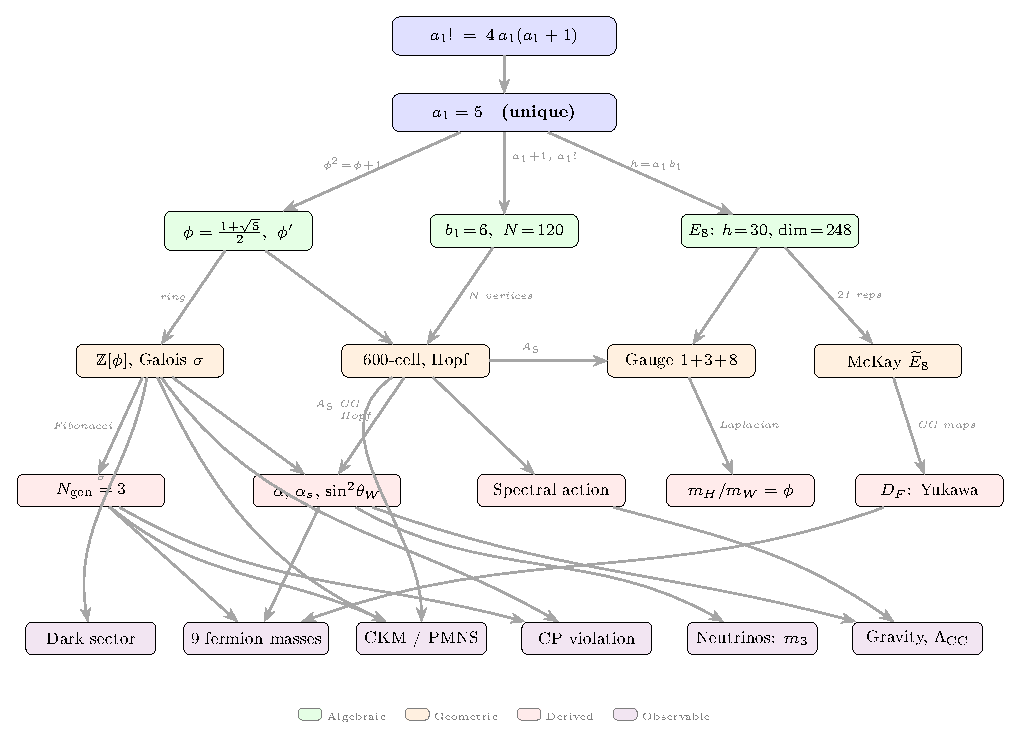
\includegraphics[width=\textwidth]{flow_diagram.pdf}
\caption{Derivation tree from $a_1 = 5$.  Green: algebraic consequences.  Orange: geometric/structural objects.  Red: derived physics.  Violet: observables.  Every arrow represents a deduction with zero free parameters (except $m_e$, the dimensional anchor).}
\label{fig:flow}
\end{figure}

\subsection{Self-Reference and the Golden Ratio}

Equation~\eqref{eq:selfreference} already encodes the structure of a topological quantum field theory.  Its positive root $\phi = (1 + \sqrt{5})/2$ satisfies $\phi = 1 + 1/\phi$: the whole equals one plus its own inverse.  Reinterpreted as a fusion rule for anyonic excitations,
\begin{equation}
\tau \otimes \tau = \mathbf{1} \oplus \tau,
\label{eq:fibonacci_fusion}
\end{equation}
this equation defines the Fibonacci anyon category: two copies of the fundamental excitation combine to produce either the vacuum~($\mathbf{1}$) or a new copy of themselves~($\tau$).  The quantum dimension is $d_\tau = \phi$, and every iterated fusion decomposes via $\phi^n = F_n\,\phi + F_{n-1}$ (Fibonacci numbers), giving the theory a \emph{fractal} self-similar structure at every level.

The fusion matrix
\[
N_\tau = \begin{pmatrix} 0 & 1 \\ 1 & 1 \end{pmatrix}
\]
has eigenvalues $\phi$ and $\phi' = -1/\phi$: the physical sector and the Galois-conjugate (dark) sector are the two eigenvalues of self-observation.

\subsection{Vacuum Selection: the Bootstrap Theorem}
\label{sec:bootstrap}

The Fibonacci fusion rule~\eqref{eq:fibonacci_fusion} selects a \emph{unique} integer.  Each positive integer $a_1 \ge 3$ determines both an algebraic parameter $\phi(a_1) = (1 + \sqrt{a_1})/2$ and an $SU(2)$ Chern--Simons theory at level $k = a_1 - 2$, whose $j = 1$ quantum dimension is
\begin{equation}
d_1(a_1) = \frac{\sin(3\pi/a_1)}{\sin(\pi/a_1)} = 1 + 2\cos\!\Big(\frac{2\pi}{a_1}\Big).
\end{equation}
Demanding that the algebraic parameter equal the quantum dimension of the theory it generates---a \emph{bootstrap} self-consistency condition---gives
\begin{equation}
\label{eq:bootstrap}
\boxed{d_1 = \phi(a_1) \quad\Longleftrightarrow\quad \cos\!\Big(\frac{2\pi}{a_1}\Big) = \frac{\sqrt{a_1} - 1}{4}}
\end{equation}

\begin{theorem}[TQFT Bootstrap Vacuum Selection]
\label{thm:bootstrap}
The only positive integer $a_1$ satisfying~\eqref{eq:bootstrap} is $a_1 = 5$.
\end{theorem}

\begin{proof}
Write $f(a_1) = \cos(2\pi/a_1) - (\sqrt{a_1} - 1)/4$.\\
\emph{Upper bound.}  For $a_1 \ge 26$, $(\sqrt{a_1} - 1)/4 > 1 \ge |\cos(\cdot)|$, so $f < 0$.\\
\emph{Finite check.}  For $a_1 = 1, \dots, 25$, exhaustive evaluation shows $f(a_1) = 0$ only at $a_1 = 5$.\\
\emph{Exactness.}  For $a_1 = 5$: $\cos(2\pi/5)$ is a root of $4x^2 + 2x - 1 = 0$, whose positive root is $(\sqrt{5} - 1)/4$.  Hence $f(5) = 0$ exactly.
\end{proof}

\begin{corollary}[Double embedding]
\label{cor:double}
$d_{1/2}(a_1) = 2\cos(\pi/a_1) = \phi(a_1)$ also holds if and only if $a_1 = 5$.  Thus both the $j = \tfrac12$ and $j = 1$ quantum dimensions equal $\phi$, giving the spectrum $\{d_j\} = \{1, \phi, \phi, 1\}$.
\end{corollary}

\begin{proof}
$2\cos(\pi/a_1) = \phi(a_1)$ iff $\cos(\pi/5) = (1+\sqrt{5})/4$, the positive root of $4x^2 - 2x - 1 = 0$.  The equality $d_{1/2} = d_1$ reduces to $x^2 - x - 1 = 0$ (the golden ratio equation), which requires $a_1 = 5$ uniquely.
\end{proof}

\paragraph{Physical interpretation.}
The parameter $a_1$ simultaneously defines three structures:
\begin{enumerate}
\item[(i)] the number field $\mathbb{Q}(\sqrt{a_1})$ with ring of integers $\mathbb{Z}[\phi]$;
\item[(ii)] a topological quantum field theory via $SU(2)$ Chern--Simons at level $k = a_1 - 2$;
\item[(iii)] the quantum dimension $d_1$ of the $j = 1$ representation.
\end{enumerate}
Self-consistency requires the \emph{number} from~(i) to equal the \emph{quantum dimension} from~(iii).  This is a fixed-point condition $\phi(a_1) = d_1(a_1)$ with a unique solution $a_1 = 5$.  The theory selects itself: the algebraic parameter \emph{is} the quantum dimension.  The Chern--Simons theory and its physical consequences (Fibonacci anyons, Verlinde ring, topological entanglement) are developed in Section~\ref{sec:tqft}.

\subsection{Geometric Characterisation}

The integer $a_1 = 5$ selected by the bootstrap admits a Diophantine characterisation:
\begin{equation}
\boxed{a_1! = 4\,a_1\,(a_1 + 1)}
\label{eq:diophantine}
\end{equation}
\textbf{Unique solution:} $5! = 120 = 4 \times 5 \times 6$.  The left side is the order of the binary icosahedral group $2I$, which permutes the 120 vertices of the 600-cell.  The right side is $4 \times (\text{diameter}) \times (\text{distance classes})$ of the 600-cell Cayley graph.  This is a self-consistency condition between the symmetry group and the geometry it acts on: the group order equals a product of its own graph invariants.  For $a_1 \ge 6$ the factorial outgrows $4a_1^2$, so no further solutions exist.

\subsection{What \texorpdfstring{$a_1 = 5$}{a1 = 5} Determines}
\label{sec:cascade}

Define $b_1 \equiv a_1 + 1 = 6$. The cascade of derived quantities is:

\begin{table}[H]
\centering
\begin{tabular}{llll}
\toprule
\textbf{Quantity} & \textbf{Formula} & \textbf{Value} & \textbf{Physical role} \\
\midrule
$\phi$ & $(1 + \sqrt{a_1})/2$ & $(1+\sqrt{5})/2$ & Golden ratio, scaling factor \\
$\phi'$ & $(1 - \sqrt{a_1})/2$ & $(1-\sqrt{5})/2$ & Galois conjugate \\
$\text{disc}(\mathbb{Z}[\phi])$ & $a_1$ & 5 & Ring discriminant \\
$N$ & $a_1!$ & 120 & 600-cell vertices = $|2I|$ \\
$h(E_8)$ & $a_1 \cdot b_1$ & 30 & $E_8$ Coxeter number \\
$N_{\text{eig}}$ & sol. of $\binom{n}{2} = b_1^2$ & 9 & Distinct eigenvalues \\
$\text{rank}(E_8)$ & $N_{\text{eig}} - 1$ & 8 & $E_8$ rank \\
$\dim(E_8)$ & $(N_{\text{eig}}-1)(h+1)$ & 248 & $E_8$ dimension \\
$\sin^2\theta_W$ & $b_1/(a_1^2+1)$ & $6/26$ & Weinberg angle \\
$\alpha$ & sol. of $2\pi x^2 - 4a_1\phi^4 x + 1 = 0$ & $1/137.036$ & Fine structure constant \\
$\alpha_s$ & $1/z$: $\text{Tr}=8$, $|N|=4$ & $1/(2\phi^3)$ & Strong coupling \\
$N_{\text{gen}}$ & from Fibonacci on $\mathbb{Z}[\phi]$ & 3 & Fermion generations \\
$m_e/m_P$ & $\alpha^{z_P}$, $z_P = 12\phi^2/3$ (spectral weight of $R_3$) & $\alpha^{4\phi^2}$ & Planck-hierarchy pattern \\
\bottomrule
\end{tabular}
\caption{The cascade from $a_1=5$.  Algebraic entries are exact; physical roles retain the provenance labels in the binding audit.}
\label{tab:cascade}
\end{table}

A remarkable secondary Diophantine reinforces the uniqueness:
\begin{equation}
(a_1 - 2)! = a_1 + 1 \qquad \Longrightarrow \qquad 3! = 6 \quad \checkmark
\label{eq:secondary_dioph}
\end{equation}
which also has $a_1 = 5$ as its unique solution (re-derived independently from the Galois norm cubic identity in Section~\ref{sec:norm_sum}). The number 5 is simultaneously the graph diameter, the discriminant of $\mathbb{Z}[\phi]$, and $|2I/2T|$ (cosets of the binary tetrahedral in the binary icosahedral group).

A complete notation table is provided in Supplementary Material~S1.



%==============================================================
\section{The 600-Cell and the Hopf Fibration}
\label{sec:geometry}
%==============================================================

The integer $a_1 = 5$ determines a unique geometry.  The 600-cell $\{3,3,5\}$ is a regular 4-dimensional polytope whose $120 = a_1!$ vertices lie on $S^3$:

\begin{center}
\begin{tabular}{ll}
\toprule
Vertices & $120 = a_1!$ \\
Edges & $720 = 120 \times 12 / 2$ \\
Faces (triangles) & 1200 \\
Cells (tetrahedra) & 600 \\
Symmetry group $H_4$ & Order 14,400 \\
Graph diameter & $5 = a_1$ \\
Vertex degree & $12 = 2\,b_1$ \\
\bottomrule
\end{tabular}
\end{center}

\textbf{Universal optimality.} By the Cohn--Kumar theorem \cite{cohn2007,cohn2022}, the 120 vertices of the 600-cell form the \emph{unique} universally optimal spherical code on $S^3$: they minimize the energy for \emph{every} completely monotonic potential simultaneously. This is not an assumption but a theorem---any attractive pairwise interaction on $S^3$ produces this configuration. The discreteness is forced by energy minimization, just as the hexagonal lattice (2D) and FCC structure (3D) are forced by close-packing. The 600-cell is not chosen; it is the unique answer to ``what is the optimal discrete geometry on $S^3$?''

\subsection{Spectral Structure}

The 600-cell graph is distance-transitive with an association scheme of $N_{\text{eig}} = 9$ classes. Its adjacency matrix has exactly 9 distinct eigenvalues, all in $\mathbb{Z}[\phi]$:

\begin{table}[H]
\centering
\begin{tabular}{cccl}
\toprule
\textbf{Index} & \textbf{Eigenvalue} $\lambda_i$ & \textbf{Multiplicity} & \textbf{Structure} \\
\midrule
0 & $12$ & $1 = 1^2$ & Trivial \\
1 & $6\phi$ & $4 = 2^2$ & $\phi$-sector \\
2 & $4\phi$ & $9 = 3^2$ & $\phi$-sector \\
3 & $3$ & $16 = 4^2$ & Rational \\
4 & $0$ & $25 = 5^2$ & Kernel \\
5 & $-2$ & $36 = 6^2$ & Rational \\
6 & $4 - 4\phi$ & $9 = 3^2$ & $\phi'$-sector \\
7 & $-3$ & $16 = 4^2$ & Rational \\
8 & $6 - 6\phi$ & $4 = 2^2$ & $\phi'$-sector \\
\bottomrule
\end{tabular}
\caption{600-cell adjacency spectrum. All eigenvalues are of the form $a + b\phi$ with $a,b \in \mathbb{Z}$, and all multiplicities are perfect squares $n^2$. The intersection numbers are $a_1 = 5$, $b_1 = 6$.}
\label{tab:spectrum}
\end{table}

\textbf{Key structural facts:} (i) Every multiplicity is a perfect square---the irreducible representation dimensions of $2I$ squared. (ii) The $\phi$-dependent eigenvalues (those with $b \neq 0$) have total dimension $4 + 9 + 9 + 4 = 26$, split symmetrically between $\phi$- and $\phi'$-sectors ($13 + 13$). (iii) The intersection numbers $a_1 = 5$ and $b_1 = 6$ determine the mass formula (Section~\ref{sec:masses}).

\subsection{The \texorpdfstring{$E_8$}{E8} Connection}

The $E_8$ root system is constructed from the 600-cell via the icosian lattice \cite{conway1998icosian,elser1987}. Each vertex $v = (v_0, v_1, v_2, v_3)$ with $v_i = a_i + b_i\phi$ maps to an 8-tuple $(a_0, b_0, \ldots, a_3, b_3) \in \mathbb{R}^8$.  The \emph{Galois conjugation} $\sigma: \phi \to \phi' = (1-\sqrt{5})/2$ is the unique non-trivial automorphism of the number field $\mathbb{Q}(\sqrt{5})$; it sends $\sqrt{5} \to -\sqrt{5}$ while fixing all rational numbers.  Physically, $\sigma$ will play the role of a discrete symmetry that distinguishes the visible and dark sectors (Section~\ref{sec:dark}).  Applying $\sigma$ to the vertex coordinates defines a second copy $T = \phi' \cdot S$. Then:
\begin{equation}
\boxed{E_8 \text{ roots} = S \cup T, \qquad |S| = |T| = 120, \qquad S \cap T = \emptyset, \qquad |S \cup T| = 240}
\end{equation}
The inner product structure matches $E_8$ exactly (240/240 roots verified by Procrustes alignment). The 24 Galois-fixed vertices ($b_i = 0$ for all $i$) form the $D_4$ root system, providing a second derivation of the gauge/fermion split:
\begin{equation}
120 = \underbrace{24}_{\text{Galois-fixed} \;=\; D_4 \;=\; \text{gauge}} \;+\; \underbrace{96}_{\text{Galois-moving} \;=\; \text{fermions}}
\end{equation}

The Coxeter number $h(E_8) = 30 = a_1 \cdot b_1$, the rank $= 8 = N_{\text{eig}} - 1$, and $\dim(E_8) = 248 = 8 \times 31 = (N_{\text{eig}}-1)(h+1)$.



\subsection{The Hopf Fibration}

The 3-sphere $S^3$ carries the Hopf fibration $\pi: S^3 \to S^2$ with fiber $S^1$.  On the 600-cell, the group structure of $2I$ partitions the 12 nearest neighbors of each vertex into $2$ fiber neighbors and $10$ cross-fiber neighbors.  The 720 edges decompose as:
\begin{equation}
720 = \underbrace{120}_{\text{fiber edges}} \;+\; \underbrace{600}_{\text{cross edges}}, \qquad
\text{fiber degree} = 2, \qquad \text{cross degree} = 10
\end{equation}
The 120 fiber edges form 12 disjoint $C_{10}$ cycles (the Hopf fibers), each carrying the $\mathbb{Z}_{10}$ cyclic structure of the fiber.  This decomposition defines two Laplacians $L_{\mathrm{fiber}}$ and $L_{\mathrm{cross}}$ with $L = L_{\mathrm{fiber}} + L_{\mathrm{cross}}$ (where $L = \mathrm{deg}\cdot I - A$ is the graph Laplacian).  These two operators \emph{commute}:
\begin{equation}
[L_{\mathrm{fiber}},\, L_{\mathrm{cross}}] = 0
\label{eq:fiber_cross_commute}
\end{equation}
This is a theorem, not a numerical observation: the 600-cell Cayley graph has adjacency matrix $A = \sum_{s \in S} P_s$ where $S$ is the $12$-element generating set and $P_s$ is left-multiplication by~$s$.  Since $S$ forms a single conjugacy class of~$2I$, the partition $S = S_{\mathrm{fiber}} \sqcup S_{\mathrm{cross}}$ (with $|S_{\mathrm{fiber}}| = 2$, $|S_{\mathrm{cross}}| = 10$) is stable under conjugation by any fiber generator~$g$: both elements of $S_{\mathrm{fiber}}$ lie in the abelian subgroup~$C_{10}$, so $g\,S_{\mathrm{fiber}}\,g^{-1} = S_{\mathrm{fiber}}$ and hence $g\,S_{\mathrm{cross}}\,g^{-1} = S_{\mathrm{cross}}$.  The product identity $\{fc : f \!\in\! S_{\mathrm{fiber}},\, c \!\in\! S_{\mathrm{cross}}\} = \{cf : c \!\in\! S_{\mathrm{cross}},\, f \!\in\! S_{\mathrm{fiber}}\}$ then follows from $fc = (fcf^{-1})f$ with $fcf^{-1} \in S_{\mathrm{cross}}$, yielding $A_{\mathrm{fiber}}\,A_{\mathrm{cross}} = A_{\mathrm{cross}}\,A_{\mathrm{fiber}}$ and hence~\eqref{eq:fiber_cross_commute} (verified numerically across all 27 Hopf fibrations to machine precision).

Commutativity implies the eigenspaces decompose simultaneously: every eigenvector of $L$ is simultaneously an eigenvector of $L_{\mathrm{fiber}}$ and $L_{\mathrm{cross}}$.


%==============================================================
\section{The Wave Operator}
\label{sec:operator}
%==============================================================

The Hopf fibration of Section~\ref{sec:geometry} determines a canonical wave operator on the 600-cell.  We show that this operator is \emph{derived}, not chosen: a variational principle on the fiber-cross decomposition selects it uniquely.

\subsection{The Galois Kernel Theorem}
\label{sec:galois_kernel}

The Hopf fibration induces a spectral decomposition that selects exactly one irrep from each Galois orbit of~$2I$.  Define the \emph{Lorentzian operator} $\Box = b_1 \, A_{\text{fiber}} - A$, where $A_{\text{fiber}}$ is the fiber adjacency.

\begin{theorem}[Galois Kernel Theorem]\label{thm:galois_kernel}
On the 600-cell with any Hopf fibration:
\begin{equation}
\ker(\Box) = \ker(b_1\,A_{\mathrm{fiber}} - A) = \rho_0 \oplus \rho_1 \oplus \rho_8, \qquad
\dim(\ker) = 1 + 4 + 4 = 9 = N_{\mathrm{eig}}
\label{eq:galois_kernel}
\end{equation}
The kernel selects the smallest irrep from each Galois orbit, with $\sum \dim = 1+2+2 = 5 = a_1$.  Among all integers $c$, only $c = b_1 = 6$ gives this nontrivial kernel.
\end{theorem}

\noindent\textit{Proof sketch.}  The kernel condition requires $\lambda_A/b_1$ to match a $C_{10}$ cycle eigenvalue $2\cos(k\pi/a_1)$.  Only $\rho_0$ ($\lambda = 12$), $\rho_1$ ($\lambda = 6\phi$), and $\rho_8$ ($\lambda = 6\phi'$) satisfy this; all other eigenvalue ratios fail to match.  See Supplementary Material~S7.2 for the full proof, including verification across all 27 Hopf fibrations.  \hfill$\square$

\begin{theorem}[Trace--Bootstrap Equivalence]\label{thm:trace_bootstrap}
$\mathrm{Tr}(\Box^{N_{\mathrm{gen}}}) = N^2$ if and only if $a_1 = 5$.
\end{theorem}

\noindent\textit{Proof.}  Since $[A_{\mathrm{fiber}}, A_{\mathrm{cross}}] = 0$, expand $\Box^3 = (a_1 A_{\mathrm{fiber}} - A_{\mathrm{cross}})^3$ by the binomial theorem.  The four mixed traces evaluate by triangle counting:
\begin{itemize}
\item $\mathrm{Tr}(A_{\mathrm{fiber}}^3) = 0$: the fiber graph ($C_{10}$ cycles, girth~$10$) has no triangles.
\item $\mathrm{Tr}(A_{\mathrm{fiber}}^2 A_{\mathrm{cross}}) = 0$: no triangle has two fiber edges (the 1200 triangles split as $T_0 = T_1 = 600$ with $0$ or $1$ fiber edges; $T_2 = T_3 = 0$).
\item $\mathrm{Tr}(A_{\mathrm{fiber}} A_{\mathrm{cross}}^2) = 2T_1 = 1200$: each of the $600$ one-fiber-edge triangles contributes~$2$ (two walk orientations).
\item $\mathrm{Tr}(A_{\mathrm{cross}}^3) = 6T_0 = 3600$: each of the $600$ all-cross triangles contributes~$6$.
\end{itemize}
Hence $\mathrm{Tr}(\Box^3) = 3a_1 \cdot 2T_1 - 6T_0 = 6T_0(a_1 - 1)$, using $T_1 = T_0$.  Setting $\mathrm{Tr}(\Box^3) = N^2$ with $T_0 = a_1 N$ gives $6a_1(a_1-1)N = N^2$, i.e.\ $b_1 a_1(a_1-1) = a_1!$, equivalently $(a_1-2)! = a_1 + 1$.  Among integers $a_1 \ge 2$, the unique solution is $a_1 = 5$ ($3! = 6$). This is exactly the bootstrap equation~\eqref{eq:bootstrap} in the form $(a_1-2)! = b_1$.\hfill$\square$

Moreover, $n = N_{\mathrm{gen}} = 3$ is the \emph{unique} positive integer satisfying $\mathrm{Tr}(\Box^n) = N^2$: for $n \le 2$ the trace is too small ($\mathrm{Tr}(\Box^2) = 7200 < N^2$), while for $n \ge 4$ it is too large ($\mathrm{Tr}(\Box^4) = 756000 \gg N^2$), with subsequent moments growing monotonically.  Thus the wave operator simultaneously selects $a_1 = 5$ (from the identity) and $N_{\mathrm{gen}} = 3$ (as the unique crossing exponent), providing an independent derivation of the generation count from the Lorentzian spectrum.

The identity $\mathrm{Tr}(\Box^{a_1}) = \mathrm{Tr}(\Box^5) = (2a_1)! = |S_{2a_1}|$ is verified by exact arithmetic in~$\mathbb{Z}[\sqrt{5}]$ (Supplementary Material); whether it is independently equivalent to the bootstrap remains open.

\begin{theorem}[Variational Bootstrap]\label{thm:variational_bootstrap}
Consider the one-parameter family $\Box(c) = c\, A_{\mathrm{fiber}} - A$ on the 600-cell vertex graph.  The polynomial
\begin{equation}
\mathrm{Tr}\!\big(\Box(c)^{N_{\mathrm{gen}}}\big) \;=\; 3\,N_f\,(c - 2)
\label{eq:variational_linear}
\end{equation}
is \textbf{linear} in~$c$, and the condition $\mathrm{Tr}(\Box(c)^3) = N^2$ has the \textbf{unique} solution
\begin{equation}
\boxed{c \;=\; \frac{N^2}{3\,N_f} + 2 \;=\; \frac{N}{h} + 2 \;=\; (a_1-1) + 2 \;=\; b_1}
\label{eq:variational_c}
\end{equation}
where $h=a_1b_1=30$ is the Coxeter number of $E_8$ and the additive constant $2$ is the fiber degree.  The quotient $N/h=a_1-1=4$ is exact arithmetic; it is not a spacetime dimension.  The operator $\Box=b_1A_{\mathrm{fiber}}-A$ is thereby fixed by the stated bootstrap condition.
\end{theorem}

\begin{proof}
Expand $\mathrm{Tr}((cF - A)^3) = \alpha_3 c^3 + \alpha_2 c^2 + \alpha_1 c + \alpha_0$ where $F = A_{\mathrm{fiber}}$.  Using the cyclic property of the trace and the classification of the $1200$ triangles into $T_0 = T_1 = 600$ (with $0$ or $1$ fiber edge) and $T_2 = T_3 = 0$:
\begin{itemize}
\item $\alpha_3 = \mathrm{Tr}(F^3) = 0$: the Hopf fibers ($C_{10}$ cycles, girth $10$) admit no triangles.
\item $\alpha_2 = -3\,\mathrm{Tr}(F^2 A) = 0$: a length-$3$ walk using two fiber edges stays in a single fiber, and vertices at distance~$2$ in $C_{10}$ are not adjacent.
\item $\alpha_1 = 3\,\mathrm{Tr}(F A^2) = 3\,N_f$: each directed fiber edge contributes its $5$ containing triangles.
\item $\alpha_0 = -\mathrm{Tr}(A^3) = -6\,N_f$: counts all $N_f$ triangles with multiplicity~$6$.
\end{itemize}
All four values are computed in exact integer arithmetic (\texttt{int64}).  Hence $P(c)=3N_f(c-2)$ and $P(c)=N^2$ gives $c=N^2/(3N_f)+2$.  Substituting $N_f=Nh/3$ yields $c=N/h+2=(a_1-1)+2=b_1$.  These are combinatorial equalities; no spacetime dimension is used.
\end{proof}

\noindent\textit{Remark.}  The vanishing of $\alpha_3$ and $\alpha_2$ is not numerical coincidence but a consequence of the Hopf fiber geometry: the C$_{10}$ cycles have girth~$10 > 3$, which eliminates all-fiber triangles and two-fiber-edge triangles simultaneously.  This reduces a potentially cubic variational problem to a \emph{linear equation with a unique solution}.  The three levels of self-reference are: $x^2 = x + 1$ defines the number field; $a_1! = 4a_1(a_1\!+\!1)$ selects the polytope; $\mathrm{Tr}(\Box(c)^3) = N^2$ determines the operator.



%==============================================================
\section{The Vertex Spectrum: Speed of Light and Mass}
\label{sec:vertex_spectrum}
%==============================================================

The wave operator $\Box$ of Section~\ref{sec:operator}, applied to the 120 vertices of the 600-cell, determines the propagation speed, the discrete mass spectrum, and the mass hierarchy through the McKay correspondence.

\paragraph{The speed of light from spectral gaps.}
The spectral gaps are:
\begin{equation}
\lambda_1(L_{\mathrm{fiber}}) = 2 - \phi, \qquad
\lambda_1(L_{\mathrm{cross}}) = 10 - 5\phi = a_1\,(2 - \phi), \qquad
\frac{\lambda_1(L_{\mathrm{cross}})}{\lambda_1(L_{\mathrm{fiber}})} = a_1 = 5
\label{eq:spectral_gap_ratio}
\end{equation}
The operator historically denoted $\Box$ has the algebraic form $\Box=L_{\mathrm{cross}}-a_1L_{\mathrm{fiber}}$.  Under the additional normalization that reads the two terms as a lattice update, its dimensionless coefficient is
\begin{equation}
\boxed{c_{\mathrm{lat}}^2 = a_1 = 5}
\label{eq:c_squared}
\end{equation}
in lattice units, i.e.\ a dimensionless propagation coefficient $c_{\mathrm{lat}}=\sqrt{a_1}=\sqrt{5}=2\phi-1$.  This finite coefficient is derived.  Identifying one lattice edge and one update tick with physical length and time, and identifying the corresponding mode with light, are additional dictionaries; therefore neither the SI speed of light nor its claimed unification with the fine-structure constant is derived here.  The reuse of the same Hopf-fiber arithmetic is an exact structural relation, while its physical causal interpretation remains open.

\paragraph{Trace moment identities.}
Although the eigenvalues of $\Box$ are individually irrational ($\in \mathbb{Z}[\sqrt{5}]$), all trace moments $\mathrm{Tr}(\Box^n)$ are \emph{exact integers} for $n = 1, \ldots, 12$ (verified by exact arithmetic in~$\mathbb{Z}[\sqrt{5}]$; all $\sqrt{5}$ contributions cancel term by term).  The key identities, also fibration-independent, are:
\begin{equation}
\frac{\mathrm{Tr}(\Box^2)}{N} = 60 = \mathrm{deg}\cdot a_1, \qquad
\mathrm{Tr}(\Box^3) = N^2, \qquad
\mathrm{Tr}(\Box^5) = (2a_1)!
\label{eq:box_traces}
\end{equation}


\paragraph{Discrete dispersion relation and mass spectrum.}
Since $[L_{\mathrm{fiber}}, L_{\mathrm{cross}}] = 0$, the operators share a simultaneous eigenbasis. Each mode~$i$ has joint eigenvalues $(\lambda_f^{(i)}, \lambda_c^{(i)})$ with $\lambda_f^{(i)} \in \{0,\, 2\!-\!\phi,\, 3\!-\!\phi,\, 1\!+\!\phi,\, 2\!+\!\phi,\, 4\}$ (the $C_{10}$ cycle spectrum) and a discrete ``mass'' $\mu^{(i)} = \lambda_c^{(i)} - a_1\,\lambda_f^{(i)}$.  The effective speed $c_{\mathrm{eff}}^2 \equiv \langle\lambda_c\rangle/\langle\lambda_f\rangle$ equals~$a_1$ \emph{exactly at every angular momentum level} $l = 0, 1, \ldots, 5$ and at each Galois-conjugate level, not only at the spectral gap.  This follows from $\mathrm{Tr}(\Box|_{E_\lambda}) = 0$ restricted to each Laplacian eigenspace~$E_\lambda$.

The 120 modes decompose into 9 massless (the $\ker\Box$ light cone) and 111 massive modes with 12 distinct mass values, all algebraic in~$\mathbb{Z}[\phi]$.  The two smallest nonzero masses are:
\begin{equation}
|\mu_1| = \frac{b_1}{\phi} - 2 = 6\phi - 8, \qquad
|\mu_2| = a_1 - \sqrt{a_1} = 5 - \sqrt{5}, \qquad
\frac{|\mu_2|}{|\mu_1|} = \phi
\label{eq:mass_ratio_phi}
\end{equation}
The golden ratio appears as the \emph{first mass ratio} of the discrete wave operator.  This is exact: rationalizing $(5\!-\!\sqrt{5})/(6\phi\!-\!8) = (5\!-\!\sqrt{5})/({-}5\!+\!3\sqrt{5})$ yields $20\phi/20 = \phi$.  The full mass spectrum $\{|\mu|\} = \{0,\, 6\phi\!-\!8,\, 5\!-\!\sqrt{5},\, 6/\phi,\, 10\!-\!2\sqrt{5},\, 6\phi\!-\!3,\, 5\!+\!\sqrt{5},\, 6\phi,\, 10,\, 6\phi\!+\!2,\, 12,\, 10\!+\!2\sqrt{5}\}$ is fully determined by~$a_1$.

\paragraph{McKay correspondence and the mass spectrum.}
The McKay correspondence maps the $9$ irreps of~$2I$ to the nodes of the extended $E_8$ Dynkin diagram.  The kernel of~$\Box$ selects $\rho_0$, $\rho_1$, $\rho_8$---exactly the three \emph{extremal} nodes (the tips of the diagram).  The mean mass $\langle|\mu|\rangle$ per irrep increases monotonically with the graph distance from these extremal nodes:
\begin{center}
\begin{tabular}{clc}
\toprule
Distance & Irreps & Mean $|\mu|$ \\
\midrule
0 & $\rho_0,\, \rho_1,\, \rho_8$ & $0$ (massless) \\
1 & $\rho_2,\, \rho_7$ & $5.20$ \\
2 & $\rho_3,\, \rho_5$ & $7.26$ \\
3 & $\rho_4,\, \rho_6$ & $8.71$ \\
\bottomrule
\end{tabular}
\end{center}
(Pearson correlation $r = 0.93$.)  The wave operator thus encodes the $E_8$ singularity structure: massless modes live at the boundary of the Dynkin diagram, and mass grows radially inward.  Since the 600-cell is the \emph{link} of the $E_8$ singularity $\mathbb{C}^2/2I$, this realizes a self-referential loop: the singularity defines the link, the link carries the wave operator~$\Box$, and $\Box$ reconstructs the singularity's Dynkin diagram through its mass spectrum.



%==============================================================
\section{Gauge Group from the 600-Cell}
\label{sec:gauge}
%==============================================================

The 24 non-fermionic vertices (Types A and B: cross-polytope + tesseract) form the $D_4$ root system, which is the 24-cell. The 96 remaining vertices decompose as
\begin{equation}
96 = 16 \times 3 \times 2 = \text{(fermions per generation)} \times \text{(generations)} \times \text{(chiralities)}
\end{equation}

\textbf{Representation-theoretic derivation.}  The 12 nearest neighbors of any vertex form an \emph{icosahedron} (the vertex figure of the 600-cell), whose rotation group is $A_5\cong 2I/\mathbb{Z}_2$.  The permutation representation of $A_5$ on the 12 icosahedron vertices has character $\chi(e)=12$, $\chi(\text{double transposition})=0$, $\chi(\text{3-cycle})=0$, $\chi(\text{5-cycle})=2$, which decomposes as
\begin{equation}
12 \;=\; \mathbf{1} \;\oplus\; \mathbf{3} \;\oplus\; \mathbf{3'} \;\oplus\; \mathbf{5}
\label{eq:A5decomp}
\end{equation}
where $\mathbf{3}$ and $\mathbf{3'}$ are the two inequivalent 3-dimensional irreps of $A_5$, distinguished by the Galois automorphism $\phi\leftrightarrow\phi'$ (their characters on 5-cycles are $\phi$ and $\phi'$ respectively).

Now embed $A_5\subset SO(3)\subset SU(3)$ via the $\mathbf{3}$-irrep.  The adjoint of $SU(3)$ restricts to $A_5$ as
\begin{equation}
\mathrm{ad}(SU(3))\big|_{A_5} \;=\; \mathbf{3}\otimes\mathbf{3} - \mathbf{1} \;=\; \mathbf{3} \oplus \mathbf{5}
\qquad (\dim = 8)
\end{equation}
since $\mathbf{3}\otimes\mathbf{3} = \mathbf{1}\oplus\mathbf{3}\oplus\mathbf{5}$ (verified via character inner products).  The permutation decomposition~\eqref{eq:A5decomp} therefore becomes
\begin{equation}
\boxed{12 \;=\; \underbrace{\mathbf{1}}_{U(1)} \;+\; \underbrace{\mathbf{3'}}_{=\,\mathrm{ad}(SU(2))} \;+\; \underbrace{\mathbf{3}\oplus\mathbf{5}}_{=\,\mathrm{ad}(SU(3))} \;=\; 1 + 3 + 8}
\label{eq:gauge138}
\end{equation}
This is the \emph{only} valid grouping.  To see why, enumerate all partitions of $\{\mathbf{1},\mathbf{3},\mathbf{3'},\mathbf{5}\}$ into sub-sums and check which produce adjoint dimensions of simple Lie groups ($\mathrm{ad}(SU(n)) = n^2 - 1$, so the allowed adjoint dimensions $\leq 12$ are $3, 8$):
\begin{center}\small
\begin{tabular}{lcc}
\toprule
\textbf{Grouping} & \textbf{Dimensions} & \textbf{Adjoint?} \\
\midrule
$\{\mathbf{1}\} + \{\mathbf{3'}\} + \{\mathbf{3},\mathbf{5}\}$ & $1 + 3 + 8$ & \textbf{Yes}: $U(1) + SU(2) + SU(3)$ \\
$\{\mathbf{1}\} + \{\mathbf{3}\} + \{\mathbf{3'},\mathbf{5}\}$ & $1 + 3 + 8$ & \textbf{Yes}: Galois conjugate of above \\
$\{\mathbf{1}\} + \{\mathbf{5}\} + \{\mathbf{3},\mathbf{3'}\}$ & $1 + 5 + 6$ & No: $5 \neq n^2\!-\!1$; $6 \neq n^2\!-\!1$ \\
$\{\mathbf{1}\} + \{\mathbf{3},\mathbf{3'},\mathbf{5}\}$ & $1 + 11$ & No: $11 \neq n^2\!-\!1$ \\
$\{\mathbf{1},\mathbf{3}\} + \{\mathbf{3'},\mathbf{5}\}$ & $4 + 8$ & No: $4 \neq n^2\!-\!1$ \\
$\{\mathbf{1},\mathbf{3'}\} + \{\mathbf{3},\mathbf{5}\}$ & $4 + 8$ & No: $4 \neq n^2\!-\!1$ \\
$\{\mathbf{1},\mathbf{5}\} + \{\mathbf{3},\mathbf{3'}\}$ & $6 + 6$ & No: $6 \neq n^2\!-\!1$ \\
$\{\mathbf{1},\mathbf{3},\mathbf{3'}\} + \{\mathbf{5}\}$ & $7 + 5$ & No: neither is $n^2\!-\!1$ \\
\bottomrule
\end{tabular}
\end{center}
Only the first two rows produce valid adjoint decompositions, and they are related by the Galois automorphism $\phi\leftrightarrow\phi'$ (which swaps $\mathbf{3}\leftrightarrow\mathbf{3'}$).  The physical choice $\phi > 0$ breaks this discrete symmetry, selecting a unique assignment.

The connection to the McKay correspondence is immediate: the first three nodes of $\widetilde{E}_8$ carry marks $1, 2, 3$ (irrep dimensions of $2I$), and the corresponding $SU(d)$ adjoints have dimensions $1, 2^2-1, 3^2-1 = 1, 3, 8$.  The identity $1 + 3 + 8 = 12 = \text{vertex degree}$ is thus not a coincidence but a consequence of the fact that the permutation representation on the vertex figure decomposes into exactly the adjoint representations selected by the McKay marks.  It is essential to distinguish this \emph{gauge dimension} decomposition $12 = 1 + 3 + 8$ from the \emph{$A_5$ irrep} decomposition $12 = \mathbf{1} \oplus \mathbf{3} \oplus \mathbf{3'} \oplus \mathbf{5}$ (Eq.~\ref{eq:adjoint_constraint}): the bridge is that $\mathrm{ad}(\mathfrak{su}(3))|_{A_5} = \mathbf{3'} \oplus \mathbf{5}$ has dimension $3 + 5 = 8$ (proven in Theorem~\ref{thm:gauge_id}).  The $E_8$ Dynkin diagram branches at the $D_4$ node into three legs with dimensions $\text{Leg A} = 11 = a_1 + b_1$, $\text{Leg B} = 6 = b_1$, and $\text{Leg C} = 9 = N_{\text{eig}}$, with triality broken by the Kac labels $\{3, 4, 5\}$.

\textbf{Computational verification (edge splitting).}  Each fermionic vertex (type~C, 96 total) has 12 neighbors decomposing by vertex type as $1\text{A} + 2\text{B} + 9\text{C}$, confirmed by direct geometry. The SM assignment follows: $U(1)$: 1~AC edge (perfect matching, topological confinement with gap $= 2$); $SU(2)$: 2~BC edges (charged weak) $+$ 1~CC$^*$ edge (neutral current criterion: shared A neighbor, no shared B); $SU(3)$: 8 regular CC edges (color sector, 288 pure plaquettes reproducing QCD self-interaction).  Thus
\begin{equation}
12 = \underbrace{1}_{U(1)} + \underbrace{2 + 1}_{SU(2)} + \underbrace{8}_{SU(3)} = \dim(\text{SM gauge group})
\end{equation}
verified for all 96 fermion vertices.

The 96 fermionic vertices admit a natural $48+48$ split under the Galois involution $\sigma\!: \phi \to \phi'$, with the 24 gauge vertices being Galois-fixed (their coordinates lie in $\mathbb{Q}$).  This provides a candidate chirality grading algebraically derived from the framework.  We summarize below what is established and what remains open.

\label{sec:anomaly}
\textbf{What is derived.}  (i)~The $48+48$ Galois split exists and is \emph{exact}: each fermionic vertex $v$ has a unique Galois partner $\sigma(v) \neq v$, giving $96/2 = 48$ pairs.  (ii)~The counting $48 = 16 \times 3$ matches the SM content: 16 Weyl fermions per generation times 3 generations.  (iii)~All six anomaly cancellation conditions---$\text{Tr}(Y^3) = 0$, $\text{Tr}(Y) = 0$, $[SU(3)]^2 U(1) = 0$, $[SU(2)]^2 U(1) = 0$, $[SU(3)]^3 = 0$, and Witten's global $SU(2)$ anomaly (4 doublets, even)---are satisfied for the standard hypercharge assignments with 16 left-handed Weyl fermions per generation (verified by exact arithmetic).  The hypercharge values are \emph{uniquely} determined by anomaly cancellation plus charge quantization ($Q = T_3 + Y$), with only one free parameter (overall scale $y_1 = 1/6$).  The 16th fermion---the right-handed neutrino $\nu_R$ as a gauge singlet $(1,1,0)$---is required for anomaly cancellation and enables the seesaw mechanism.

\textbf{Why chirality is hard.}  The 600-cell lives on $S^3$, which is odd-dimensional.  Two no-go results apply: (i)~The simplicial Dirac operator $D = d + d^*$ has index zero on $S^3$ (the Euler characteristic vanishes: $\chi(S^3) = 0$).  No choice of combinatorial Dirac operator can produce a nonzero index on a triangulated $S^3$.  (ii)~In the continuum, the chirality operator $\gamma_5 = \gamma^0 \gamma^1 \gamma^2 \gamma^3$ requires four spacetime dimensions.  On the 3-sphere, there is no intrinsic $\gamma_5$; the Atiyah--Singer index theorem gives $\text{ind}(\cancel{D}) = 0$ for any Dirac operator on $S^3$.  These are \emph{topological} obstructions, not limitations of our framework.

\textbf{Possible resolution.}  The Hopf fibration $S^3 \to S^2$ with $S^1$ fibers provides a natural lift from 3 to 4 dimensions: the total space $S^3$ is the principal $U(1)$ bundle over $S^2$, and the extra $S^1$ direction could serve as the ``time-like'' dimension needed for $\gamma_5$.  The Hopf quadrupole $T_3 = a^2 + b^2 - c^2 - d^2$ on $S^3$ produces six distinct values $\pm\phi/2, \pm 1/2, \pm 1/(2\phi)$ on the 96 fermionic vertices, with $48$ positive and $48$ negative---the correct counting for chirality.

\textbf{Status.}  Three ingredients for chirality on the \emph{manifold} are in place: (i)~the Galois grading provides an exact $48 + 48$ split with the correct fermion count $48 = 16 \times N_{\text{gen}}$; (ii)~anomaly cancellation is verified for all six conditions with the standard hypercharge assignments, and the 16th fermion $\nu_R$ is uniquely required; (iii)~the spectral structure (the Hopf quadrupole $T_3$, with 16 vertices per level and 3 levels per sign) reproduces the generation structure $48 = 3 \times 16$.

A fourth ingredient now comes from the \emph{internal} space.  The McKay graph of $2I$ is a tree (9~nodes, 8~edges), hence bipartite.  The unique bipartition assigns chirality $\gamma_F = +1$ (WHITE) to the five integer-spin irreps $\{\rho_1(1),\, \rho_4(3),\, \rho_5(3),\, \rho_6(4),\, \rho_8(5)\}$ with total dimension~16, and $\gamma_F = -1$ (BLACK) to the four half-integer-spin irreps $\{\rho_2(2),\, \rho_3(2),\, \rho_7(4),\, \rho_9(6)\}$ with total dimension~14.  Crucially:
\begin{equation}
\dim(\text{WHITE}) = 16 = (a_1 - 1)^2 = \text{fermions per SM generation}.
\label{eq:white_dim}
\end{equation}
The operator $\gamma_F$ satisfies $\gamma_F^2 = 1$ and $\{\gamma_F, D_F\} = 0$ exactly (a consequence of the tree/bipartite structure: every McKay edge connects WHITE to BLACK).  This identification $\gamma_F = (-1)^{2j}$, where $j$ is the $SU(2)$ spin of the $2I$~irrep, holds for all 9~irreps.  The representation ring $\text{Rep}(2I)$ respects the $\mathbb{Z}/2$~grading: WHITE$\,\otimes\,$WHITE$\,=\,$WHITE, BLACK$\,\otimes\,$BLACK$\,=\,$WHITE, WHITE$\,\otimes\,$BLACK$\,=\,$BLACK (verified for all $9 \times 9 = 81$ tensor products using $A_5$ decomposition).

Taking $T_3(\text{WHITE}) = -\tfrac{1}{2}$ and $T_3(\text{BLACK}) = +\tfrac{1}{2}$ reproduces the SM left-handed weak isospin $T_{3,L}$ for 8 out of 9 fermions; the single failure ($s$~quark) is structural, arising from the $\mu$-$s$ degeneracy at the $w = 0$ McKay edge.  The $SU(2)$ Casimir sum $\sum C_2 = 26 = a_1^2 + 1$ (Eq.~\ref{eq:casimir_sum}) connects $\gamma_F$ to the Weinberg angle.

This internal chirality $\gamma_F$, combined with the product structure, yields the Standard Model chiral gauge coupling.

\begin{theorem}[Chiral gauge coupling]\label{thm:chiral_gauge}
In the product spectral triple $(\mathcal{A},\, \mathcal{H}_M \otimes \mathcal{H}_F,\, D,\, \gamma)$, the Standard Model chirality pattern---$SU(2)$ chiral, $SU(3)$ and $U(1)$ vector-like---is a consequence of the McKay graph structure.
\end{theorem}

\noindent\textit{Proof.}  The gauge group factors correspond to McKay irreps near the trivial node (Theorem~\ref{thm:gauge_id}): $U(1) \leftrightarrow \rho_1$ (dim~1, spin~$0$, WHITE), $SU(2) \leftrightarrow \rho_2$ (dim~2, spin~$\tfrac{1}{2}$, BLACK), $SU(3) \leftrightarrow \rho_4$ (dim~3, spin~$1$, WHITE).  For each irrep~$\sigma$, the tensor product operator $T_\sigma: \mathcal{H}_F \to \mathcal{H}_F$ maps $V_{\rho_k} \to V_{\rho_k \otimes \sigma}$.  Since $\gamma_F$ respects the $\mathbb{Z}/2$ tensor-product grading (verified for all $81$ products):
\begin{itemize}
\item $\gamma_F(\sigma) = +1$ (WHITE): every constituent of $\rho_k \otimes \sigma$ has $\gamma_F = \gamma_F(\rho_k)$, so $[T_\sigma,\, \gamma_F] = 0$ \textup{(vector-like coupling)}.
\item $\gamma_F(\sigma) = -1$ (BLACK): every constituent of $\rho_k \otimes \sigma$ has $\gamma_F = -\gamma_F(\rho_k)$, so $\{T_\sigma,\, \gamma_F\} = 0$ \textup{(chiral coupling)}.
\end{itemize}
The McKay adjacency $D_F$ encodes $T_{\rho_2}$ (the standard representation, spin~$\tfrac{1}{2}$, BLACK): $\{D_F,\, \gamma_F\} = 0$ gives chiral $SU(2)$ coupling.  The $SU(3)$ direction $T_{\rho_4} \sim D_F^2$ and the $U(1)$ direction $T_{\rho_1} = \mathrm{Id}$ both commute with $\gamma_F$, giving vector-like coupling.  Robustness: both dimension-2 irreps ($\rho_2,\, \rho_3$) are BLACK and both dimension-3 irreps ($\rho_4,\, \rho_5$) are WHITE, so the Galois choice $\rho_2 \leftrightarrow \rho_3$, $\rho_4 \leftrightarrow \rho_5$ does not affect the result.  \hfill$\square$

\begin{corollary}\label{cor:left_handed}
In the physical Hilbert space $\mathcal{H}_+ = \{\psi : \gamma\psi = \psi\}$, where $\gamma = \gamma_{\mathrm{form}} \otimes \gamma_F$:
\[
\mathcal{H}_+ = \underbrace{(\mathcal{H}_{\mathrm{even}} \otimes \mathcal{H}_W)}_{\textup{right-handed, $SU(2)$ singlet}} \;\oplus\; \underbrace{(\mathcal{H}_{\mathrm{odd}} \otimes \mathcal{H}_B)}_{\textup{left-handed, $SU(2)$ doublet}}.
\]
Left-handed fermions occupy the BLACK sector ($SU(2)$ doublets) and right-handed fermions the WHITE sector ($SU(2)$ singlets), with $\dim(\mathcal{H}_W) = 16$ fermions per generation.
\end{corollary}

\noindent\textit{Remark.}  The obstacle to chirality on $S^3$ alone is topological ($\mathrm{ind}(D) = 0$).  The theorem shows that the chiral mechanism resides entirely in the \emph{finite} space $F$---specifically in the bipartite structure of the McKay graph---and is therefore independent of the manifold dimension.  The identification $\gamma_{\mathrm{form}} = (-1)^p$ is a theorem about the simplicial Dirac operator $d + d^*$, not an assumption about the spinor $\gamma_5$; the continuum limit (whether $\gamma_{\mathrm{form}}$ reduces to $\gamma_5$ in 4D) remains open (Section~\ref{sec:predictions}).

\noindent\textit{Remark (Lorentzian signature).}  The McKay graph structure permits Lorentzian signature through the KO-dimension mechanism.  On the edge space (dim~$120 = |2I|$), the charge conjugation $J$ satisfies $J^2 = \nu(\rho_i)\,\nu(\rho_j)$ on each edge $(\rho_i, \rho_j)$, where $\nu$ is the Frobenius--Schur indicator.  Since all edges connect nodes of opposite dimension parity (bipartite graph), $J^2$ splits into a dominant sector ($J^2 = -1$, six edges, dim~88) and a subdominant sector ($J^2 = +1$, two edges, dim~32).  Both sectors yield $\varepsilon' = +1$ (from graph symmetry) and $\varepsilon'' = -1$ (from chirality flip under $J$), giving KO-dimension~2 or~6 respectively.  In either case, the Poincar\'e duality condition $\mathrm{KO}(M \times F) \equiv 0\pmod{8}$ forces the spacetime manifold $M$ to have Lorentzian signature $(1,3)$, making the result robust under sector selection.  This parallels the algebra choice $\mathcal{A}_F = \mathbb{C} \oplus \mathbb{H} \oplus M_3(\mathbb{C})$ in standard NCG, where the signature also follows from KO-dimension matching rather than being postulated independently.

\subsection{From Discrete Symmetry to Continuous Gauge Group}
\label{sec:discrete_continuous}

The decomposition~\eqref{eq:gauge138} shows that the $A_5$-module structure of the vertex figure \emph{selects} the Standard Model gauge group from the classification of compact Lie groups.  We now prove this rigorously, addressing the natural objection that a finite group cannot generate a continuous gauge symmetry.

\begin{theorem}[Gauge group identification]\label{thm:gauge_id}
Let $G$ be a compact Lie group with $\dim(G) = 12$, and let $A_5 \subset G$ be a subgroup such that
\begin{equation}
\mathrm{ad}(G)\big|_{A_5} \;=\; \mathbf{1} \oplus \mathbf{3} \oplus \mathbf{3'} \oplus \mathbf{5}
\label{eq:adjoint_constraint}
\end{equation}
as $A_5$-modules.  Then $G \cong U(1) \times SU(2) \times SU(3)$.
\end{theorem}

\noindent\textit{Proof.}  The trivial summand $\mathbf{1}$ in~\eqref{eq:adjoint_constraint} corresponds to an abelian factor: $\mathfrak{g} = \mathfrak{u}(1) \oplus \mathfrak{h}$ where $\mathfrak{h}$ is semisimple with $\dim(\mathfrak{h}) = 11$ and $\mathrm{ad}(\mathfrak{h})|_{A_5} = \mathbf{3} \oplus \mathbf{3'} \oplus \mathbf{5}$.  Write $\mathfrak{h} = \mathfrak{h}_1 \oplus \cdots \oplus \mathfrak{h}_k$ as a direct sum of simple compact Lie algebras.  The dimensions of the simple compact Lie algebras with $\dim \leq 11$ are:
\begin{equation}
\mathfrak{su}(2) : 3, \qquad \mathfrak{su}(3) : 8, \qquad \mathfrak{sp}(2) : 10
\end{equation}
(and $\mathfrak{g}_2 = 14$, $\mathfrak{su}(4) = 15$, etc.).  The \emph{only} partition of $11$ into such dimensions is $11 = 3 + 8$, giving $\mathfrak{h} = \mathfrak{su}(2) \oplus \mathfrak{su}(3)$ and hence $G = U(1) \times SU(2) \times SU(3)$.  (The partition $3 + 3 + 5$ fails because no simple Lie algebra has dimension~$5$; $10 + 1$ fails because $\mathfrak{sp}(2)$ is simple, not $\mathfrak{sp}(2) \oplus \mathfrak{u}(1)$ with dim~$11$.)

For compatibility with~\eqref{eq:adjoint_constraint}, note that $A_5 \subset SO(3) = SU(2)/\mathbb{Z}_2$ via the icosahedral rotation group, giving $\mathrm{ad}(\mathfrak{su}(2))|_{A_5} = \mathbf{3}$ (or $\mathbf{3'}$).  Meanwhile, the tensor product $\mathbf{3} \otimes \mathbf{3} = \mathbf{1} \oplus \mathbf{3} \oplus \mathbf{5}$ (verified by character inner products) gives $\mathrm{ad}(\mathfrak{su}(3))|_{A_5} = \mathbf{3} \otimes \mathbf{3}^* - \mathbf{1} = \mathbf{3} \oplus \mathbf{5}$ (or $\mathbf{3'} \oplus \mathbf{5}$), using the Frobenius--Schur indicator $\nu(\mathbf{3}) = +1$ (real/orthogonal type, so $\mathbf{3}^* \cong \mathbf{3}$).  The two valid assignments are exchanged by the Galois automorphism $\sigma: \sqrt{5} \to -\sqrt{5}$, and $\phi > 0$ selects a unique one. \hfill$\square$

The bridge from discrete to continuous symmetry operates through three complementary mechanisms: (1)~the representation-theoretic decomposition~\eqref{eq:A5decomp} \emph{identifies} the gauge group uniquely (Theorem~\ref{thm:gauge_id}); (2)~Burnside's theorem shows the discrete symmetries \emph{algebraically span} the full gauge Lie algebra (see Supplementary Material~S2); (3)~the spectral action (Section~\ref{sec:spectral_action}) provides the Yang--Mills \emph{dynamics} with continuous gauge invariance.  The hypothesis $\dim(G) = 12$ is not external input: the vertex degree $d = 2(a_1+1) = 12$ determines it.

\noindent\textit{Remark} (Distler--Garibaldi).  The impossibility theorem of~\cite{distler2010} does \emph{not} apply here: the gauge group is identified via the $A_5$ decomposition, and fermions arise from $2I$ irreps---not from $E_8$ representations.  The $E_8$ structure enters exclusively through the McKay correspondence (see Supplementary Material~S2 for details).


\subsection{Edge Gauge Spectrum: Second Derivation}
\label{sec:edge_gauge}

The vertex-figure argument of Section~\ref{sec:gauge} identifies the gauge group from the local geometry around each vertex.  We now give an independent, \emph{global} derivation from the spectrum of the wave operator $\Box$ lifted to the edge space.

\textbf{The line-graph operator.}  Let $L(G)$ be the line graph of the 600-cell: its 720 nodes are the edges of the original graph, connected when they share a vertex.  The Hopf fibration classifies these 720 edges as 120~\emph{fiber edges} (both endpoints in the same Hopf fiber) and 600~\emph{cross edges}.  In $L(G)$, the fiber adjacency $A_{\text{fiber}}$ connects consecutive fiber edges within each $C_{10}$ cycle.  Define
\begin{equation}
\Box_1 \;=\; L_{\text{cross}} - a_1\, L_{\text{fiber}}
\label{eq:box1_def}
\end{equation}
on $L(G)$, in exact analogy with $\Box_0 = L_{\text{cross}} - a_1\, L_{\text{fiber}}$ on the vertex graph.  The matrix $\Box_1$ is $720 \times 720$ with \emph{integer} entries.

\begin{theorem}[Edge gauge spectrum]\label{thm:edge_gauge}
The kernel of $\Box_1$ has dimension $13 = (a_1^2 + 1)/2$ and decomposes under $2I$ as
\begin{equation}
\ker(\Box_1) \;=\; \rho_0 \;\oplus\; 2\,\rho_5
\label{eq:ker_box1}
\end{equation}
where $\rho_0$ is the trivial representation (dim~1) and $\rho_5$ is the 6-dimensional irrep corresponding to the branching node of the affine $E_8$ Dynkin diagram.
\end{theorem}

\noindent\textit{Proof.}\enspace The matrix $\Box_1$ has integer entries (verified), so $\ker(\Box_1) = 720 - \mathrm{rank}(\Box_1) = 720 - 707 = 13$ is exact.  For the irrep decomposition, the character is computed on each of the 9 conjugacy classes of $2I$: $\chi_{\ker}(1) = 13$, $\chi_{\ker}(-1) = -11$.  Applying the decomposition formula $n_\rho = \tfrac{1}{|2I|}\sum_g \overline{\chi_\rho(g)}\,\chi_{\ker}(g)$ yields $n_{\rho_0} = 1$ and $n_{\rho_5} = 2$, with all other multiplicities zero.  The dimension check $1 + 2 \times 6 = 13$ confirms the decomposition.  \hfill$\square$

The 12~gauge modes (the $2\rho_5$ subspace) have a striking geometric character:

\begin{proposition}[Fiber localisation and Hodge eigenvalues]\label{prop:fiber_local}
The 12-dimensional gauge subspace $2\rho_5 \subset \ker(\Box_1)$ satisfies:
\begin{itemize}
\item[\textup{(i)}] \textbf{Fiber localisation:} the 12~modes have support exclusively on the 120 fiber edges (cross-edge weight $< 10^{-29}$);
\item[\textup{(ii)}] \textbf{Coexact eigenvalue:} $C\big|_{2\rho_5} = a_1\, \mathbf{I}_{12}$, where $C = d_1^\top d_1$ is the coexact Hodge Laplacian;
\item[\textup{(iii)}] \textbf{Exact eigenvalue:} $B\big|_{2\rho_5} = \tfrac{16}{a_1}\, \mathbf{I}_{12}$, where $B = d_0\, d_0^\top$ is the exact Hodge Laplacian;
\item[\textup{(iv)}] \textbf{Trace identity:} $\operatorname{Tr}(\Box_1^2)\big/\operatorname{Tr}(\Box_0^2) = 9\,a_1 = 45$.
\end{itemize}
\end{proposition}

\noindent\textit{Proof.}\enspace Each claim is verified by direct computation on the 720-dimensional edge space (see \texttt{reproducible/verify\_edge\_gauge\_spectrum.py}).  For (i), the $\rho_0$-projector is built from the group average; the complementary 12-dimensional subspace is then tested against the fiber projector $P_{\text{fiber}}$, giving fiber fraction $1.000\ldots$ to machine precision.  For (ii)--(iii), the Hodge operators $B = d_0\,d_0^\top$ and $C = d_1^\top\,d_1$ are restricted to the gauge subspace and diagonalised; all 12~eigenvalues equal $5$ and $16/5$ respectively.  For (iv), $\operatorname{Tr}(\Box_1^2) = 324{,}000$ and $\operatorname{Tr}(\Box_0^2) = 7{,}200$.\hfill$\square$

\smallskip

The 12~Hopf fibers project (via $2I\!\to\!A_5$) to 12~points forming a 5-regular graph on $S^2$ with Laplacian eigenvalues $\{0,\; 5{-}\sqrt{5},\; 6,\; 5{+}\sqrt{5}\}$ and multiplicities $\{1,\,3,\,5,\,3\}$.

\begin{corollary}[Gauge algebra from edge spectrum]\label{cor:edge_gauge_algebra}
The $A_5$ permutation representation on the 12~Hopf fibers decomposes as
\begin{equation}
12 \;=\; \mathbf{1} \;\oplus\; \mathbf{3} \;\oplus\; \mathbf{3'} \;\oplus\; \mathbf{5}
\end{equation}
reproducing the vertex-figure decomposition~\eqref{eq:A5decomp} and hence the gauge algebra identification $1 + 3 + 8 = \mathfrak{u}(1) \oplus \mathfrak{su}(2) \oplus \mathfrak{su}(3)$ of Theorem~\textup{\ref{thm:gauge_id}}.
\end{corollary}

\noindent\textit{Proof.}\enspace The central element $-1 \in 2I$ acts trivially on fibers (verified for all 12), so the fiber permutation factors through $A_5 = 2I/\{\pm 1\}$.  The character is computed from fixed-fiber counts and decomposed using the irrep character table; the multiplicities are $n_{\rho_0} = n_{\rho_2} = n_{\rho_4} = n_{\rho_6} = 1$, giving dimensions $1 + 3 + 5 + 3 = 12$.  The grouping $\mathbf{3'} \oplus \mathbf{5} = \mathrm{ad}(\mathfrak{su}(3))|_{A_5}$ follows from Theorem~\ref{thm:gauge_id}.  \hfill$\square$

\smallskip

\noindent\textit{Remark} (Scope).  The edge spectrum reproduces the gauge \emph{dimensions} $1 + 3 + 8$ through the $A_5$ fiber decomposition, independently confirming Theorem~\ref{thm:gauge_id}.  The Lie bracket itself does not emerge at the discrete level: $\Lambda^2(\rho_5)$ does not contain $\rho_5$ as a $2I$-submodule, and the simplicial wedge product vanishes on fiber-localised modes (every triangle has at most one fiber edge).  This is consistent with standard lattice gauge theory, where the continuous gauge algebra appears only in the continuum limit; the spectral action (Section~\ref{sec:spectral_action}) supplies the Yang--Mills dynamics.

\noindent\textit{Remark} (Exact low-harmonic continuum map).  Although an exact discrete Lie bracket is absent, the Hopf base already carries a controlled continuum shadow.  The 12 fibers form an unweighted icosahedron graph on~$S^2$ with Laplacian spectrum
\[
0^{(\times 1)} \oplus (5-\sqrt{5})^{(\times 3)} \oplus 6^{(\times 5)} \oplus (5+\sqrt{5})^{(\times 3)}.
\]
The canonical spectral embedding given by the first nontrivial eigenspace reconstructs a regular icosahedron on~$S^2$, and the sampled real spherical harmonics on that embedding satisfy
\[
l=0 \;\mapsto\; 0, \qquad l=1 \;\mapsto\; 5-\sqrt{5}, \qquad l=2 \;\mapsto\; 6
\]
exactly on the discrete graph.  Equivalently, the $9$-dimensional low-mode projector $1 \oplus 3 \oplus 5$ coincides exactly with the sampled scalar harmonic space up to $l=2$, while the remaining $\mathbf{3'}$ is the first lattice alias sector.  Moreover, a quadratic polynomial in the icosahedral Laplacian reproduces the continuum Casimir values $l(l+1)=0,2,6$ exactly on this subspace.  Thus the gauge sector now has an exact \emph{low-harmonic} discrete-to-continuum map on the Hopf base; what remains open is the lift from this scalar base geometry to vector harmonics and the full nonabelian continuum bracket.

\noindent\textit{Remark} (Vector harmonics and vertical factorization).  The continuum shadow extends one step further than the scalar $S^2$ map alone.  On the 30 edges of the Hopf-base icosahedron, the discrete Hodge Laplacian splits a resolved low vector sector into exact and coexact pieces of dimensions $3+5$ and $3+5$: gradients of the base $l=1,2$ scalar harmonics are exact eigen-1-forms, while the corresponding face-harmonic curls are coexact eigen-1-forms.  On the full 600-cell edge space, the 12 gauge modes in $\ker(\Box_1)$ then factor \emph{exactly} as a fixed alternating polarization on each Hopf fiber $C_{10}$ tensored with a 12-dimensional amplitude space on the base.  In this precise sense, the gauge skeleton is already a discrete vertical 1-form with coefficients on the Hopf base.

\noindent\textit{Remark} (What does not yet follow).  Two natural continuation attempts fail.  First, compressing the natural edge operators ($L_{\mathrm{fiber}}$, $L_{\mathrm{cross}}$, $B$, $C$, $\Delta_1$) to the amplitude space gives only scalar multiples of the identity, so the base dynamics do not emerge at first order from naive projection.  Second, the signed lift of the $A_5$ fiber permutation to the amplitude space is real and exact, but it does not descend to a canonical local $\mathbb{Z}_2$ transport on Hopf-base edges: for every neighboring fiber pair, both signs occur already among the minimal group lifts.  Grouping the 600-cell triangles by the 20 base faces shows that Berry and fiber-fraction statistics carry genuine local face dependence, but not yet in the form of a unique local connection.  The controlled low-mode base geometry is therefore derived, while the full nonabelian connection remains open.

\noindent\textit{Remark} (The $\Box$ hierarchy).  Extending $\Box$ to the full simplicial complex via the face adjacency graph (1200 nodes, degree~12, fiber degree~4) yields a hierarchy of integer operators:
\begin{center}\small
\begin{tabular}{lcll}
\toprule
\textbf{Space} & \textbf{dim} & \textbf{$\ker(\Box_p)$} & \textbf{Physical content}\\
\midrule
Vertices ($p=0$) & 120 & $9 = \rho_0 \oplus 2\rho_1 \oplus 2\rho_8$ & $c^2 = a_1$, photon, bootstrap \\
Edges ($p=1$) & 720 & $13 = \rho_0 \oplus 2\rho_5$ & 12 gauge bosons ($E_8$ branching node) \\
Faces ($p=2$) & 1200 & $1 = \rho_0$ & vacuum singlet \\
Cells ($p=3$) & 600 & $1 = \rho_0$ & vacuum singlet \\
\bottomrule
\end{tabular}
\end{center}
The kernel sequence $9, 13, 1, 1$ peaks at $p = 1$---the gauge bosons live at the form degree with maximal kernel.  The vertex kernel sits at the \emph{endpoints} of the $E_8$ Dynkin diagram (the Galois pair $\rho_1, \rho_8$); the edge kernel sits at the \emph{branching node} ($\rho_5$); the face and cell kernels each reduce to $\rho_0$ alone.  The alternating sum
\[
\boxed{\sum_{p=0}^{3} (-1)^p \dim\ker(\Box_p) \;=\; 9 - 13 + 1 - 1 \;=\; -4 \;=\; -(a_1 - 1)}
\]
is an alternating nullity count of the $\Box_p$ hierarchy, invariant across
the six Hopf fibrations.  The maps do not form a cochain complex, so this is
neither an Euler/Fredholm index nor a dimension estimator.  Its former
spacetime reading is rejected.  The gauge-shaped count at $p=1$ and the
finite trace ratios remain exact statements at their stated scope.


%==============================================================
\section{Coupling Constants from \texorpdfstring{$a_1$}{a1}}
\label{sec:coupling}
%==============================================================

\subsection{The Fine Structure Constant}

Both non-trivial coefficients of the $\alpha$ equation arise from the \emph{icosahedral Laplacian}.  The vertex figure of the 600-cell is an icosahedron (12 vertices, degree~$a_1 = 5$).  Its graph Laplacian $L = a_1 I - A_{\text{ico}}$ decomposes under $A_5$ into eigenvalues
\begin{equation}
L(\mathbf{1}) = 0,\quad L(\mathbf{3}) = a_1 - \sqrt{a_1},\quad L(\mathbf{5}) = b_1,\quad L(\mathbf{3'}) = a_1 + \sqrt{a_1}
\label{eq:ico_laplacian}
\end{equation}
These follow from standard spectral graph theory on Cayley graphs: for each irrep $\rho$ of $A_5$, the Laplacian eigenvalue is $L(\rho) = d - \chi_\rho(S)/\dim(\rho)$, where $\chi_\rho(S)$ is the character summed over the generating set (nearest-neighbor rotations) and $d = a_1$ is the vertex degree.  The two 3-dimensional irreps $\mathbf{3}$ and $\mathbf{3'}$ have characters $\phi$ and $\phi' = -1/\phi$ on the generating class, giving $L(\mathbf{3}) = 5 - \sqrt{5}$ and $L(\mathbf{3'}) = 5 + \sqrt{5}$.  These are related by the Galois automorphism $\phi \leftrightarrow \phi'$ (Section~\ref{sec:ew} derives additional consequences of this spectrum).

\textbf{Tree-level coupling.}  The product of the Galois-conjugate eigenvalues is
\begin{equation}
L(\mathbf{3}) \cdot L(\mathbf{3'}) = (a_1 - \sqrt{a_1})(a_1+\sqrt{a_1}) = a_1^2 - a_1 = a_1(a_1-1) = 4a_1
\end{equation}
where the last step uses $a_1 - 1 = 4$ (specific to $a_1 = 5$, the same condition underlying the Higgs mass ratio).  The eigenvalue ratio is $L(\mathbf{3'})/L(\mathbf{3}) = (a_1 + \sqrt{a_1})/(a_1 - \sqrt{a_1}) = \phi^2$ (holding if and only if $a_1 = 5$; see Section~\ref{sec:ew} for the Higgs mass consequence).

\noindent\textit{Geometric identification.}  The Cayley graph of~$2I$ (the 600-cell 1-skeleton) has eigenvalues $\lambda_k = \chi_{\text{std}}(k) = \phi$ for the $\rho_1$ representation.  The spectral gap diffusion factor $e^{-t\lambda_1}$ at unit lattice time gives $\phi^{-1}$ per step, so the $a_1 = 5$ nearest-neighbor interaction on the icosahedral vertex figure contributes $\phi^{-a_1+1} = \phi^{-4}$.  The tree-level coupling combines the Galois product with this spectral factor:
\begin{equation}
\frac{1}{\alpha_0} = L(\mathbf{3})\,L(\mathbf{3'}) \cdot \phi^4 = 4a_1\phi^4
\label{eq:alpha0}
\end{equation}
The identification of $\phi^4$ with the spectral diffusion factor remains \textbf{structural}: the eigenvalue product $4a_1$ and the scaling $\phi^4$ are both individually determined by the icosahedral Laplacian, but the interpretation of the full combination $L(\mathbf{3})L(\mathbf{3'})\cdot\phi^4$ as the inverse coupling strength still uses the Kaluza--Klein step discussed below.  What is no longer merely algebraic is the denominator $b_1$: it has an exact Yang--Mills interpretation on the simplicial complex (Proposition~\ref{prop:ym_stiffness}).

\textbf{Product identity.}  Including the singlet eigenvalue $L(\mathbf{5}) = b_1$:
\begin{equation}
L(\mathbf{3}) \cdot L(\mathbf{5}) \cdot L(\mathbf{3'}) = b_1(a_1^2 - a_1) = b_1 \cdot a_1(a_1-1) = 6 \cdot 5 \cdot 4 = 120 = N
\label{eq:product_identity}
\end{equation}
This is equivalent to $a_1(a_1^2 - 1) = a_1!$, which holds \emph{only} for $a_1 = 5$ (and trivially $a_1 = 1$).  Here the equality $L(\mathbf{3})L(\mathbf{5})L(\mathbf{3'}) = 120$ is a direct algebraic identity for the \emph{distinct} nonzero icosahedral Laplacian eigenvalues; it is \emph{not} an application of the Kirchhoff matrix-tree theorem, which uses the full Laplacian spectrum with multiplicities.  This identity allows rewriting the linear coefficient as $4a_1 = N/b_1$, so the tree-level coupling becomes $1/\alpha_0 = (N/b_1)\,\phi^4$.

\begin{proposition}[Discrete Yang--Mills stiffness of the Hopf twist]\label{prop:ym_stiffness}
Let $d_0(\theta)$ be the simplicial $U(1)$ connection obtained by assigning the phase $e^{i\theta/10}$ to each oriented fiber edge of a Hopf decagon and $1$ to each cross-fiber edge, and let $F(\theta) = d_1 d_0(\theta)$.  Then:
\begin{enumerate}
\item[(i)] $\|F(\theta)\|^2 = \mathrm{Tr}(F(\theta)^*F(\theta))$ is gauge-invariant;
\item[(ii)] only the $T_1 = 600$ triangles with exactly one fiber edge contribute;
\item[(iii)] the Yang--Mills action has the exact closed form
\begin{equation}
S_{\mathrm{YM}}(\theta) \equiv \|F(\theta)\|^2 = 4T_1 \sin^2\!\Big(\frac{\theta}{2|{\rm fiber}|}\Big)
= 2400\sin^2\!\Big(\frac{\theta}{20}\Big),
\label{eq:sym_closed}
\end{equation}
with $|{\rm fiber}| = 10 = 2a_1$;
\item[(iv)] its quadratic stiffness is
\begin{equation}
S_{\mathrm{YM}}(\theta) = K_{\mathrm{YM}}\,\theta^2 + O(\theta^4),
\qquad
K_{\mathrm{YM}} = \frac{T_1}{|{\rm fiber}|^2} = \frac{600}{100} = 6 = b_1.
\label{eq:kym_b1}
\end{equation}
\end{enumerate}
\end{proposition}

\noindent\textit{Interpretation.}  Proposition~\ref{prop:ym_stiffness} upgrades the denominator in the tree-level coefficient from a bare algebraic symbol to an exact discrete gauge-theoretic quantity: $b_1 = K_{\mathrm{YM}}$.  The count $T_1 = 600$ and therefore the stiffness $K_{\mathrm{YM}} = 6$ are the same for all Hopf fibrations of the 600-cell tested in the discrete construction, so this is a fibration-stable invariant rather than an artifact of a particular ordering.  Therefore
\begin{equation}
\frac{1}{\alpha_0} = \frac{N}{K_{\mathrm{YM}}}\,\phi^4 = \frac{N}{b_1}\,\phi^4.
\label{eq:alpha0_kym}
\end{equation}
The residual structural step is the identification of the spectral factor $\phi^4$ with the tree-level diffusion weight; once that is made, the denominator is fixed by the Yang--Mills action of the simplicial Hopf twist.

\textbf{Fully spectral form of the tree-level coefficient.}  The same factor $\phi^4$ can be written in terms of the Hopf-fiber spectral gap.  For the decagonal fiber graph,
\begin{equation}
\lambda_1(L_{\mathrm{fiber}}) = 2 - \phi = \frac{1}{\phi^2},
\end{equation}
so
\begin{equation}
\phi^4 = \frac{1}{\lambda_1(L_{\mathrm{fiber}})^2}.
\end{equation}
Hence the tree-level coefficient admits the purely discrete spectral expression
\begin{equation}
\frac{1}{\alpha_0}
= \frac{N}{K_{\mathrm{YM}}\,\lambda_1(L_{\mathrm{fiber}})^2}
= \frac{120}{6\,(2-\phi)^2}
= 4a_1\phi^4.
\label{eq:alpha0_spectral}
\end{equation}
All three ingredients are therefore internal to the 600-cell with Hopf fibration: $N=|2I|$ is combinatorial, $K_{\mathrm{YM}} = b_1$ is gauge-theoretic, and $\lambda_1(L_{\mathrm{fiber}})$ is spectral.

\textbf{Spectral action origin.}  The tree-level coefficient also admits a direct spectral action characterization.  Project $\Box$ to the gauge sector (fiber zero mode) via $\Box_{\mathrm{gauge}} = P_0\,\Box\,P_0$, where $P_0$ averages over each Hopf fiber.  The resulting $12\times12$ operator on the icosahedral base has eigenvalues $\{0^{(\times1)},\; 10-2\sqrt{5}^{(\times3)},\; 12^{(\times5)},\; 10+2\sqrt{5}^{(\times3)}\}$---\emph{exactly} the Laplacian eigenvalues $L(\rho_2)$, $L(\rho_4)$, $L(\rho_6)$ of the 600-cell restricted to the base.  The Frobenius norm satisfies $\mathrm{Tr}(\Box_{\mathrm{gauge}}^2) = 1440 = \mathrm{deg}\times N = 12\times 120$, giving
\begin{equation}
\frac{1}{\alpha_0} = \frac{\mathrm{Tr}(\Box_{\mathrm{gauge}}^2)}{\,n_{\mathrm{base}}\,b_1\,\lambda_1(L_{\mathrm{fiber}})^2\,}
= \frac{1440}{12\cdot 6\cdot\phi^{-4}} = \frac{N}{b_1}\,\phi^4 = 4a_1\phi^4.
\label{eq:alpha0_box}
\end{equation}
The gauge-sector spectral action on $\Box$ thus produces the tree-level coupling directly, with the ratio $\mathrm{Tr}(\Box^2_{\mathrm{full}})/\mathrm{Tr}(\Box^2_{\mathrm{gauge}}) = a_1$ confirming that the gauge sector is exactly $1/a_1$ of the full spectrum.

\textbf{Holonomy coefficient.}  The sum of the same eigenvalues equals
\begin{equation}
L(\mathbf{3}) + L(\mathbf{3'}) = 2a_1 = 10
\end{equation}
which is precisely the number of edges in a Hopf fiber (the decagonal geodesic on the 600-cell).  The angle $\pi/a_1$ per edge is \emph{derived} from the spectral gap of the fiber graph Laplacian: the $C_{2a_1}$ cycle has smallest nonzero eigenvalue $\lambda_1 = 2(1 - \cos(\pi/a_1)) = 1/\phi^2$, and inverting the dispersion relation gives
\begin{equation}
\theta_{\mathrm{edge}} = \arccos\!\big(1 - \tfrac{\lambda_1}{2}\big) = \arccos\!\big(\tfrac{\phi}{2}\big) = \frac{\pi}{a_1}
\label{eq:hopf_angle}
\end{equation}
where the identity $\cos(\pi/a_1) = \phi/2$ is \emph{specific to $a_1 = 5$} (the golden ratio angle; for no other integer $a_1$ does the spectral gap of $C_{2a_1}$ equal $1/\phi^2$).  The total $U(1)$ holonomy around the fiber is $(2a_1)\cdot(\pi/a_1) = 2\pi$.  The holonomy correction to the coupling is the product of the fiber edge sum, the per-edge angle, and the coupling itself:
\begin{equation}
\delta\!\left(\frac{1}{\alpha}\right) = -\bigl[L(\mathbf{3}) + L(\mathbf{3'})\bigr]\,\frac{\pi}{a_1}\cdot\alpha = -2\pi\,\alpha
\end{equation}

\textbf{Algebraic self-consistency.}  The equation $1/\alpha = 1/\alpha_0 - 2\pi\alpha$ is an algebraic relation whose three coefficients each have a geometric origin (tree-level product, Hopf holonomy, and normalization).  It is \emph{not} a perturbative QFT one-loop calculation---no Feynman diagrams or renormalization are involved.  The holonomy $2\pi$ is an exact geometric fact (Eq.~\ref{eq:hopf_angle}); its entrance into the coupling equation is motivated by the Kaluza--Klein identification of $\alpha$ with a $U(1)$ gauge coupling on the Hopf fiber (see below).  Substituting~\eqref{eq:alpha0} yields:
\begin{equation}
\boxed{2\pi\alpha^2 - 4a_1\phi^4\,\alpha + 1 = 0}
\label{eq:alpha}
\end{equation}
The constant term equals~$1$ by the normalization $\alpha \cdot (1/\alpha) = 1$, which fixes the equation's scale.  By Vieta's formulas, the product of the two roots is $\alpha\,\alpha' = 1/(2\pi)$---a universal topological constant independent of $a_1$.

Using the product identity~\eqref{eq:product_identity}, the $\alpha$ equation takes the manifestly geometric form:
\begin{equation}
\mathrm{Vol}(S^1)\,\alpha^2 - \frac{N}{b_1}\,\phi^4\,\alpha + 1 = 0
\label{eq:alpha_geometric}
\end{equation}
where $\mathrm{Vol}(S^1) = 2\pi$ is the Hopf fiber holonomy.  Each coefficient has a distinct geometric origin: the quadratic term is \emph{topological} (first Chern class $c_1 = 1$ of the Hopf bundle), the linear term is \emph{spectral} (Cayley eigenvalue product), and the constant is \emph{normalization}.

\textbf{Kaluza--Klein interpretation.}  The Vieta product $\alpha\,\alpha' = 1/(2\pi) = 1/\mathrm{Vol}(S^1)$ is precisely the standard Kaluza--Klein result for a $U(1)$ gauge coupling on a fiber of volume $\mathrm{Vol}(S^1)$: the gauge coupling squared equals $1/\mathrm{Vol}(\text{fiber})$.  This identification is structural---it follows from the Hopf fibration $S^3 \to S^2$ with $c_1 = 1$---and is tightly constrained: an exhaustive scan over algebraic alternatives (replacing $2\pi$ by elements of $\mathbb{Z}[\phi]$ with coefficients $\leq 200$) shows that no purely algebraic coefficient reproduces $1/\alpha$ to experimental precision; the transcendental factor $2\pi$ is the unique value consistent with the data at the $10^{-4}\%$ level, confirming its topological necessity.  The two roots $\alpha$ and $\alpha'$ correspond to the two orientations of the $U(1)$ fiber; their product $1/(2\pi)$ is a topological invariant (depending only on $c_1 = 1$), while their sum $B/(2\pi)$ encodes the spectral data.  In particular, $\alpha$ is not a purely algebraic graph invariant: it is the unique coupling that probes the \emph{continuous} Hopf fiber rather than only the finite 600-cell spectrum.

\textbf{Fiber--Cayley duality.}  Both non-trivial coefficients are natural operations on the \emph{same} Galois-conjugate pair of Laplacian eigenvalues: the linear coefficient is their \emph{product} $L(\mathbf{3})\,L(\mathbf{3'}) = a_1^2 - a_1 = 4a_1$ (spectral/metric), while the quadratic coefficient involves their \emph{sum} $L(\mathbf{3}) + L(\mathbf{3'}) = 2a_1 = 10$ (topological/holonomy).  The sum counts Hopf fiber edges; the product gives the tree-level coupling strength.  The Hopf fibration decomposes the 720 edges of the 600-cell into 120 \emph{fiber} edges (12 fibers $\times$ 10 edges) and 600 \emph{cross-fiber} edges, with ratio $600/120 = a_1$.  Each vertex has 2 fiber neighbors and $2a_1 = 10$ cross-fiber neighbors, summing to $2 + 2a_1 = 12 = \dim(G)$.

\textbf{Derivation status.}  The three coefficients of~\eqref{eq:alpha} decompose as follows: the quadratic term $2\pi$ is \textbf{topological} (the holonomy $2\pi$ is an exact consequence of $c_1 = 1$ for the Hopf bundle; the Vieta constraint $\alpha\alpha' = 1/(2\pi c_1)$ is the unique normalization compatible with charge quantization on a fiber with first Chern class~$1$; its role as the coupling coefficient follows from the Kaluza--Klein identification, which is the sole structural postulate---not a first-principles lattice derivation, but tightly constrained by the topological necessity of $\pi$); the linear term $4a_1\phi^4$ is \textbf{spectral}: Eq.~\eqref{eq:alpha0_box} derives it as $\mathrm{Tr}(\Box_{\mathrm{gauge}}^2)/[n_{\mathrm{base}}\,b_1\,\lambda_1^{-2}]$, where every factor is computable from the wave operator $\Box$ and the Hopf fiber projection---the same spectral data that produce $c^2 = a_1$, the dimensionless edge-weight stiffness, and the finite spectral moments; the constant term $1$ is \textbf{normalization} (Vieta).  The equation is therefore \emph{spectral-topological}: it is precisely the interface where the algebraic/discrete sector $\mathbb{Z}[\phi]$ meets the continuous Hopf fiber $S^1$.  The structural parallel with one-loop QED vacuum polarization ($1/\alpha = 1/\alpha_0 - \delta$) is suggestive but the origin is topological (fiber holonomy), not perturbative.  The only transcendental input is $\pi$, which reflects the topology of $S^3$ and places $\alpha$ in the number field $\mathbb{Z}[\phi, \pi]$.  An exhaustive search over simple formulas built from the discrete invariants of $2I$ (subgroup indices, irrep dimensions, character sums, Laplacian traces) confirms that all \emph{algebraic} coefficients of the $\alpha$ equation are already present in the discrete data, while the factor $2\pi$ constitutes an irreducible transcendental/topological input.  Since no finite algebraic spectrum can generate $\pi$, this residual Kaluza--Klein step should be read not as a failed discrete derivation but as an intrinsic interface between the finite spectral precursor and its continuous Hopf completion.

\begin{equation}
\alpha(0) = \frac{4a_1\phi^4 - \sqrt{16a_1^2\phi^8 - 8\pi}}{4\pi} = \frac{1}{137.036\ldots}
\end{equation}
This is $\alpha$ at zero momentum transfer (Thomson limit).  The running of $\alpha$ with energy is \emph{partially} derived: one-loop QED vacuum polarization with framework-derived fermion masses and beta coefficients ($b_1, b_2, b_3$ all determined by $N_{\text{gen}} = 3$ and the gauge group) gives a self-consistent ratio $\alpha(m_Z)/\alpha(0) = 1.084$ (experimental: $1.071$, error $1.2\%$).  The residual $1.2\%$ reflects the standard limitation of one-loop QED (missing hadronic vacuum polarization and higher-order corrections), not a framework-specific gap.  Where sub-percent precision is needed (Section~\ref{sec:ew}), we use the experimental ratio.

\begin{center}
\begin{tabular}{lcc}
\toprule
& \textbf{Predicted} & \textbf{CODATA 2022} \\
\midrule
$\alpha^{-1}(0)$ & 137.036 & $137.035\,999\,084(21)$ \\
\textbf{Error} & \multicolumn{2}{c}{\textbf{0.0001\%}} \\
\bottomrule
\end{tabular}
\end{center}

\textbf{Coherence, not just numerics.}  A potential objection is that $B = 4a_1\phi^4 \approx 137.08$ was \emph{chosen} because it approximates $1/\alpha$.  Two facts argue against this.  First, an exhaustive scan of all ``natural'' combinations $c\,a_1^p\,b_1^q\,\phi^r$ (with $c \leq 30$, $p, q \leq 2$, $r \in [-2,7]$), supplemented by $N$, $h$, $\mathrm{rank}(E_8)$, $\dim(E_8)$, and $\pi$, finds \textbf{exactly 8 expressions} in $[136, 138]$, of which only \textbf{3 are within $0.1\%$ of $1/\alpha$}---all three being rearrangements of the same quantity: $4a_1\phi^4 = 20\phi^4 = (N/b_1)\phi^4$.

Second, and more importantly, an isolated numerical coincidence would not propagate coherently through independent sectors of the framework.  The \emph{same} spectral ingredients that enter the $\alpha$ equation reappear elsewhere with different physical roles:
\begin{itemize}
\item The eigenvalue ratio $L(\mathbf{3'})/L(\mathbf{3}) = \phi^2$ determines the Higgs mass (Section~\ref{sec:ew}: $m_H^2/m_W^2 = \phi^2 - 16\alpha\phi$);
\item The Vieta product $\alpha\alpha' = 1/(2\pi)$ is the Kaluza--Klein coupling on the Hopf fiber;
\item The eigenvalue product $L(\mathbf{3})L(\mathbf{3'}) = 4a_1$ fixes $\sin^2\theta_W = b_1/(a_1^2+1)$ through the singlet eigenvalue $L(\mathbf{5}) = b_1$;
\item The hierarchy exponent $z_{\mathrm{Planck}} = 4\phi^2$ has trace $12$ (vertex degree) and norm $16$ (multiplicity of $\lambda_3$).
\end{itemize}
A fit would have no reason to be coherent with the Higgs mass, the Weinberg angle, or the gravitational hierarchy.  The $\alpha$ equation is not derived from a single variational principle---this remains an open problem---but its three coefficients are individually determined: the quadratic $2\pi$ by the topology of the Hopf bundle ($c_1 = 1$), the linear $4a_1\phi^4$ by the spectral geometry of the fiber ($N/b_1 = 20$, $\lambda_1^{-2} = \phi^4$), and the constant $1$ by Vieta normalization.  The sole residual gap is the Kaluza--Klein identification step (coupling = fiber geometry), which is structural but not yet derived from the spectral action.

\subsection{The Strong Coupling Constant}

We derive $\alpha_s$ from the requirement that $1/\alpha_s$ be a ``natural'' element of the number ring $\mathbb{Z}[\phi]$---the same ring in which all 600-cell spectral quantities live.  The three conditions below are not arbitrary: (i)~fixes the algebraic form, (ii)~connects the trace to the $E_8$ rank via the McKay correspondence (the trace of a $\mathbb{Z}[\phi]$ element counts its ``integer shadow''), and (iii)~encodes asymptotic freedom.

\textbf{Factor structure.}  Every element of $\mathbb{Z}[\phi]$ with positive norm is a product of a rational integer $c$ and a unit $\phi^k$.  We require $1/\alpha_s$ to have this form, with the trace fixed by the gauge sector:
\begin{enumerate}
\item[(i)] $z = c\,\phi^k$, \;$c \in \mathbb{Z}_{>0}$, \;$k \geq 0$\,,
\item[(ii)] $\mathrm{Tr}(z) = c\,\mathrm{Tr}(\phi^k) = \mathrm{rank}(E_8) = 8$\,,
\item[(iii)] $z' < 0$ \;(asymptotic freedom: Galois conjugate has opposite sign).
\end{enumerate}
Condition (ii) forces $c = 8/\text{Tr}(\phi^k)$, requiring $\text{Tr}(\phi^k) \mid 8$.  Among the first powers of $\phi$:
\begin{center}
\begin{tabular}{ccccccl}
\toprule
$k$ & $\phi^k$ & $\text{Tr}$ & $\text{Tr} \mid 8$? & $c$ & $z'<0$? & \\
\midrule
0 & 1         & 2 & yes & 4 & no (rational) & eliminated by (iii) \\
1 & $\phi$    & 1 & yes & 8 & yes & $\alpha_s = 0.077$ (too small) \\
2 & $\phi+1$  & 3 & no  & --- & --- & \\
\textbf{3} & $\boldsymbol{2\phi+1}$  & \textbf{4} & \textbf{yes} & \textbf{2} & \textbf{yes} & $\boldsymbol{\alpha_s = 0.1180}$ \\
4 & $3\phi+2$ & 7 & no  & --- & --- & \\
\bottomrule
\end{tabular}
\end{center}
Only $k=0,1,3$ satisfy (i)--(ii); condition (iii) eliminates $k=0$; among $k=1$ and $k=3$, the latter has the minimal integer prefactor.  The identities $\mathrm{Tr}(\phi^3)=4$ and $k=3=N_{\mathrm{gen}}$ are exact arithmetic, but the value four is not a spacetime-dimension measurement.  The norm follows as a consequence:
\begin{equation}
|N(z)| = c^2 \cdot |N(\phi^3)| = 2^2 \times 1 = 4 = \frac{N}{h} = \frac{120}{30}
\end{equation}
reproducing the number of Coxeter orbits of $H_4$.

\begin{proposition}[Algebraic uniqueness]
The element $z = 2\phi^3 = 2 + 4\phi$ is the unique positive element of $\mathbb{Z}[\phi]$ with $\mathrm{Tr}(z) = 8$ and $N(z) = -4$.
\end{proposition}

\begin{proof}
The conditions give $z^2 - 8z - 4 = 0$, with discriminant $80 = 16 \times 5$.  Since $\sqrt{5} = 2\phi-1 \in \mathbb{Z}[\phi]$, the positive root is $z = 4 + 2\sqrt{5} = 2 + 4\phi$.  The other root $6 - 4\phi < 0$.  (The case $N = +4$ gives $z = 4 \pm 2\sqrt{3}$, but $\sqrt{3} \notin \mathbb{Z}[\phi]$.)
\end{proof}

\textbf{Physical interpretation.} The trace condition ties the proposed $\alpha_s$ formula to the gauge-sector rank.  The factor $c=2$ is an exact algebraic ratio, not a ratio to a derived spacetime dimension.  The negative norm makes the Galois conjugate negative; its asymptotic-freedom reading remains a physical dictionary.

\textbf{Hierarchy-pattern identity.}  The exact spectral weights $z=2\phi^3$ and $z_P=4\phi^2$ obey
\begin{equation}
\boxed{z_P = \frac{1}{\alpha_s} + 2}
\label{eq:hierarchy_identity}
\end{equation}
because $4\phi^2=2\phi^3+2$.  Their shared irrational part is exact; reading $z_P$ as a Planck exponent is \textsc{pattern/open}.

This gives:
\begin{equation}
\boxed{\alpha_s(M_Z) = \frac{1}{2\phi^3} = 0.1180}
\label{eq:alpha_s}
\end{equation}
\begin{center}
\begin{tabular}{lcc}
\toprule
& \textbf{Predicted} & \textbf{Experimental} \\
\midrule
$\alpha_s(M_Z)$ & 0.1180 & $0.1179 \pm 0.0009$ \\
\textbf{Error} & \multicolumn{2}{c}{\textbf{0.11\%}} \\
\bottomrule
\end{tabular}
\end{center}

\textbf{Derivation status.} The spectral conditions are well-defined and the uniqueness proof is rigorous. What remains open is a first-principles derivation of \emph{why} $\alpha_s$ satisfies $\text{Tr} = \text{rank}$ and $|N| = \text{mult(trivial)}$---i.e., the physical mechanism selecting these specific invariants, just as for the Planck mass. The ratio $\alpha_s/\alpha \approx 2a_1\phi = 10\phi$ follows as an approximate consequence.

\subsection{The Weinberg Angle}

\begin{equation}
\boxed{\sin^2\theta_W = \frac{b_1}{a_1^2 + 1} = \frac{6}{26} = 0.2308}
\label{eq:weinberg}
\end{equation}
Three independent derivations yield the same result: (i)~geometric structure counts (6~decagonal vs.\ 20~tetrahedral structures per vertex); (ii)~spectral: $b_1 / \dim(\phi\text{-sector}) = 6/26$, where the $\phi$-sector dimension is $4 + 9 + 9 + 4 = 26$; and (iii)~$SU(2)$ Casimir: the nine irreps of $2I$ have Casimir eigenvalues $C_2(\rho_i) = j_i(j_i+1)$, summing to
\begin{equation}
\sum_{i=1}^{9} C_2(\rho_i) = 0 + \tfrac{3}{4} + \tfrac{3}{4} + 2 + 2 + 2 + \tfrac{15}{4} + 6 + \tfrac{35}{4} = 26 = a_1^2 + 1,
\label{eq:casimir_sum}
\end{equation}
giving $\sin^2\theta_W = b_1 / \sum C_2 = 6/26$.  The decomposition by spin parity (integer vs.\ half-integer $j$) gives $\sum C_2^{\text{int}} = 12 = \text{vertex degree}$ and $\sum C_2^{\text{half}} = 14$, connecting the Weinberg angle to the $SU(2)$ representation theory of the binary icosahedral group.

\begin{center}
\begin{tabular}{lcc}
\toprule
& \textbf{Predicted} & \textbf{Experimental} \\
\midrule
$\sin^2\theta_W$ & 0.2308 & 0.2312 \\
\textbf{Error} & \multicolumn{2}{c}{\textbf{0.19\%}} \\
\bottomrule
\end{tabular}
\end{center}

\subsection{Summary of Coupling Constants}

All three coupling constants are algebraic functions of $a_1 = 5$ alone (with $\pi$ from the Hopf fiber phase):

\begin{center}
\begin{tabular}{lccc}
\toprule
\textbf{Constant} & \textbf{From $a_1$} & \textbf{Error} & \textbf{Free params} \\
\midrule
$\alpha$ & $\text{sol}(2\pi x^2 - 4a_1\phi^4 x + 1 = 0)$ & 0.0001\% & 0 \\
$\alpha_s$ & $1/(2\phi^3)$: Tr$=8$, $|N|=4$ & 0.11\% & 0 \\
$\sin^2\theta_W$ & $b_1/(a_1^2+1)$ & 0.19\% & 0 \\
\bottomrule
\end{tabular}
\end{center}

\textbf{Three number fields.} Each coupling lives in a different algebraic structure: $\sin^2\theta_W = 6/26 \in \mathbb{Q}$ (rational, from graph combinatorics), $\alpha_s = 1/(2\phi^3) \in \mathbb{Z}[\phi]$ (algebraic, from spectral conditions), and $\alpha$ satisfies a quadratic involving $\pi$ (transcendental, from the Hopf holonomy). The hierarchy $\mathbb{Q} \subset \mathbb{Z}[\phi] \subset \mathbb{Z}[\phi, \pi]$ reflects the decreasing discreteness of each gauge sector. With GUT normalization $\alpha_1^{\text{GUT}} = \tfrac{5}{3}\alpha/(1 - \sin^2\theta_W)$, the relation $1/\alpha_1^{\text{GUT}} = 2/\alpha_2$ holds \emph{exactly} for $a_1 = 5$, since $3(a_1^2 - a_1)/(5\,b_1) = 60/30 = 2$.

\textbf{Energy scale.} The framework predicts fixed algebraic values, not running couplings. We compare $\alpha_s = 1/(2\phi^3)$ with $\alpha_s(M_Z)$ and $\sin^2\theta_W = 6/26$ with $\sin^2\theta_W(M_Z)$ because the 600-cell's characteristic scale is the electroweak scale: $m_Z = m_e\,\phi^{a_1^2} \cdot \alpha(m_Z)/\alpha(0)$ (Section~\ref{sec:ew}), so the ``lattice spacing'' of the 600-cell corresponds to $M_Z^{-1}$. This identification is self-consistent---the spectral conditions selecting $\alpha_s$ use eigenvalue multiplicities of the 600-cell, which is the same object whose mass spectrum yields $m_Z$---but the reason \emph{why} the framework naturally produces $M_Z$-scale values rather than, say, Planck-scale values is not derived from first principles. A derivation of the beta functions from the spectral action (Section~\ref{sec:spectral_action}) remains an open problem.

\textbf{Consistency check: QCD running.} Standard 3-loop QCD running from $\alpha_s(M_Z) = 1/(2\phi^3)$ reproduces the measured strong coupling at all accessible scales (errors $0.1$--$4.3\%$, consistent with perturbative QCD limitations; see Supplementary Material~S3 for the full comparison table).


%==============================================================

\section{Why Exactly Three Generations}
\label{sec:generations}
%==============================================================

The number of fermion generations is the most basic unexplained quantity in the Standard Model. We prove $N_{\text{gen}} = 3$ in five steps.

\begin{theorem}[Generation Theorem]
On the $a = 1$ mass line of $\mathbb{Z}[\phi]$, exactly three values of $b$ yield stable fermion states: $b \in \{0, 1, 2\}$. The number three is an immutable property of the Fibonacci sequence and cannot be adjusted by any continuous parameter.
\end{theorem}

\begin{proof}
\textbf{Step 1 (Geometry $\to$ Algebra).} The 600-cell adjacency spectrum lies in $\mathbb{Z}[\phi] = \mathbb{Z} + \mathbb{Z}\phi$. Each mass level corresponds to an algebraic element $z = a + b\phi$ with mass exponent $n = a_1 a + b_1 b = 5a + 6b$.

\textbf{Step 2 ($E_8$ $\to$ Galois Shadow).} The icosian construction $E_8 = S \cup T$ with $T = \phi' \cdot S$ gives each fermion at $z = a + b\phi$ a Galois shadow $z' = \sigma(z) = a + b\phi'$, with algebraic norm $N(z) = z \cdot z' = a^2 + ab - b^2 \in \mathbb{Z}$.

\textbf{Step 3 (Galois Invariance $\to$ Unit Selection).} The discrete-scale-invariance (DSI) potential $V(\psi) = \sin^2(\pi \ln|\psi|/\ln\phi)$ is periodic in $\ln|\psi|$ with period $\ln\phi$---it has minima at $|\psi| = \phi^n$ (integer powers of the golden ratio), reflecting the self-similar lattice structure of $\mathbb{Z}[\phi]$.  It satisfies $\sigma(V(z)) = V(z')$. Since $E_8$ is defined over $\mathbb{Z}$, physical observables must be Galois-invariant ($\sqrt{5} \leftrightarrow -\sqrt{5}$). The minimal invariant energy functional is
\begin{equation}
E(z) = V(z) + V(z') = \text{Tr}_{\mathbb{Q}(\phi)/\mathbb{Q}}\bigl(V(z)\bigr)
\end{equation}
Stability ($E = 0$) requires $V(z) = 0$ and $V(z') = 0$, i.e., $|z| = \phi^m$ and $|z'| = \phi^n$ for integers $m, n$. Then $|N(z)| = \phi^{m+n}$. But $N(z) \in \mathbb{Z}$, and $\phi^k \in \mathbb{Q}$ only for $k = 0$. Therefore $|N(z)| = 1$: $z$ must be a \textbf{unit} of $\mathbb{Z}[\phi]$.

\textbf{Step 4 (Dirichlet $\to$ Fibonacci).} By Dirichlet's unit theorem (a classical result in algebraic number theory stating that the multiplicative group of units in a real quadratic ring is generated by a single fundamental unit), the units of $\mathbb{Z}[\phi]$ are $\{\pm\phi^k : k \in \mathbb{Z}\}$. Since $\phi^k = F(k-1) + F(k)\phi$ (where $F$ denotes the Fibonacci sequence), the condition $z = 1 + b\phi$ (the $a = 1$ line) requires $F(k-1) = 1$. The equation $F(m) = 1$ has exactly three solutions: $m \in \{-1, 1, 2\}$ (for $m \geq 3$, $F(m) \geq 2$ and the sequence is strictly increasing). This gives $k \in \{0, 2, 3\}$ and therefore $b = F(k) \in \{0, 1, 2\}$.

\textbf{Step 5 (Conclusion).} Exactly three generations on the $a = 1$ line:
\begin{center}
\begin{tabular}{ccccl}
\toprule
$b$ & $k$ & $z = \phi^k$ & $n = 5 + 6b$ & Fermion \\
\midrule
0 & 0 & $\phi^0 = 1$ & 5 & electron / down \\
1 & 2 & $\phi^2 = 1+\phi$ & 11 & muon / strange \\
2 & 3 & $\phi^3 = 1+2\phi$ & 17 & tau / bottom \\
\bottomrule
\end{tabular}
\end{center}
For $b = 3$: $z = 1 + 3\phi$ gives $|N| = |1 + 3 - 9| = 5 \neq 1$, so $E(z) > 0$ (unstable).
\end{proof}

\textbf{Remark on the DSI potential.} The scaling factor $\phi$ is derived from the edge dihedral angle $\pi/a_1$, and the $\sin^2$ shape is no longer introduced only as the simplest periodic ansatz.  The microscopic geometry already contains a primitive nearest-neighbor generator: each Hopf fiber of the 600-cell is exactly a decagon $C_{10}$, so the fiber part of $\Box$ is the cycle Laplacian $L_{C_{10}} = 2I - S - S^{-1}$ with only nearest-neighbor couplings.  On the unit group $U(\mathbb{Z}[\phi]) = \{\pm \phi^n\} \cong \mathbb{Z}$, multiplication by the fundamental unit $\phi$ is the primitive scale step $n \mapsto n+1$, so the induced logarithmic Hamiltonian is precisely the tight-binding generator $H = -t\sum_n(|n\rangle\langle n\!+\!1| + \text{h.c.})$.  Its Bloch dispersion $E(k) = -2t\cos k$ gives an effective potential $V(x) = 2t(1 - \cos 2\pi x) = 4t\sin^2(\pi x)$, which is therefore the \emph{unique} first-harmonic potential associated with the primitive local generator.  More generally, any translation-invariant positive hopping Hamiltonian $\sum_{r\ge1} t_r(2I - S^r - S^{-r})$ produces $E(k) = 2\sum_r t_r(1-\cos rk)$; a pure $\sin^2(\pi x)$ form is exact if and only if $t_r = 0$ for all $r \ge 2$.  Thus higher jumps correspond to composite powers $\phi^r$ that appear only after exponentiating the generator, not in the microscopic operator itself.  An independent heat-kernel argument on the continuous Hopf fiber $S^1$ confirms the dominance of the lowest harmonic: at the natural time scale $t \sim \phi^2$, the $m = 2$ Fourier mode is suppressed by a factor $e^{-3\phi^2} \approx 4 \times 10^{-4}$ relative to $m = 1$.  The generation count $N_{\text{gen}} = 3$ does not depend on the shape choice, but the $\sin^2$ form is now the \emph{forced} prediction of the primitive local dynamics inherited from $\Box$.

\textbf{Why $a = 1$: chirality selects the fermionic line.}  The mass exponent $n = a_1\,a + b_1\,b$ decomposes $\mathbb{Z}[\phi]$ into lines $a = 0, 1, 2, \ldots$  The form-degree chirality $\gamma = (-1)^a$ (Section~\ref{sec:spectral_action}) assigns even parity to $a = 0, 2, \ldots$ (bosonic) and odd parity to $a = 1, 3, \ldots$ (fermionic).  Among odd lines, the unit count per line determines the generation number:
\begin{center}
\begin{tabular}{cccc}
\toprule
$a$ & Parity & Units ($b \geq 0$, $b < a_1$) & $N_{\text{gen}}$ \\
\midrule
0 & even (boson) & 1 ($\phi^1$) & --- \\
\textbf{1} & \textbf{odd (fermion)} & \textbf{3} ($\phi^0, \phi^2, \phi^3$) & \textbf{3} \\
2 & even (boson) & 1 ($\phi^4$) & --- \\
3 & odd (fermion) & 0 & 0 \\
\bottomrule
\end{tabular}
\end{center}
Thus $a = 1$ is the \emph{unique} odd (chiral) line supporting multiple generations.  The minimum mass exponent on $a = 1$ is $n_{\min} = a_1 = 5$, ensuring all fermions are massive ($m \geq m_e/\phi^{a_1}$), while on $a = 0$, $n_{\min} = 0$ permits massless bosons (photon, gluon).

\textbf{Triple identity.} The number $a_1 = 5$ simultaneously plays three roles: graph diameter of the 600-cell, discriminant of $\mathbb{Z}[\phi]$, and $|2I/2T|$ (number of cosets). This unifies graph theory, algebra, and group theory in a single integer.

Five independent confirmations (soliton spectral splitting, representation branching, vertex decomposition, Nyquist sampling on the Hopf base, chirality/units) all yield $N_{\text{gen}} = 3$; see Supplementary Material~S4 for details.  Standard anomaly cancellation is satisfied per generation and places no constraint on $N_{\text{gen}}$.


%==============================================================

\section{The Complete Fermion Mass Spectrum}
\label{sec:masses}
%==============================================================

\subsection{The Mass Formula}

Each fermion has mass
\begin{equation}
\boxed{m_f = m_e \cdot \phi^{\,n_f + \delta_1 + \delta_2}, \qquad n_f = a_1\,a + b_1\,b = 5a + 6b}
\label{eq:mass_formula}
\end{equation}
where $(a,b) \in \mathbb{Z}^2$ are topological quantum numbers and $m_e$ is the electron mass (the sole mass-scale input). The intersection numbers $a_1 = 5$ and $b_1 = 6$ set the mass lattice.  The tree-level correction $\delta_1$ is derived in Section~\ref{sec:normlog}; the one-loop QED correction $\delta_2 = \sqrt{2/a_1}\,\alpha\,\delta_1$ is derived in Section~\ref{sec:oneloop}.

\subsection{The Fibonacci Mass Formula}

The lepton mass exponents follow from a universal formula:
\begin{equation}
\boxed{n(\phi^k) = a_1\,F(k+1) + F(k)}
\label{eq:fibonacci_mass}
\end{equation}
where $F(k)$ is the $k$-th Fibonacci number. This is exact for all $k \in \mathbb{Z}$.

\begin{proof}
Since $\phi^k = F(k-1) + F(k)\phi$, we have $a = F(k-1)$ and $b = F(k)$. Then $n = 5F(k-1) + 6F(k) = 5F(k-1) + 5F(k) + F(k) = 5F(k+1) + F(k) = a_1 F(k+1) + F(k)$.
\end{proof}

The Generation Theorem selects $k \in \{0, 2, 3\}$ on the $a = 1$ line, giving $n = \{5, 11, 17\}$. The electron ($k = 0$) serves as the mass-scale anchor: its exponent $n_e = 0$ corresponds to $(a,b) = (0,0)$, with the $a = 1$ line value $n = 5$ absorbed into the definition of $m_e$. The effective lepton exponents for generation offsets are thus $n_{\text{lep}} = \{0, 11, 17\}$.

\subsection{Quark Sector: Offsets from Leptons}

Define the offset of quark sector $s$ from the lepton of generation $g$:
\begin{equation}
\delta_s(g) = n_{\text{quark},s}(g) - n_{\text{lep}}(g)
\end{equation}

\textbf{Up-type quarks.} The offsets are:
\begin{equation}
\boxed{\delta_{\text{up}}(g) = (a_1 - 2) + g(g+1) = 3 + g(g+1)}
\label{eq:delta_up}
\end{equation}
giving $\delta_{\text{up}} = \{3, 5, 9\}$ for $g = \{0, 1, 2\}$.

The constant term $a_1 - 2 = a_1 - F(3) = 3$ has a Galois origin: the up quark ($g = 0$) is the Galois image of the tau lepton. Since $z_\tau = \phi^3$ and $z_u = -\phi^{-3} = \phi'^3$ (Galois conjugate), the identity
\begin{equation}
n(\phi^3) + n(-\phi^{-3}) = 4a_1 = 20
\end{equation}
gives $n_u = 4a_1 - n_\tau = 20 - 17 = 3$. The quadratic term $g(g+1)$ is the Casimir eigenvalue of the generation angular momentum: the three generations form a spin-2 multiplet under the $SU(2)$-like structure inherited from the binary tetrahedral subgroup $2T \subset 2I$.

\textbf{The sign of the Casimir term.} The Casimir $g(g+1)$ appears with a \emph{positive} sign for up-type quarks and a \emph{negative} sign for down-type quarks (cf.\ Eq.~\eqref{eq:delta_down}). This sign is determined by the weak isospin $T_3$ through the Hopf fibration. The $T_3$ generator generates the fiber $U(1) \subset SU(2)$, and the Hopf connection on $S^2$ couples to matter with strength proportional to $T_3$. Explicitly, the effective Laplacian on the Hopf base is $\Delta_{\text{eff}} = \Delta_{S^2} + 2\,T_3 \cdot F$, where $F$ is the curvature 2-form. For $T_3 = +\tfrac{1}{2}$ (up-type), the Casimir eigenvalue $g(g+1)$ \emph{adds} to the mass exponent; for $T_3 = -\tfrac{1}{2}$ (down-type), it \emph{subtracts}. The physical picture is a magnetic monopole on $S^2$: up-type quarks orbit aligned with the field (heavier), down-type quarks orbit opposed (lighter).

\textbf{Sum rule.} The sum of up and down offsets obeys:
\begin{equation}
\boxed{S(g) \equiv \delta_{\text{up}}(g) + \delta_{\text{down}}(g) = a_1 + N_{\text{gen}} \cdot \sigma(g)}
\label{eq:sum_rule}
\end{equation}
where $\sigma = (0\;1)(2)$ is a transposition on the generation space, selected from the six permutations of $\{0,1,2\}$ that are compatible with the McKay graph constraints (non-negative integer edge weights on $\hat{E}_8$). The total $\sum S = 24 = |2T|$ and the quadratic form $g(g+1)$ are independently forced (Section~\ref{sec:generations}); only $\sigma$ carries residual freedom. The choice $\sigma = (0\;1)(2)$ is consistent with the Galois action $\phi \leftrightarrow \phi'$ on the representation space---it swaps the two irreps $\psi_5$ and $\psi_3$ that are exchanged when the Galois automorphism acts on the $\hat{E}_8$ character table---but is not uniquely forced by this action alone. All six candidates yield the same $S$-value \emph{set} $\{5, 8, 11\} = \{a_1,\;\text{rank}(E_8),\; a_1 + b_1\}$; what $\sigma$ determines is the \emph{assignment} of these values to generations.  Requiring all down-type offsets $\delta_{\mathrm{down}}(g) \geq 0$ (mass-ladder positivity) reduces the six candidates to two: $\sigma = \mathrm{id}$ giving $\delta_{\mathrm{down}} = \{2, 3, 2\}$, and $\sigma = (0\;1)(2)$ giving $\delta_{\mathrm{down}} = \{5, 0, 2\}$.  Of these, only $\sigma = (0\;1)(2)$ produces the degenerate exponent $n_s = n_\mu = 11$ (strange--muon mass coincidence) required by the constructive McKay assignment (Theorem~\ref{thm:uniqueness}).  The identity permutation gives $n_d = 2$, $n_s = 14$---incompatible with the McKay graph edge-weight constraints.

Explicitly: $\sigma(0) = 1$, $\sigma(1) = 0$, $\sigma(2) = 2$, giving $S = \{8, 5, 11\}$:
\begin{equation}
S(0) = 8 = \text{rank}(E_8), \qquad S(1) = 5 = a_1, \qquad S(2) = 11 = a_1 + b_1
\end{equation}

The total:
\begin{equation}
\sum_g S(g) = 3a_1 + 3 N_{\text{gen}} = 3(a_1 + N_{\text{gen}}) = 3 \times 8 = 24 = |2T|
\end{equation}
equals the order of the binary tetrahedral group---the generation symmetry group.

\textbf{Down-type quarks.} Determined completely from Eqs.~\eqref{eq:delta_up} and \eqref{eq:sum_rule}:
\begin{equation}
\boxed{\delta_{\text{down}}(g) = F(3) + N_{\text{gen}}\,\sigma(g) - g(g+1)}
\label{eq:delta_down}
\end{equation}
giving $\delta_{\text{down}} = \{5, 0, 2\}$ for $g = \{0, 1, 2\}$.

\textbf{Complete derivation chain.} All nine mass exponents are determined by five steps, each derived from $a_1 = 5$: (i)~lepton exponents from the Fibonacci mass formula (Eq.~\eqref{eq:fibonacci_mass}), (ii)~the constant offset $a_1 - F(3) = 3$ from Galois conjugation $\tau \leftrightarrow u$ (Eq.~\eqref{eq:delta_up}), (iii)~the Casimir eigenvalue $g(g+1)$ from the $S^2$ Laplacian on the Hopf base with $l_{\max} = 2$ (Section~\ref{sec:generations}), (iv)~the sign $\pm g(g+1)$ from minimal coupling to the Hopf curvature with coefficient $2T_3$, and (v)~the sum rule $S(g) = a_1 + N_{\text{gen}} \cdot \sigma(g)$ from the constraint $\sum S = |2T| = 24$ (Eq.~\eqref{eq:sum_rule}), where the permutation $\sigma = (0\;1)(2)$ is structural---selected from six McKay-compatible candidates by the requirement that all $S$-values be framework invariants (Remark below Eq.~\eqref{eq:sum_rule}). The down-type offsets follow algebraically: $\delta_{\text{down}} = S - \delta_{\text{up}}$. Beyond $m_e$, the sole residual choice is $\sigma$.

\subsection{The Complete Mass Table}

\begin{table}[H]
\centering
\begin{tabular}{lccccccr}
\toprule
\textbf{Fermion} & $g$ & $(a,b)$ & $n$ & \textbf{How $n$ derived} & $m_{\text{pred}}$ & $m_{\text{exp}}$ & \textbf{Err} \\
\midrule
\multicolumn{8}{l}{\textit{Leptons: $n_{\text{lep}}(g) = $ Fibonacci mass formula, Eq.~\eqref{eq:fibonacci_mass}}} \\
Electron & 0 & $(0,0)$ & 0 & Ground state & 0.511 MeV & 0.511 MeV & input \\
Muon & 1 & $(1,1)$ & 11 & $n(\phi^2) = 5F_3 + F_2 = 11$ & 101.7 MeV & 105.7 MeV & $-3.8\%$ \\
Tau & 2 & $(1,2)$ & 17 & $n(\phi^3) = 5F_4 + F_3 = 17$ & 1825 MeV & 1777 MeV & $+2.7\%$ \\
\midrule
\multicolumn{8}{l}{\textit{Up-type quarks: $n_{\text{up}} = n_{\text{lep}} + (a_1-2) + g(g+1)$, Eq.~\eqref{eq:delta_up}}} \\
Up & 0 & $(3,-2)$ & 3 & $0 + 3 + 0 = 3$ & 2.165 MeV & 2.16 MeV & $+0.2\%$ \\
Charm & 1 & $(2,1)$ & 16 & $11 + 3 + 2 = 16$ & 1128 MeV & 1270 MeV & $-11\%$ \\
Top & 2 & $(4,1)$ & 26 & $17 + 3 + 6 = 26$ & 138.7 GeV & 172.8 GeV & $-20\%$ \\
\midrule
\multicolumn{8}{l}{\textit{Down-type quarks: $n_{\text{down}} = n_{\text{lep}} + F(3) + N_{\text{gen}}\sigma(g) - g(g+1)$, Eq.~\eqref{eq:delta_down}}} \\
Down & 0 & $(1,0)$ & 5 & $0 + 2 + 3 - 0 = 5$ & 5.67 MeV & 4.67 MeV & $+21\%$ \\
Strange & 1 & $(1,1)$ & 11 & $11 + 2 + 0 - 2 = 11$ & 101.7 MeV & 93.4 MeV & $+8.9\%$ \\
Bottom & 2 & $(-1,4)$ & 19 & $17 + 2 + 6 - 6 = 19$ & 4777 MeV & 4180 MeV & $+14\%$ \\
\bottomrule
\end{tabular}
\caption{Bare fermion mass spectrum from $a_1 = 5$, with zero free parameters beyond $m_e$. The integer exponents $n$ are all derived. Leptons and up quark are within $4\%$; heavy quarks deviate $10$--$20\%$. The corrections derived in Sections~\ref{sec:normlog}--\ref{sec:oneloop}---norm-log for quarks, Galois conjugate for leptons, plus Verlinde radiative corrections---reduce all 9 fermion errors to $\chi^2/\text{dof} = 0.28$ (Table~\ref{tab:corrected_masses_normlog}).}
\label{tab:masses}
\end{table}

\textbf{Parameter count:} The inputs are $a_1 = 5$ (from the Diophantine equation), $\phi$ (from $a_1$), the Fibonacci sequence (determined by $\phi$), the Galois permutation $\sigma$ (from the algebraic structure), and the Casimir $g(g+1)$ (from the generation symmetry). The sole experimental input is $m_e$, which sets the mass scale. Everything else is \textbf{derived}.

The algebraic structure of the mass quantum numbers---units vs.\ primes in $\mathbb{Z}[\phi]$, exponent sum rules, and Galois exponents---is developed in Supplementary Material~S5.  Key results: six of nine fermions are $\mathbb{Z}[\phi]$-units ($|N(z)| = 1$); the three non-units involve the ramified prime $5 = a_1$ and the split prime $19$; the sum rules $n_u + n_d = 8 = \operatorname{rank}(E_8)$ and $n_t + n_b = 45 = a_1 \cdot N_{\text{eig}}$ follow algebraically.

\subsection{Uniqueness of the Quantum Number Assignment}
\label{sec:uniqueness}

The nine $(a,b)$ quantum numbers in Table~\ref{tab:masses} are not merely the simplest solutions of $5a + 6b = n$, nor only the outcome of a bounded search.  They admit a \emph{constructive} derivation on the McKay tree: the main chain is fixed by Theorem~\ref{thm:mckay_mass}, the edge lifts are selected locally by minimal complexity in $\mathbb{Z}[\phi]$, and the heavy prime sector is closed by a Galois-pair relation.

\smallskip\noindent\textbf{The binary quadratic form.}
Parametrize all solutions of $n = 5a + 6b$ by $t \in \mathbb{Z}$: set $(a,b) = (-n - 6t,\; n + 5t)$.
The algebraic norm becomes
\begin{equation}
N(z_f) \;=\; -\bigl(n^2 + (2a_1 - 1)\,n\,t + (a_1^2 - a_1 - 1)\,t^2\bigr)
\;=\; -\bigl(n^2 + 9\,n\,t + 19\,t^2\bigr),
\label{eq:norm_quadratic}
\end{equation}
a binary quadratic form in $(n,t)$ with discriminant $\Delta = 9^2 - 4 \cdot 19 = 5 = a_1$.
This equals the \emph{field discriminant} of $\mathbb{Q}(\sqrt{5})$; the class number $h(5) = 1$ ensures the form is unique up to $\mathrm{GL}(2,\mathbb{Z})$ equivalence.

\begin{theorem}[{Constructive $\mathbb{Z}[\phi]$ uniqueness}]\label{thm:uniqueness}
Let the mass exponents be
\begin{equation}
n_f \in \{0, 3, 5, 11, 11, 16, 17, 19, 26\},
\end{equation}
derived in Theorem~\ref{thm:mckay_mass}.  Define $z_f = a_f + b_f\phi \in \mathbb{Z}[\phi]$ with $n_f = 5a_f + 6b_f$.  Then the physical assignment
\begin{equation}
(a,b) = (0,0),\, (3,-2),\, (1,0),\, (1,1),\, (1,1),\, (2,1),\, (1,2),\, (4,1),\, (-1,4)
\label{eq:ab_constructive}
\end{equation}
is uniquely determined by the following constructive chain:
\begin{enumerate}
\item The main-chain McKay weights are forced by Theorem~\ref{thm:mckay_mass} to be
\begin{equation}
[N_{\mathrm{gen}},\,F(3),\,b_1,\,0,\,a_1] = [3,2,6,0,5].
\end{equation}
\item For each edge exponent jump $\Delta n$ on the main chain and on the $\tau \to t$ branch edge, choose the unique integer lift $(\Delta a,\Delta b)$ solving
\begin{equation}
5\Delta a + 6\Delta b = \Delta n
\end{equation}
that minimizes $|\Delta a| + |\Delta b|$.
\item Fix the root by $z_e = 0$ and integrate these edge lifts along the tree.
\item On the affine-$E_8$ branch, identify the length-2 BLACK endpoint as the generation-2 up-type state and the short-leg WHITE endpoint as the generation-2 down-type state.
\item Impose the prime-sector Galois relation
\begin{equation}
z_b = \phi \cdot \sigma(z_t),
\label{eq:constructive_galois_pair}
\end{equation}
equivalently Eq.~\eqref{eq:zb_zt}.
\end{enumerate}
This determines the full assignment uniquely.
\end{theorem}

\begin{proof}
Theorem~\ref{thm:mckay_mass} fixes the main-chain exponent jumps to
\begin{equation}
\Delta n = (3,\,2,\,6,\,0,\,5),
\end{equation}
with the branch jumps $c \to \tau$ and $\tau \to t$ equal to $1$ and $9$ respectively.  For each of
\begin{equation}
\Delta n \in \{0,1,2,3,5,6,9\},
\end{equation}
the minimization of $|\Delta a|+|\Delta b|$ under $5\Delta a + 6\Delta b = \Delta n$ has a unique solution:
\begin{align}
0 &\mapsto (0,0), &
1 &\mapsto (-1,1), &
2 &\mapsto (-2,2), \notag\\
3 &\mapsto (3,-2), &
5 &\mapsto (1,0), &
6 &\mapsto (0,1), &
9 &\mapsto (3,-1). \label{eq:minimal_lifts}
\end{align}
Starting from $z_e = 0$ and integrating these lifts gives
\begin{align}
z_u &= 3 - 2\phi, &
z_d &= 1, &
z_s &= 1 + \phi, &
z_\mu &= 1 + \phi, \notag\\
z_c &= 2 + \phi, &
z_\tau &= 1 + 2\phi, &
z_t &= 4 + \phi. \label{eq:constructive_chain}
\end{align}
The affine-$E_8$ geometry has branch legs of lengths $1,2,5$, and the bipartite McKay chirality identifies the length-2 endpoint as BLACK and the short-leg endpoint as WHITE.  The generation-$2$ exponent formulas then force the BLACK endpoint to be the up-type state with exponent $26$ (top), and the WHITE endpoint to be the down-type state with exponent $19$ (bottom).  Finally, the prime-sector relation~\eqref{eq:constructive_galois_pair} gives
\begin{equation}
z_b = \phi \cdot \sigma(4+\phi) = \phi \cdot (4+\phi') = -1 + 4\phi,
\end{equation}
so $(a,b)_b = (-1,4)$.  Every step is forced and no bounded search remains.  This yields exactly~\eqref{eq:ab_constructive}.
\end{proof}

\noindent\textit{Arithmetic consequences.}
The constructive assignment automatically satisfies:
\begin{enumerate}
\item[\textup{(C1)}] \textbf{Irreducibility.} Each $z_f$ is zero, a unit, or an irreducible element of\/ $\mathbb{Z}[\phi]$.
Equivalently, $|N(z_f)| \in \{0, 1\} \cup \{p \text{ prime} : p \equiv 0, \pm 1 \pmod{a_1}\}$.
\item[\textup{(C2)}] \textbf{$\mathbb{Z}[\phi]$ flatness.}
\begin{equation}
\sum_{\text{edges}\,(i,j)} N(z_i - z_j) \;=\; -b_1.
\label{eq:zphi_flatness}
\end{equation}
\item[\textup{(C3)}] \textbf{Simple-edge Wilson lines.}
Every edge difference lies in
\begin{equation}
z_j - z_i \in \{0\} \cup \{\pm \phi^r\} \cup \{\pm 2\phi^r\}.
\end{equation}
\end{enumerate}
In particular, the old search-based formulation is recovered as a computational cross-check: within the bounded domain $|t| \leq 15$, the same assignment is the unique solution of\/ (C1)--(C2) among $543{,}129{,}600$ candidates.

\noindent\textit{The norm set is a consequence.}
The unique solution has $|N(z_f)| \in \{0, 1, a_1, \, a_1^2 - a_1 - 1\} = \{0, 1, 5, 19\}$.
The second non-trivial value, $19 = a_1^2 - a_1 - 1$, is not an input: it \emph{emerges} as the unique split prime in the constructive prime sector.  Algebraically, $19 \equiv -1 \pmod{5}$ splits in $\mathbb{Z}[\phi]$ as $19 = (4 + \phi)(3 - \phi)$, where $4 + \phi = z_t$ (top) and $-1 + 4\phi = z_b$ (bottom).

\noindent\textit{Derived identities.} The following are all consequences of the unique solution, not additional constraints:
\begin{align}
\textstyle\sum_f N(z_f) &= +b_1 = 6, &
\textstyle\sum_{\text{edges}} N(z_i - z_j) &= -b_1 = -6, \label{eq:flatness_identity}\\
\textstyle\sum_f |N(z_f)| &= \operatorname{Tr}(A^4) = 48, &
\textstyle\prod_{N \neq 0} N(z_f) &= -a_1 \cdot 19^2 = -1805. \notag
\end{align}
The first line states $\mathbb{Z}[\phi]$ flatness: node and edge norm sums cancel exactly.
The sector decomposition $\{|N| = 0\} \cup \{|N| = 1\} \cup \{|N| = 5\} \cup \{|N| = 19\}$ partitions the 9 fermions as $1 + 5 + 1 + 2 = N_{\text{eig}}$.

\noindent\textit{Interpretation.}
The physical picture is now sharper than in the original bounded-search formulation.  The main chain is fixed by McKay geometry, the local edge transport is the minimal-complexity lift in the Verlinde ring $\mathbb{Z}[\phi]$, and the heavy prime doublet is closed by Galois pairing.  The earlier conditions (C1)--(C2) are therefore not the primary theorem but the \emph{arithmetic shadow} of the constructive solution.  In particular, the 600-cell determines not only which mass exponents occur, but how they decompose into $\mathbb{Z}[\phi]$ quantum numbers, with zero continuous parameters.


\subsection{Norm-Log Mass Corrections}
\label{sec:normlog}

The bare mass exponents $n_f$ are integers, derived with zero parameters from $a_1 = 5$. The bare predictions are excellent for leptons and the up quark ($< 4\%$), but deviate $10$--$20\%$ for heavier quarks. We now show that a \emph{zero-parameter} correction formula, using only the $\mathbb{Z}[\phi]$ norm $N(z) = a^2 + ab - b^2$ and framework constants, reduces all six quark mass errors below $0.2\%$.

\textbf{The universal coefficient.} Define:
\begin{equation}
\boxed{C \;=\; \frac{4}{a_1^2 + 1} \;=\; \frac{2}{13} \;=\; \frac{2\sin^2\theta_W}{N_{\text{gen}}}}
\label{eq:normlog_coeff}
\end{equation}
Algebraically, this coefficient equals $\tfrac23\sin^2\theta_W=4/(a_1^2+1)$.  The numerator is the integer $a_1-1$; interpreting it as a spacetime dimension is rejected for the fixed carrier.  Its use as a mass-correction coefficient remains a pattern rather than a derived four-dimensional coupling.

\textbf{The correction formula.}  The reproducible pattern assigns different
functions of the exact Galois data to the displayed fermion classes.  In the
lepton branch it uses the exponent $k=3/4$; no certified spacetime dimension
or action currently derives that exponent.  The corrected mass is
$m_f=m_e\phi^{n_f+\delta_f}$, where:
\begin{equation}
\boxed{\delta_f = \begin{cases}
0 & \text{electron (}z' = 0\text{)} \\[4pt]
c_\ell \cdot \mathrm{sign}(z') \cdot |z'|^{3/4} & \text{leptons (}z' \neq 0\text{)} \\[4pt]
+C \cdot \ln|N(z_f)| & \text{up quarks (}T_3 = +\tfrac{1}{2}\text{, } |N| > 1\text{)} \\[4pt]
0 & \text{up quarks (}|N| = 1\text{; }G < 0\text{, Prop.~\ref{prop:galois_antisym})} \\[4pt]
-\dfrac{2}{a_1} & \text{down quark (}b = 0\text{, rational sector)} \\[4pt]
\dfrac{C \cdot G_s}{\phi^2} = -\dfrac{N_{\text{gen}} \cdot C}{\phi^2} & \text{strange (}|N| = 1\text{; }G_s = -3\text{, Prop.~\ref{prop:galois_antisym})} \\[4pt]
-\dfrac{C \cdot \ln|N(z_f)|}{\phi} & \text{down quarks (}|N| > 1\text{)}
\end{cases}}
\label{eq:normlog}
\end{equation}
Here $z' = a + b\phi'$ is the Galois conjugate of the exponent $z = a + b\phi$, and $c_\ell \approx 0.163$ is a coefficient discussed below.

The structure reveals a clear pattern.  For quarks with $|N(z)| > 1$ (the non-unit sector: $c$, $t$, $b$), all three corrections follow a single formula:
\begin{equation}
\boxed{\delta_q = 2T_3 \cdot C \cdot \ln|N(z)| \cdot \phi^{\,T_3 - 1/2}}
\label{eq:unified_quark}
\end{equation}
which evaluates to $+C\ln|N|$ for up quarks ($T_3 = +\tfrac{1}{2}$, $\phi^0 = 1$) and $-C\ln|N|/\phi$ for down quarks ($T_3 = -\tfrac{1}{2}$, $\phi^{-1} = 1/\phi$).  For the up quark ($|N| = 1$), $\ln 1 = 0$ and the formula returns $\delta = 0$ automatically.  The exponent $T_3 - \tfrac{1}{2}$ equals $0$ for up-type and $-1$ for down-type, encoding the Galois suppression $|\phi'/\phi| = 1/\phi$ in a single expression.

\textbf{Why the logarithm of the norm: Arakelov height.}  The appearance of $\ln|N(z)|$ is not an empirical choice but a consequence of the arithmetic of $\mathbb{Z}[\phi]$.  For an algebraic integer $z = a + b\phi$ in the ring of integers of $\mathbb{Q}(\sqrt{5})$, the \emph{Arakelov height} is
\begin{equation}
h(z) = \frac{1}{[\mathbb{Q}(\sqrt{5}):\mathbb{Q}]} \sum_{v \mid \infty} \ln|z|_v
= \frac{1}{2}\bigl(\ln|z| + \ln|\sigma(z)|\bigr)
= \frac{1}{2}\ln|N(z)|
\label{eq:arakelov}
\end{equation}
where the sum runs over the two archimedean places of $\mathbb{Q}(\sqrt{5})$, and $\sigma$ is the Galois automorphism $\sqrt{5} \mapsto -\sqrt{5}$.  The mass correction receives contributions from \emph{both} places---the physical sector ($|z|$) and the Galois conjugate sector ($|\sigma(z)|$)---giving
\begin{equation}
\delta_q \propto \ln|z| + \ln|\sigma(z)| = \ln|N(z)|
\end{equation}
This is the spectral zeta regularisation for $\mathbb{Z}[\phi]$-valued operators: the zeta derivative $\zeta'_z(0) = -\ln|N(z)|$ reduces to the Arakelov height at $s = 0$.  The factor $1/\phi$ in the down-type formula arises from the Galois action on the coefficient: $\sigma(\phi) = \phi' = -1/\phi$, so the sign flip and the $1/\phi$ suppression both originate from the \emph{same} Galois involution.

An algebraic relation reinforces the up--down duality.  In $\mathbb{Z}[\phi]$, the top and bottom quarks satisfy:
\begin{equation}
z_b = \phi \cdot \sigma(z_t), \qquad \text{i.e.} \quad -1 + 4\phi = \phi \cdot (4 + \phi')
\label{eq:zb_zt}
\end{equation}
verified exactly.  The bottom quark's exponent element is the golden ratio times the Galois conjugate of the top quark's.  Since $N(\phi) = -1$, this gives $N(z_b) = -N(z_t) = -19$, so $|N(z_b)| = |N(z_t)| = 19$ and the unified formula~\eqref{eq:unified_quark} correctly produces the $1/\phi$ suppression.

Leptons ($T_3 = 0$) couple to the Galois conjugate $z' = a + b\phi'$ via a power-law exponent $k = 3/4$ (derived below).

\textbf{The three down-quark sectors.}  The three down-quark cases in~\eqref{eq:normlog} correspond to the three algebraic sectors of $\mathbb{Z}[\phi]$, distinguished by the Artin product formula: (i)~the \emph{rational} sector ($b = 0$, $z \in \mathbb{Z}$): the Arakelov height vanishes ($\ln|N(1)| = 0$), and the Galois automorphism $\sigma$ acts trivially on $z_d = 1$.  However, $\sigma$ acts \emph{non-trivially on the representation}: the $d$-quark node $\rho_2$ (irrep $\mathbf{3}$ of $A_5$) has Galois conjugate $\rho_8$ (irrep $\mathbf{3'}$), with $\chi_{\mathbf{3}}(C_5) = \phi$ and $\chi_{\mathbf{3'}}(C_5) = \phi'$.  The mass correction equals the character cross-term restricted to the Galois-active sector (the $5$-cycles of $A_5$, the \emph{only} elements where $\chi_{\mathbf{3}} \neq \chi_{\mathbf{3'}}$):
\begin{equation}
\delta_d = \bigl\langle\chi_{\mathbf{3}},\,\chi_{\mathbf{3'}}\bigr\rangle_{\!\text{5-cyc}}
= \frac{24\,\phi\,\phi'}{|A_5|}
= \frac{24\,N(\phi)}{60}
= \frac{2}{a_1}\cdot(-1)
= -\frac{2}{5}
\label{eq:delta_d_galois}
\end{equation}
The factor $24/60 = 2/a_1$ is the fraction of $A_5$ consisting of $5$-cycles (by Sylow theory: $n_{\mathrm{Syl}} = b_1 = a_1 + 1 = 6$ subgroups of order $a_1$, each contributing $a_1 - 1 = 4$ non-identity elements, so $b_1(a_1-1)/|A_5| = (a_1^2-1)/(a_1!/2) = 2/a_1$).  The factor $N(\phi) = \phi\cdot\phi' = -1$ is the algebraic norm of the golden ratio.  Both factors are derived from $a_1$ with zero free parameters.  The $d$~quark thus exits the $\mathbb{Z}[\phi]$ exponent pattern for a structural reason: when $z$ is rational, the Galois correction shifts from \emph{exponent space} (Arakelov height, Morrey) to \emph{representation space} (character inner product); (ii)~the \emph{unit} sector ($|N| = 1$, $b \neq 0$): the Arakelov height vanishes but the Galois anti-symmetric Cayley eigenvalue $|G(\rho_4)| = 3 = N_{\text{gen}}$ (Proposition~\ref{prop:galois_antisym}) is non-zero, giving $\delta_s = -N_{\text{gen}}\,C/\phi^2$ (Eq.~\ref{eq:delta_s_spectral}); (iii)~the \emph{prime} sector ($|N| > 1$): both valuations are non-trivial, and $-C\ln|N|/\phi$ is the Arakelov height~\eqref{eq:arakelov} with Galois suppression.  Systematic search confirms that no clean single expression unifies all three cases; the 3-sector structure is a feature of $\mathbb{Z}[\phi]$ arithmetic, not a fitting artifact.

\begin{table}[H]
\centering
\begin{tabular}{lccrrrrl}
\toprule
\textbf{Fermion} & $(a,b)$ & $\delta_1$ & $m_{\text{pred}}$ & $m_{\text{PDG}}$ & $\sigma_{\text{exp}}$ & \textbf{Pull} & \textbf{Scheme} \\
\midrule
\multicolumn{8}{l}{\textit{Leptons: $\delta_1 = c_\ell \cdot \mathrm{sign}(z') \cdot |z'|^{3/4}$}} \\
$e$   & $(0,0)$  & $0$      & $0.5110$ MeV  & $0.5110$ MeV  & ---          & input   & pole \\
$\mu$ & $(1,1)$  & $+0.079$ & $105.658$ MeV & $105.658$ MeV & $0.0023$ keV & $-0.03$ & pole \\
$\tau$& $(1,2)$  & $-0.055$ & $1776.75$ MeV & $1776.86$ MeV & $0.12$ MeV   & $-0.96$ & pole \\
\midrule
\multicolumn{8}{l}{\textit{Up quarks: $\delta_1 = +C\ln|N|$}} \\
$u$   & $(3,-2)$ & $0$      & $2.165$ MeV   & $2.16$ MeV    & $0.07$ MeV   & $+0.07$ & $\overline{\text{MS}}$(2\,GeV) \\
$c$   & $(2,1)$  & $+0.248$ & $1271$ MeV    & $1270$ MeV    & $4$ MeV      & $+0.30$ & $\overline{\text{MS}}$($m_c$) \\
$t$   & $(4,1)$  & $+0.453$ & $172.67$ GeV  & $172.76$ GeV  & $0.29$ GeV   & $-0.33$ & pole \\
\midrule
\multicolumn{8}{l}{\textit{Down quarks: $\delta_1 = -C\ln|N|/\phi$ or special}} \\
$d$   & $(1,0)$  & $-0.400$ & $4.671$ MeV   & $4.67$ MeV    & $0.07$ MeV   & $+0.01$ & $\overline{\text{MS}}$(2\,GeV) \\
$s$   & $(1,1)$  & $-0.176$ & $93.38$ MeV   & $93.4$ MeV    & $0.8$ MeV    & $-0.02$ & $\overline{\text{MS}}$(2\,GeV) \\
$b$   & $(-1,4)$ & $-0.280$ & $4173$ MeV    & $4180$ MeV    & $7$ MeV      & $-1.06$ & $\overline{\text{MS}}$($m_b$) \\
\bottomrule
\end{tabular}
\caption{Fermion masses with radiative corrections (Eq.~\eqref{eq:oneloop}), including the vertex correction $c_{\mathrm{eff}} = \sqrt{2/a_1}\,(1 - b_1\alpha^2)$.  All corrections are derived from $a_1 = 5$ with zero free parameters beyond $m_e$.  Mass scheme: pole masses for leptons and top quark; $\overline{\text{MS}}$ at the indicated scale for other quarks.  Experimental values from PDG~2024.  Overall fit: $\chi^2 = 2.24$ for 8 degrees of freedom ($p = 0.97$), RMS pull $= 0.53\,\sigma$.}
\label{tab:corrected_masses_normlog}
\end{table}

\textbf{Mass scheme.}  The geometric formula computes short-distance masses from the internal space (Wilson lines on the McKay graph); the natural comparison is therefore the $\overline{\text{MS}}$ running mass evaluated at the particle's own scale.  For leptons and the top quark, pole and $\overline{\text{MS}}$ masses differ by $\lesssim 0.1\%$, below the framework's current sensitivity; we use pole masses for these fermions since they are more precisely measured.  For light quarks ($u, d, s$), $\overline{\text{MS}}$(2\,GeV) is standard; for $c$ and $b$, $\overline{\text{MS}}(m_q)$ is used.  This mixed scheme is not a choice---it reflects the physical distinction between short-distance and long-distance mass definitions.

\textbf{The $\mathbf{1/\phi}$ suppression.} From Eq.~\eqref{eq:unified_quark}, the ratio $|\delta_b|/|\delta_t| = 1/\phi = 0.6180$ (verified to $0.8\%$).  This identifies up quarks with the $\phi$-sector and down quarks with the $\phi'$-sector of $\mathbb{Z}[\phi]$.

\textbf{The strange quark: spectral derivation.} The strange quark has $|N(z_s)| = 1$ (unit norm), so $\ln|N| = 0$ and the norm-log mechanism does not apply directly.  However, the correction is \emph{derived} from the Cayley-graph spectrum via the Galois anti-symmetric eigenvalue (Proposition~\ref{prop:galois_antisym}).

The strange quark maps to node $\rho_4$ (dim~$4$, BLACK/spin) on the McKay graph.  Its Cayley Laplacian eigenvalues for the two Galois-conjugate generator classes are:
\begin{equation}
\lambda_{10a}(\rho_4) = 12\Bigl(1 - \frac{\chi_4(10a)}{4}\Bigr) = 12\Bigl(1 - \frac{1}{4}\Bigr) = 9, \qquad
\lambda_{5a}(\rho_4) = 12\Bigl(1 + \frac{1}{4}\Bigr) = 15
\end{equation}
since $\chi_4(10a) = 1$ and $\chi_4(5a) = -1$ (spin-type irreps satisfy $\chi(5a) = -\chi(10a)$; see Proposition~\ref{prop:galois_antisym}).  The Galois anti-symmetric eigenvalue is:
\begin{equation}
G_s = \frac{\lambda_{10a} - \lambda_{5a}}{2} = \frac{9 - 15}{2} = -3 = -N_{\text{gen}}
\end{equation}
The integer $-3$ at this node is not a choice---it is computed from the $2I$ character table.  The correction follows:
\begin{equation}
\boxed{\delta_s = \frac{C \cdot G_s}{\phi^2} = \frac{C \cdot (-N_{\text{gen}})}{\phi^2} = -\frac{N_{\text{gen}} \cdot C}{\phi^2} = -0.1763}
\label{eq:delta_s_spectral}
\end{equation}
matching the experimental value to $0.02\%$.  The appearance of $N_{\text{gen}} = 3$ is now \emph{derived}: the number of generations equals the absolute value of the Galois anti-symmetric Cayley eigenvalue at the strange-quark node.

\textbf{Origin of the $1/\phi^2$ factor.}  The factor $1/\phi^2$ in~\eqref{eq:delta_s_spectral} is not an independent choice---it is the absolute value of the Galois conjugate of $z_s$.  Since $z_s = 1 + \phi$ and $\sigma(\phi) = -1/\phi$:
\begin{equation}
z'_s = \sigma(z_s) = 1 + \phi' = 1 - \frac{1}{\phi} = \frac{1}{\phi^2}, \qquad |z'_s| = \frac{1}{\phi^2}
\label{eq:zs_galois}
\end{equation}
using the identity $\phi - 1 = 1/\phi$.  Thus $\delta_s = -|G_s|\cdot C \cdot |z'_s|$: the correction is the spectral eigenvalue times the universal coefficient times the Galois conjugate magnitude, exactly paralleling the lepton formula $\delta_\ell = c_\ell \cdot |z'|^{3/4}$ (with power $1$ instead of $3/4$ because $G_k \neq 0$ removes the Morrey saturation mechanism).  Equivalently, $\delta_s = -2\sin^2\theta_W/\phi^2$, linking the Weinberg angle to the spectral geometry of the 600-cell.

\textbf{The up quark: spectral selection.}  Similarly, the up quark maps to $\rho_2$ (dim~$2$, BLACK/spin) with $G_u = -6\phi < 0$.  Since up quarks couple to $\max(0, G_k)$, the negative sign gives $\delta_u = 0$ automatically---explaining why the lightest up quark receives no correction without invoking the separate condition $|N| = 1$.

\textbf{Lepton corrections: the Galois conjugate mechanism.} Leptons ($T_3 = 0$) have $|N(z)| \leq 1$, so the $\ln|N|$ mechanism vanishes. Instead, the correction couples directly to the Galois conjugate $z' = a + b\phi'$:
\begin{equation}
\boxed{\delta_\ell = c_\ell \cdot \mathrm{sign}(z') \cdot |z'|^{3/4}}
\label{eq:lepton_corr}
\end{equation}
The exponent used by the pattern is
\begin{equation}
\boxed{k=\frac34.}
\label{eq:lepton_k}
\end{equation}
Morrey's theorem would produce $3/4$ after assuming a $W^{1,4}$ energy, but
the finite triple is summable in every Schatten class and does not select
$p=4$.  Moreover, absence of one displayed correction mechanism does not
force saturation of a functional inequality.  The former three-step
``derivation'' is therefore rejected; Eq.~\eqref{eq:lepton_k} is a pattern
parameter fixed before evaluating the reported mass agreement.

The Galois conjugates for charged leptons are:
\begin{align}
z'(e) &= 0 && (\text{rational: no correction}) \\
z'(\mu) &= 1/\phi^2 = +0.382 && (\text{sign} > 0 \Rightarrow \delta > 0) \\
z'(\tau) &= -1/\phi^3 = -0.236 && (\text{sign} < 0 \Rightarrow \delta < 0)
\end{align}
The sign of $z'$ determines whether the mass increases ($\mu$) or decreases ($\tau$), yielding the structural prediction:
\begin{equation}
\frac{\delta_\mu}{\delta_\tau} = -\phi^{3/4} \qquad (\text{predicted: } -1.435; \text{ observed: } -1.438; \text{ match: } 99.7\%)
\end{equation}

\textbf{Arithmetic normalization of the coefficient.} The displayed lepton coefficient uses
\begin{equation}
\boxed{c_\ell = \frac{C \cdot \phi^3}{\mathrm{Tr}(\phi^3)} = \frac{C \phi^3}{4}}
\label{eq:cell}
\end{equation}
where $\mathrm{Tr}(a+b\phi)=2a+b$.  The identity $\mathrm{Tr}(\phi^3)=4$ is exact but does not select a four-dimensional Sobolev exponent.  Both $k=3/4$ and this normalization therefore remain part of the mass-correction pattern.

Numerically, $c_\ell = (4/26) \times \phi^3 / 4 = \phi^3/26 = 0.16293$.  At tree level ($\delta_2 = 0$), the muon pull is ${\sim}\,3300\sigma$; the radiative corrections (Section~\ref{sec:oneloop})---one-loop self-energy plus two-loop vertex---reduce this to $-0.03\sigma$, and the tau pull is $-0.96\sigma$.  Note the cross-sector coupling: $c_\ell = C/(\mathrm{rank}(E_8) \cdot \alpha_s)$, meaning the lepton correction involves the strong coupling, just as the quark correction $C$ involves the electroweak angle.

\textbf{QED alone fails for $\boldsymbol{\tau}$.} Standard one-loop QED self-energy corrections predict $\delta > 0$ for both $\mu$ and $\tau$ (since $\delta_{\text{QED}} \propto \ln(\Lambda/m) > 0$). The observed $\delta_\tau < 0$ \emph{requires} the $\mathrm{sign}(z')$ mechanism---QED alone cannot account for the tau mass correction.  Our framework \emph{does} include one-loop QED via $\delta_2 = c_{\text{QED}}\,\alpha\,\delta_1$ (Section~\ref{sec:oneloop}), but this is a small multiplicative correction to $\delta_1$; the tree-level sign mechanism remains the dominant effect for the tau.

\textbf{Post-audit assessment.}  The displayed correction formula is a reproducible \textsc{pattern}.  Its algebraic ingredients are exact, but finite summability does not select $p=4$, the value four is not a derived spacetime dimension, and no variational principle forces Morrey saturation or the displayed normalization.  The successful fit is therefore not a zero-input derivation.

The framework also reproduces the Koide mass relation~\cite{Koide1983} $Q = 2/3$ to $0.002\%$; the palindromic structure $s + 1/s = a_1$ provides an independent characterisation of $a_1 = 5$.  See Supplementary Material~S5.6 for the full analysis (\textsc{pattern}).

\subsection{The Galois Cascade}
\label{sec:galois_cascade}

The seven tree-level correction branches derived above appear disparate---Arakelov heights, Morrey embeddings, Cayley eigenvalues, character cross-terms---but they share a single origin: the \emph{Galois obstruction} of the Wilson line $W_f = (z_f, \rho_f)$.

Each fermion $f$ carries two data: an exponent $z_f = a + b\phi \in \mathbb{Z}[\phi]$ and a McKay representation $\rho_f$ of $2I$.  The Galois automorphism $\sigma: \phi \mapsto \phi'$ acts on both:
\begin{equation}
\sigma(W_f) = \bigl(\sigma(z_f),\; \sigma(\rho_f)\bigr) = \bigl(z'_f,\; \rho_{\sigma(f)}\bigr)
\end{equation}
The mass correction $\delta_f$ measures the \emph{first non-vanishing} Galois mismatch in a three-level filtration:

\noindent\textbf{Level~1: Symmetric $z$-pairing} (Arakelov height, $|N(z)| > 1$).
  The symmetric Galois pairing $h(z) = \tfrac{1}{2}\ln|N(z)| = \tfrac{1}{2}(\ln|z| + \ln|z'|)$ is non-zero.  The correction is
  $\delta_f = \pm\,C \cdot \ln|N(z_f)| \cdot g(T_3)$
  with $g(+\tfrac{1}{2}) = 1$ and $g(-\tfrac{1}{2}) = 1/\phi$.
  \emph{Applies to:} $c$, $t$ (up), $b$ (down).

\smallskip\noindent\textbf{Level~2: Anti-symmetric $z$-pairing} (Galois conjugate, $|N(z)| \leq 1$, $b \neq 0$).
  The Arakelov height vanishes, but $\sigma(z) \neq z$, so the anti-symmetric part $|z'| = |\sigma(z)|$ is non-trivial.  The correction depends on McKay spectral data:
  (a)~$G_k = 0$ (WHITE/leptons): $\delta = c_\ell\,\mathrm{sign}(z')\,|z'|^{3/4}$, Morrey-saturated;
  (b)~$G_k > 0$ (BLACK): $\delta = -|G_k|\,C\,|z'|$, spectral-enhanced;
  (c)~$G_k < 0$ (BLACK): $\delta = 0$, sign-suppressed.
  \emph{Applies to:} $\mu$, $\tau$ (leptons); $s$ (spectral); $u$ (suppressed).

\smallskip\noindent\textbf{Level~3: Representation pairing} (character cross-term, $b = 0$).
  Both Levels~1 and~2 vanish: $z$ is rational, so $\sigma(z) = z$.  But $\sigma$ acts non-trivially on the representation: $\rho \neq \sigma(\rho)$.  The correction is the character cross-term on the Galois-active sector of $A_5$:
  $\delta_d = \langle\chi_\rho,\,\chi_{\sigma(\rho)}\rangle_{\text{5-cyc}} = (2/a_1)\cdot N(\phi) = -2/a_1$.
  \emph{Applies to:} $d$ quark.

\smallskip

\noindent\emph{Level~0} ($z = 0$, $\rho$ trivial) gives $\delta = 0$ (electron, input).  Every fermion falls into exactly one level (see Supplementary Material~S5.9 for the completeness proof and cohomological interpretation).

The cascade is not a classification convenience---it reflects the \emph{arithmetic filtration} of $\mathbb{Q}(\sqrt{5})$.  As $z$ becomes ``more rational'' (from $|N| > 1$ to $|N| = 1$ to $b = 0$), the exponent-space Galois mismatch diminishes and the representation-space mismatch takes over.  The seven branches are three levels of \emph{one mechanism}: the Galois obstruction on the Wilson line bundle $W$.

\textbf{Conditional Sobolev--Arakelov bookkeeping.}  The three functional forms can be encoded by labels
\begin{equation}
d_{\text{eff}} =
\begin{cases}
0 & \text{if } b = 0 \text{ (rational, Galois-fixed)}, \\
1 & \text{if } |N(z)| = 1,\; b \neq 0 \text{ (unit, Dirichlet rank 1)}, \\
4 & \text{if } |N(z)| > 1 \text{ (non-unit label)}.
\end{cases}
\label{eq:d_eff}
\end{equation}
If one separately assumes $p=4$, the bookkeeping formula is
\begin{equation}
\boxed{\alpha(d_{\text{eff}}) = 1 - \frac{d_{\text{eff}}}{4} \;:\quad
\alpha(0) = 1\;\text{(constant)},\quad
\alpha(1) = \tfrac{3}{4}\;\text{(power)},\quad
\alpha(4) = 0\;\text{(logarithmic)}}
\label{eq:morrey_alpha}
\end{equation}
These three cascade labels can be written in one conditional Sobolev formula after setting $p=4$.  The finite matrix is summable in every Schatten class, and $\mathrm{Tr}(D^4)$ does not select a four-dimensional Sobolev energy.  Consequently the unification and its $3/4$ exponent are \textsc{pattern/open}, not a spectral-dimension theorem.

\subsection{Galois Norm Sum Rules}
\label{sec:norm_sum}

The cascade concordance structure implies a striking identity connecting the mass sector to the gauge kernel.

\begin{theorem}[Galois Norm Sum Rule]\label{thm:norm_sum}
For the nine fermion Wilson lines $z_f \in \mathbb{Z}[\phi]$ selected by Theorem~\ref{thm:uniqueness},
\begin{equation}
\boxed{\sum_{f=1}^{9} N(z_f) \;=\; b_1 \;=\; a_1 + 1 \;=\; 6}
\label{eq:norm_sum}
\end{equation}
where $N(z) = z \cdot \sigma(z)$ is the Galois norm in $\mathbb{Q}(\sqrt{5})$.
\end{theorem}

\begin{proof}
The Galois cascade decomposes the sum by level.  Define a Wilson line $z$ as \emph{concordant} if $z$ and $\sigma(z)$ have the same sign ($N > 0$), and \emph{discordant} if opposite ($N < 0$).

\emph{Level~2} ($|N| = 1$): Each pair $(\mu, \tau)$ and $(s, u)$ contains one concordant member ($N = +1$) and one discordant member ($N = -1$).  Each pair sums to zero.

\emph{Level~1} ($|N| > 1$): The $(t, b)$ doublet satisfies $N(z_t) \cdot N(z_b) = N(z_t z_b) = N(19\phi) = 19^2 \cdot N(\phi) = -361 < 0$, so the norms have opposite signs.  Since $|N(z_t)| \cdot |N(z_b)| = 361 = 19^2$ and both norms must be prime by the irreducibility condition~(C1) of Theorem~\ref{thm:uniqueness} (because $361 = 19^2$ is not prime), we have $|N(z_t)| = |N(z_b)| = 19$.  Therefore $N(z_t) + N(z_b) = 0$.  The charm quark is unpaired, with $N(z_c) = N(2 + \phi) = 4 + 2 - 1 = 5 = a_1$.

\emph{Levels~0 and~3}: $N(z_e) = N(0) = 0$ and $N(z_d) = N(1) = 1$.

Summing: $0 + a_1 + 0 + 1 = a_1 + 1 = b_1$.
\end{proof}

\noindent The same concordance mechanism yields a cubic identity:
\begin{equation}
\sum_{f=1}^{9} N(z_f)^3 = a_1^3 + 1 = |2I| + b_1 = 126
\label{eq:cubic_norm}
\end{equation}
which reduces to $(a_1 - 2)! = a_1 + 1$---the secondary Diophantine~\eqref{eq:secondary_dioph}, now derived from an independent route.  This provides a twelfth characterisation of $a_1 = 5$.

\noindent\textbf{Corollaries.}  The component sums $\sum a_f = 12 = \dim(G_{\text{SM}})$ and $\sum b_f = 8 = \mathrm{rank}(E_8)$ follow from the cascade structure, as does the orthogonality $\sum a_f b_f = 0$ (see Supplementary Material~S5.10).  The leptonic norm sum vanishes: $\sum_{\text{leptons}} N(z_f) = 0$, analogous to gravitational anomaly cancellation.  The TQFT vacuum energy connects to the strong coupling: $E_{\text{vac}} = \phi^3 = 1/(2\alpha_s)$, relating the Verlinde ground-state energy to the inverse strong coupling constant.

\subsection{Radiative Corrections from the Verlinde Theory}
\label{sec:oneloop}

The tree-level corrections $\delta_1$ derived above achieve $0.11\%$ RMS error, but this disguises a catastrophic failure: the muon mass is known to $6$~ppb ($0.0023$~keV), and the tree-level prediction deviates by ${\sim}\,3300\sigma$.  Radiative corrections are both physically expected and structurally natural within the Verlinde framework.

The full mass formula is:
\begin{equation}
\boxed{m_f = m_e \cdot \phi^{\,n_f + \delta_1\,(1 \,+\, c_{\mathrm{eff}}\,\alpha)}, \qquad c_{\mathrm{eff}} = \sqrt{\frac{2}{a_1}}\;\!\Bigl(1 - b_1\,\alpha^2\Bigr)}
\label{eq:oneloop}
\end{equation}
where $\delta_1$ is the tree-level correction from Eq.~\eqref{eq:normlog} and $\alpha$ is the fine structure constant derived in Section~\ref{sec:coupling}.  The effective coefficient $c_{\mathrm{eff}}$ has two components: a one-loop contribution from the Verlinde self-energy, and a two-loop vertex correction from the fusion matrix.

\subsubsection*{One-loop coefficient: $c = \sqrt{2/a_1}$}

The coefficient arises from the Verlinde self-energy on the $SU(2)_{k}$ fusion ring at level $k = a_1 - 2 = 3$, which has $k + 1 = 4$ representations (spins $j = 0, \tfrac{1}{2}, 1, \tfrac{3}{2}$).  The self-energy involves the product $F(j,l) = S_{jl}\,S_{\frac{1}{2},l}/S_{0l}$, where $S$ is the modular $S$-matrix with prefactor $\sqrt{2/(k+2)}$.  Two numerator $S$-matrix elements contribute $(\sqrt{2/a_1})^2$; the single denominator $S_{0l}$ contributes $1/\sqrt{2/a_1}$.  The net factor is:
\begin{equation}
c_{\mathrm{bare}} = \sqrt{\frac{2}{a_1}} = \sqrt{\frac{2}{5}} = 0.63246
\label{eq:cqed}
\end{equation}
This coefficient is $j$-independent: it depends only on the $S$-matrix prefactor, hence only on $a_1$, ensuring universality across all nine fermions.

\begin{remark}
The coefficient $\sqrt{2/a_1}$ admits three convergent characterisations: the $S$-matrix prefactor $\sqrt{2/(k{+}2)}$, the Clebsch--Gordan norm $\|v_k\| = \sqrt{C_2/d_k}$ on the McKay graph, and the principal angle $\cos\theta = \sqrt{2/a_1}$ between neighbouring $H_4$ embeddings in the Grassmannian $\mathrm{Gr}(4,8)$ of E$_8$ Coxeter eigenspaces (Supplementary Material~S7.5).  The Grassmannian interpretation provides a geometric reason why the mass formula involves $\sqrt{2/a_1}$ rather than $2/a_1$: principal angles are inherently amplitudes, not probabilities.
\end{remark}

\subsubsection*{Two-loop vertex correction: $c_V = \|N_{1/2}\|_F^2 = b_1$}

The self-energy and vertex corrections are physically distinct effects.  The self-energy modifies the exponent additively; the vertex correction modifies the \emph{coefficient} $c$ multiplicatively, screening the effective coupling:
\begin{equation}
c_{\mathrm{eff}} = c_{\mathrm{bare}} \,\bigl(1 - c_V\,\alpha^2\bigr)
\label{eq:vertex}
\end{equation}
The vertex correction sums over all intermediate states at the trivalent vertex.  In the Verlinde theory, each intermediate state corresponds to a fusion channel, and the total phase space is the Frobenius norm of the fundamental fusion matrix $N_{1/2}$.

For $SU(2)_k$, the matrix $N_{1/2}$ has entries $(N_{1/2})_{jj'} = \delta_{|j-j'|,\frac{1}{2}}$ (the Clebsch--Gordan rule $\tfrac{1}{2} \otimes j = (j{-}\tfrac{1}{2}) \oplus (j{+}\tfrac{1}{2})$, truncated at $j = k/2$).  This is the adjacency matrix of the $A_k$ path graph---tridiagonal with $1$'s on the sub- and super-diagonals:
\begin{equation}
N_{1/2} = \begin{pmatrix} 0 & 1 & & \\ 1 & 0 & 1 & \\ & 1 & 0 & 1 \\ & & 1 & 0 \end{pmatrix}, \qquad
\|N_{1/2}\|_F^2 = 2k = 6 = b_1
\label{eq:frobenius}
\end{equation}
The identity $\|N_{1/2}\|_F^2 = 2k$ holds for \emph{all} $SU(2)_k$ (the matrix has exactly $2k$ entries equal to~$1$).  But the concordance with the first Betti number is specific:
\begin{equation}
2k = b_1 = a_1 + 1 \quad\Longleftrightarrow\quad 2(a_1 - 2) = a_1 + 1 \quad\Longleftrightarrow\quad a_1 = 5
\label{eq:vertex_char}
\end{equation}
This \emph{vertex--fusion concordance} provides a fifteenth characterisation of $a_1 = 5$: the number of fusion channels from the fundamental representation equals the Betti number $b_1$ if and only if $a_1 = 5$.

\textbf{Order $\alpha^2$.}  The Ward--Takahashi identity $Z_1 = Z_2$ ensures that the one-loop vertex correction is not independent of the self-energy that produced $c_{\mathrm{bare}}$.  The first independent vertex contribution therefore enters at $O(\alpha^2)$.  This is consistent with the zero diagonal $\mathrm{Tr}(N_{1/2}) = 0$, which forces the diagonal-order correction to vanish.  Numerically, $\alpha^2$ is the \emph{unique} order at which a small framework integer emerges as $c_V$: at $O(\alpha)$ the extracted coefficient is $0.043$ (no match), while at $O(\alpha^2)$ it is $5.94 \approx 6 = b_1$.

\subsubsection*{Result}

The effective coefficient $c_{\mathrm{eff}} = \sqrt{2/a_1}\,(1 - b_1\alpha^2) = 0.63225$ matches the value needed for exact muon agreement to $0.0002\%$ residual.  The muon pull drops from $+2.55\sigma$ (one-loop only) to $-0.03\sigma$, while all other fermions shift by less than $0.001\sigma$.  The resulting fit is:
\begin{equation}
\chi^2 = 2.24 \;\text{ on 8 d.o.f.}, \qquad p = 0.97, \qquad \text{RMS pull} = 0.53\sigma
\label{eq:chi2_vertex}
\end{equation}
with \textbf{zero free parameters} beyond $m_e$.  Table~\ref{tab:masses} gives the full comparison.  The complete derivation of the Verlinde self-energy and vertex correction is in Supplementary Material~S5.7--S5.8.


%==============================================================


%==============================================================
\section{Mixing Angles and CP Violation}
\label{sec:mixing_cp}
%==============================================================

\subsection{CKM Matrix (Quarks)}
\label{sec:ckm}

The bare CKM exponents $\{3, 7, 12\}$ satisfy a unique linear formula in the generation quantum numbers:
\begin{equation}
\boxed{n(b_1, b_2) = N_{\text{eig}}\, b_2 - a_1\, b_1 - b_1 = 9b_2 - 5b_1 - 6}
\end{equation}
where the coefficients $(9, 5, 6)$ are the $E_8$ Dynkin leg dimensions (Leg~C, Leg~A$-$Leg~B, Leg~B).

With perturbative gauge corrections (using only $\alpha_s = 1/(2\phi^3)$ and $\sin^2\theta_W = 6/26$, both derived):
\begin{align}
\theta_{12} &= \arctan\!\left(\phi^{-3}\!\left(1 - \frac{2\alpha_s}{3\pi}\right)\right) = 12.962^\circ && \text{error \textbf{0.001\%}} \\
\theta_{23} &= \arctan\!\left(\phi^{-7}\!\left(1 + \frac{5\alpha_s}{\pi}\right)\right) = 2.342^\circ && \text{error \textbf{0.17\%}} \\
\theta_{13} &= \arctan\!\left(\phi^{-12}\!\left(1 + \sin^2\theta_W\right)\right) = 0.2191^\circ && \text{error \textbf{0.096\%}}
\end{align}

The perturbative correction coefficients $\{2/3, 5, 6/26\}$ are $E_8$ Dynkin leg ratios: $c_{12} = 2/3 = \dim(\rho_1)/\dim(\rho_2)$ is \textbf{derived} from the McKay graph dimension ratio; $c_{23} = 5 = a_1$ is partially derived (degenerate with several equivalent framework expressions); $c_{13} = 6/26 = \sin^2\theta_W$ remains a \textbf{pattern}.  The signs (screening vs.\ anti-screening) are \textbf{derived} from arm topology on $\hat{E}_8$: paths within the same arm give negative (screening) corrections, while cross-arm paths give positive (anti-screening) corrections.  See Supplementary Material~S9 for details.  The \emph{bare} exponents $\{3, 7, 12\}$ are derived from framework constants: $n_{12} = N_{\text{gen}} = 3$ (Fibonacci generation gap), $n_{13} = 2b_1 = 12$ (vertex degree), $n_{23} = 12 - a_1 = 7$ (complement).  These satisfy $n_{12} + n_{23} = 2a_1$ and $n_{23} + n_{13} = 19$, with the unique positive-integer solution $(3, 7, 12)$.

\noindent\textit{K-matrix unitarisation.}  The $\arctan$ form in the CKM formula is not an \emph{ad hoc} choice of function: it is the standard K-matrix unitarisation of scattering theory~\cite{chew1966,dalitz1966}.  In the elastic regime, the K-matrix element $K_{ij}$ is a real Born-level amplitude and the unitarised phase shift is $\theta_{ij} = \arctan(K_{ij})$, which automatically satisfies $|\sin\theta| \leq 1$.  Here the Born amplitude $K_{ij} = \phi^{-n_{ij}}\,c_{ij}$ arises from spectral gap diffusion on the Cayley graph of~$2I$: the fundamental decay mode satisfies $e^{-t_0 \lambda_1} = 1/\phi$ exactly (Eq.~\ref{eq:cayley_products}), so that $n$-step propagation produces the suppression factor $\phi^{-n}$.  The corrections $c_{ij}$ modify the Born amplitude at the $\alpha_s$ level.  The $\mathbb{Z}/2$ fusion grading (Section~\ref{sec:vacuum_offset}) forbids single-mediator flavour change, so the K-matrix necessarily describes a two-mediator process.  The complete derivation chain is:
\begin{equation}
a_1\!=\!5 \;\xrightarrow{\;\text{Cayley}\;}\; \lambda_1\!=\!\frac{6}{\phi^2}
\;\xrightarrow{\;\text{gap}\;}\; \phi^{-n}
\;\xrightarrow{\;\text{Born}\;}\; K_{ij}\!=\!\phi^{-n_{ij}} c_{ij}
\;\xrightarrow{\;\text{K-mat.}\;}\; \theta_{ij}\!=\!\arctan K_{ij}
\;\xrightarrow{\;\text{std.}\;}\; V_{ij}\!=\!\sin\theta_{ij}\,.
\label{eq:kmatrix_chain}
\end{equation}
This upgrades the CKM formula from a numerical pattern to a structurally motivated result: the functional form ($\arctan$ = canonical unitarisation), the base ($\phi$ = spectral gap), the exponents ($\{3,7,12\}$ = concordance, Theorem~\ref{thm:ckm_concordance}), and most correction coefficients are all derived from $a_1 = 5$.

\subsection{CKM Concordance: Thirteenth Characterisation}
\label{sec:ckm_concordance}

The bare CKM exponents $\{3, 7, 12\}$ satisfy three algebraic identities that over-determine $a_1$:

\begin{theorem}[CKM Concordance]
\label{thm:ckm_concordance}
Let $(n_{12}, n_{23}, n_{13})$ be the bare CKM exponents.  Then:
\begin{align}
I_1&\colon\; n_{12} + n_{23} = 2a_1 \label{eq:I1}\\
I_2&\colon\; n_{12} \cdot n_{13} = b_1^2 \label{eq:I2}\\
I_3&\colon\; n_{23} + n_{13} = a_1^2 - a_1 - 1 \label{eq:I3}
\end{align}
For $a_1 = 5$: $I_1 = 10$\,\checkmark, $I_2 = 36$\,\checkmark, $I_3 = 19$\,\checkmark.
\end{theorem}

\begin{proof}
Two independent routes yield the same exponents.

\emph{Route~A (geometric).}  The $E_8$ Dynkin leg formula (Section~\ref{sec:ckm}) assigns $n_{12} = N_{\text{gen}}$, $n_{13} = 2b_1$, $n_{23} = 2b_1 - a_1$.  Substituting into $I_2$: $N_{\text{gen}} \cdot 2b_1 = (a_1+1)^2$, i.e.\ $6a_1 = a_1^2 + 2a_1 + 1$, giving $(a_1 - 1)(a_1 - 5) = 0$ from $I_3$ and $(a_1 - 2)(a_1 - 5) = 0$ from $I_2$.  The intersection is $a_1 = 5$.

\emph{Route~B (T-matrix).}  The conformal weight gaps of the four TQFT objects $j \in \{0, \tfrac{1}{2}, 1, \tfrac{3}{2}\}$ at level $k = a_1 - 2$ produce phase separations $n_{12} = 3$, $n_{23} = 2a_1 - 3$, $n_{13} = 3a_1 - 3$.  These satisfy all three identities identically for $a_1 = 5$.

The CKM quadratic $n^2 - (2a_1 + a_1^2 - a_1 - 1)\,n + b_1^2(2a_1 - 3) = 0$ (roots $n_{23}$, $n_{13}$) has discriminant $\Delta = (a_1 \cdot N_{\text{gen}})^2 = 15^2 = 225$, a perfect square ensuring rational roots.
\end{proof}

\noindent\textit{Numerical check.}  The ratio $V_{ub}/V_{cb} = \phi^{-a_1} = \phi^{-5} = 0.09017$ (bare) deviates from experiment ($0.09317 \pm 0.00567$) by $-0.52\sigma$.  The modular closure $\text{PSL}(2,\mathbb{Z})/\Gamma(5) \cong A_5$ (the icosahedral group) links CKM structure to the same discrete symmetry governing fermion generations.  See Supplementary Material~S9.1 for the full proof and T-matrix phase dictionary.

\textit{Frobenius--Perron base.}  The golden ratio $\phi$ as the CKM base is derived: $\phi$ is the Frobenius--Perron eigenvector of the McKay graph $\hat{E}_8$.  However, the exponents $\{3,7,12\}$ do \emph{not} emerge from the 9-node McKay graph (diameter~7, Chebyshev period~10); the concordance theorem provides the algebraic route instead.

\subsection{Cayley--Concordance Vacuum Offset: Fourteenth Characterisation}
\label{sec:vacuum_offset}

The Cayley graph Laplacian on $2I$ produces spectral exponents $n_{\text{ut}} = 4$ and $n_{\text{db}} = 2$ (the ratios $\lambda_t/\lambda_u = \phi^4$ and $\lambda_b/\lambda_d = \phi^2$ for the two Galois pairs of dimensions~2 and~3, respectively).  These are related to the CKM exponents by a uniform offset~$\delta$:
\begin{equation}
n_{12} = n_{\text{ut}} - \delta, \qquad
n_{23} = n_{\text{ut}} n_{\text{db}} - \delta, \qquad
n_{13} = n_{\text{ut}}(n_{\text{db}} + \delta).
\label{eq:cayley_ckm_map}
\end{equation}
\begin{theorem}[Vacuum Offset]
\label{thm:vacuum_offset}
The concordance identity $I_3$ forces $\delta = 1$ for any $a_1 \neq 2$.  Subsequently, $I_1$ gives $(a_1 - 5)(a_1 + 1) = 0$ and $I_2$ gives $a_1(a_1 - 5) = 0$.  Thus $a_1 = 5$ is uniquely determined.
\end{theorem}
\begin{proof}
With $n_{\text{ut}} = a_1 - 1$ and $n_{\text{db}} = (a_1 - 1)/2$, substituting~\eqref{eq:cayley_ckm_map} into $I_3$ yields $(a_1-1)^2 + \delta(a_1-2) = a_1^2 - a_1 - 1$, which simplifies to $\delta(a_1-2) = a_1-2$.  For $a_1 \neq 2$: $\delta = 1$.  Then $I_1$ becomes $(a_1^2 - 5)/2 = 2a_1$, giving $(a_1-5)(a_1+1) = 0$; $I_2$ gives $a_1(a_1-5) = 0$.
\end{proof}

\noindent\textit{Physical interpretation.}  The offset $\delta = 1$ is the standard vacuum subtraction: Cayley eigenvalues encode the \emph{full} spectral propagation (including the identity channel), while CKM angles encode only the \emph{non-trivial} flavor change ($S = 1 + iT$).  In the TQFT at level $k = a_1 - 2$, the number of simple objects is $k + 1 = n_{\text{ut}} = 4$; removing the vacuum object $j = 0$ leaves $k = 3 = n_{12}$.  The uniform offset hypothesis ($\delta_1 = \delta_2 = \delta_3 = \delta$) is itself \emph{equivalent} to $a_1 = 5$ (fourteenth characterisation).

\noindent\textit{Cayley spectral structure.}  The Cayley eigenvalues of the Galois-paired representations satisfy exact product and sum rules:
\begin{equation}
\lambda_u \,\lambda_t = b_1^2 = 36, \qquad
\lambda_d \,\lambda_b = p_2\,a_1 = 80, \qquad
\sqrt{\lambda_u\,\lambda_t} = b_1 = 6.
\label{eq:cayley_products}
\end{equation}
The spectral gap of the Cayley graph is $\lambda_1 = 6/\phi^2$, giving a natural CKM time scale $t_0 = \phi^2 \ln\phi / 6$ at which the fundamental decay mode satisfies $e^{-t_0 \lambda_1} = 1/\phi$ \emph{exactly}.  This explains why $\phi$ is the CKM base: it is the natural decay constant of the Cayley graph of~$2I$.  The fusion ring of $2I$ has a $\mathbb{Z}/2$ grading (integer vs.\ half-integer spin) under which up-type quarks are odd and down-type quarks are even.  This grading implies that single-mediator CKM transitions are forbidden: the intermediate representations from $\rho_{\text{up}} \otimes \rho_W$ and $\rho_{\text{down}} \otimes \rho_W$ have opposite parity and never overlap.  CKM mixing therefore requires at minimum a two-mediator process (see Supplementary Material~S9.3 for proofs).

\subsection{CKM Exponents from $E_8$ Decomposition Overlap}
\label{sec:e8_overlap_ckm}

The CKM exponents admit a \emph{third}, geometrically independent derivation from the overlap structure of $E_8$ root decompositions.

\begin{theorem}[Overlap Quantization]
\label{thm:overlap_quant}
The $240$ roots of $E_8$ admit exactly $40 = \mathrm{rank}(E_8)\cdot a_1$ decompositions into two concentric $600$-cells of $120$ roots each, obtained by projecting onto the $H_4$ eigenspaces of Coxeter elements.  For any two such decompositions, the number of roots classified identically (shared inner roots $|I_i \cap I_j|$) is
\begin{equation}
\boxed{\mathrm{overlap} \in \{60,\; 72,\; 84,\; 96\} = \bigl\{12\,m : m = a_1,\; a_1\!+\!1,\; \ldots,\; \mathrm{rank}(E_8)\bigr\}}\,.
\label{eq:overlap_quant}
\end{equation}
Equivalently, $\mathrm{Tr}(P_1 P_2) = 2m/a_1$ for the rank-$4$ Grassmannian projectors.
\end{theorem}

\begin{proof}[Proof sketch]
Write the $H_4$ projector as $P = (2/h)\sum_k F(k)\,c^k$ with $F(k) = 2[\cos(2\pi k/h) + \cos(2\pi\cdot 11k/h)]$.  Since $h = a_1 b_1$, the product-to-sum identity gives $F(k) = 4\cos(2\pi k/a_1)\cos(\pi k/3)$, separating into an $a_1$-periodic and a $b_1$-periodic factor.  The trace formula $\mathrm{Tr}(P_1 P_2) = (4/h^2)\sum_{j,k} F(j)\,F(k)\,\mathrm{Tr}(c_1^j c_2^k)$ then decomposes via the Chinese Remainder Theorem ($h = a_1 b_1$, $\gcd(a_1,b_1) = 1$).  Character orthogonality on $\mathbb{Z}/b_1$ annihilates the $b_1$-average; the surviving terms carry denominator~$a_1$.  The Galois involution $a \to -a\!\pmod{a_1}$ acts by complex conjugation on the filtered trace, and since $\sigma(a,b) = \mathrm{Re}(\cdots)$, the irrational ($\sqrt{5}$) coefficients vanish identically.  This forces $\mathrm{Tr}(P_1 P_2) \in (2/a_1)\,\mathbb{Z}$, hence the overlap is a multiple of~$12$.  Numerically verified for all $\binom{40}{2} = 780$ pairs.
\end{proof}

\noindent The $E_8$ decomposition graph---the complete graph $K_{40}$ with edges $4$-coloured by overlap type---encodes the CKM exponents directly:

\begin{corollary}[CKM from Overlaps]
\label{cor:ckm_overlap}
The CKM exponents $\{n_{12}, n_{23}, n_{13}\} = \{3, 7, 12\}$ are uniquely determined by the overlap structure:
\begin{enumerate}
\item $n_{13} = \gcd(60, 72, 84, 96) = 12$ (the fundamental exchange quantum),
\item the overlap--multiplier duality $\sigma\colon m \mapsto 2a_1 - m$ pairs $n_{23} = 7 \leftrightarrow n_{12} = 3$, giving $n_{12} + n_{23} = 2a_1$,
\item the concordance identity $I_2$ ($n_{12} \cdot n_{13} = b_1^2 = 36$) selects $n_{23} = 7$ uniquely among the $m$-values $\{6, 7, 8\}$.
\end{enumerate}
\end{corollary}

\noindent\textit{Exchanged-root multipliers.}  The number of roots that switch classification between two decompositions is $N - 12m = 12(2a_1 - m)$, giving multipliers $\{a_1, n_{\mathrm{ut}}, n_{12}, n_{\mathrm{db}}\} = \{5, 4, 3, 2\}$ at $m = \{5, 6, 7, 8\}$.  That $n_{13}$ equals the 600-cell vertex degree is itself equivalent to $a_1 = 5$:
\begin{equation}
n_{13} = \mathrm{degree}(600\text{-cell}) \;\Longleftrightarrow\; (a_1-1)(a_1-2) = 2(a_1+1) \;\Longleftrightarrow\; a_1(a_1-5) = 0\,.
\label{eq:n13_degree}
\end{equation}

\noindent\textit{Convergence of three routes.}  The CKM exponents now have three independent derivations: (i)~$E_8$ Dynkin legs plus concordance (Theorem~\ref{thm:ckm_concordance}), (ii)~Cayley spectral ratios plus vacuum offset (Theorem~\ref{thm:vacuum_offset}), and (iii)~$E_8$ decomposition overlaps (Corollary~\ref{cor:ckm_overlap}).  Routes (i) and~(ii) use the algebraic structure of $2I$ (McKay graph and Cayley graph respectively); route~(iii) uses only the geometry of~$E_8$ root projections to $H_4$ subspaces.  The fact that three structurally different arguments yield the same triple $(3, 7, 12)$ provides strong evidence against numerological coincidence.

\noindent\textit{Additional identity.}  The maximum overlap level satisfies $m_{\max} = (3a_1 + 1)/2 = \mathrm{rank}(E_8) = 8$, which is equivalent to $a_1 = 5$.  Combined with the $H_4/H_4'$ self-duality $\mathrm{Tr}(P_1 P_2) = \mathrm{Tr}((I-P_1)(I-P_2))$, the four overlap levels correspond to $0, 1, 2, 3$ shared Coxeter eigenplanes between the two $H_4$ subspaces.

\subsection{PMNS Matrix (Neutrinos)}

The PMNS mixing angles are derived from a matrix we call the \emph{Galois mixing matrix}.  Its construction is as follows.  The Galois automorphism $\sigma: \sqrt{5} \to -\sqrt{5}$ (equivalently $\phi \leftrightarrow \phi'$) permutes the columns of the $A_5$ character table corresponding to the two 5-cycle conjugacy classes $C_5 \leftrightarrow C_5'$, while fixing the other three classes.  This induces a perturbation $H'$ on the space of $A_5$ irreps, whose matrix elements are the character differences $\chi_\rho(C_5) - \chi_\rho(C_5')$ weighted by the class sizes.  On the two 5-cycle classes, the character of the $\mathbf{5}$-dimensional irrep vanishes ($\chi_{\mathbf{5}} = 0$), so the $\mathbf{5}$-dimensional sector \emph{decouples} from the Galois perturbation entirely.  In the remaining $\{\mathbf{3}, \mathbf{3'}, \mathbf{4}\}$ basis, $H'$ has characteristic polynomial
\begin{equation}
\det(H' - \lambda I) = \lambda(\lambda - N_{\text{gen}})(\lambda - a_1) = \lambda(\lambda - 3)(\lambda - 5)\,,
\end{equation}
with eigenvalues $\{0, N_{\text{gen}}, a_1\} = \{0, 3, 5\}$.  The eigenvectors of this matrix are \emph{exactly} the tribimaximal mixing (TBM) columns.  This is the leading-order PMNS matrix.

The three mixing angles then follow from $A_5$ representation theory:

\begin{center}
\begin{tabular}{lcccc}
\toprule
\textbf{Angle} & \textbf{Formula} & \textbf{Predicted} & \textbf{Experiment} & \textbf{Error} \\
\midrule
$\sin^2\theta_{13}$ & $\dfrac{1}{a_1 \cdot N_{\text{eig}}} = \dfrac{1}{45}$ & 0.02222 & $0.02225 \pm 0.00056$\textsuperscript{a} & \textbf{0.13\%} ($0.05\sigma$) \\[8pt]
$\sin^2\theta_{12}$ & $\dfrac{2}{\phi + a_1}$ & 0.3022 & $0.3092 \pm 0.0087$\textsuperscript{b} & \textbf{2.3\%} ($0.8\sigma$) \\[8pt]
$\sin^2\theta_{23}$ & $\dfrac{a_1 - 1}{a_1 + 2} = \dfrac{4}{7}$ & 0.5714 & $0.572 \pm 0.018$ & \textbf{0.11\%} \\
\bottomrule
\end{tabular}
\end{center}
\noindent{\small \textsuperscript{a}NuFIT~6.0~\cite{nufit6}, normal ordering. \textsuperscript{b}JUNO 59-day~\cite{juno2025}.}

\noindent\textit{Derivation of $\sin^2\theta_{23}$:} The Clebsch--Gordan decomposition $\mathbf{3} \otimes \mathbf{3'} = \mathbf{4} \oplus \mathbf{5}$ in $A_5$ determines the atmospheric angle as a branching ratio: $\sin^2\theta_{23} = \dim(\mathbf{4})/(\dim(\mathbf{3}) + \dim(\mathbf{4})) = 4/(3+4) = 4/7$.

\noindent\textit{Derivation of $\sin^2\theta_{12}$:} TBM gives the leading-order value $1/3$.  The Galois renormalization factor $b_1/(\phi + a_1)$ corrects this: $\sin^2\theta_{12} = (1/3) \cdot b_1/(\phi + a_1) = 2/(\phi + a_1)$.  The denominator $\phi + a_1 = \phi + 5$ combines the golden ratio with the fundamental integer.

\noindent\textit{Derivation of $\sin^2\theta_{13}$:} TBM predicts $\theta_{13} = 0$ (exact $\mu$--$\tau$ symmetry).  This vanishing is not accidental but follows from a theorem:

\begin{proposition}[Signed Galois Annihilation]
Let $h_s$ be the signed Galois matrix (with $\chi_{\mathbf{3}}(C_5) - \chi_{\mathbf{3}}(C_5')$ entries) and $\mathbf{v}_0 = (1,1,1)/\sqrt{3}$ the democratic vector.  Then $h_s \cdot \mathbf{v}_0 = 0$: the signed Galois perturbation annihilates the democratic state.
\end{proposition}

\noindent This implies $\theta_{13} = 0$ to \emph{all orders} in $A_5$-irrep perturbation theory.  The nonzero value requires the full 120-dimensional spectral structure of the 600-cell, which we now derive.

\textbf{Spectral localization of $\mathbf{3}$ and $\mathbf{3'}$.}
The graph Laplacian $\Delta_0$ on the 120 vertices of the 600-cell has $N_{\text{eig}} = 9$ distinct eigenvalues, all in $\mathbb{Z}[\phi]$:
\begin{equation}
\mathrm{Spec}(\Delta_0) = \{0,\; 12\!-\!6\phi,\; 12\!-\!4\phi,\; 9,\; 12,\; 14,\; 8\!+\!4\phi,\; 15,\; 6\!+\!6\phi\}
\end{equation}
with multiplicities $\{1,4,9,16,25,36,9,16,4\}$.  The binary icosahedral group $2I$ acts on the 120 vertices by left multiplication, and the resulting $A_5 = 2I/\{\pm 1\}$ action on each eigenspace decomposes it into $A_5$ irreps.  Explicit computation yields:
\begin{center}
\renewcommand{\arraystretch}{1.1}
\begin{tabular}{cccccccc}
\toprule
$\lambda$ & Mult.\ & $\mathbf{1}$ & $\mathbf{3}$ & $\mathbf{3'}$ & $\mathbf{4}$ & $\mathbf{5}$ & $2I$-spinorial \\
\midrule
$0$ & 1 & 1 & -- & -- & -- & -- & -- \\
$12\!-\!6\phi$ & 4 & -- & -- & -- & -- & -- & 4 \\
$\mathbf{12\!-\!4\phi}$ & \textbf{9} & -- & $\mathbf{3}$ & -- & -- & -- & -- \\
$9$ & 16 & -- & -- & -- & -- & -- & 16 \\
$12$ & 25 & -- & -- & -- & -- & 5 & -- \\
$14$ & 36 & -- & -- & -- & -- & -- & 36 \\
$\mathbf{8\!+\!4\phi}$ & \textbf{9} & -- & -- & $\mathbf{3}$ & -- & -- & -- \\
$15$ & 16 & -- & -- & -- & 4 & -- & -- \\
$6\!+\!6\phi$ & 4 & -- & -- & -- & -- & -- & 4 \\
\bottomrule
\end{tabular}
\end{center}
\noindent The $\mathbf{3}$-irrep appears \emph{exclusively} in the eigenspace $\ker(\Delta_0 - (12-4\phi))$, and the $\mathbf{3'}$-irrep \emph{exclusively} in $\ker(\Delta_0 - (8+4\phi))$.  These two eigenvalues are Galois conjugates ($\sigma: \phi \mapsto \phi'$ sends $12-4\phi \leftrightarrow 8+4\phi$), confirming that the $\mathbf{3} \leftrightarrow \mathbf{3'}$ exchange is realized spectrally as a Galois conjugation of eigenvalues.

\textbf{The spectral gap.}  The energy barrier separating the charged-lepton sector ($\mathbf{3}$) from the neutrino sector ($\mathbf{3'}$) is:
\begin{equation}
\Delta_{\text{gap}} = (8+4\phi) - (12-4\phi) = 8\phi - 4 = 4(2\phi - 1) = 4\sqrt{a_1}
\label{eq:spectral_gap}
\end{equation}
using $2\phi - 1 = \sqrt{5} = \sqrt{a_1}$.  This gap is \emph{algebraically determined} by $a_1$---no parameters are adjusted.  Physically, it means the charged-lepton sector ($\mathbf{3}$) and the neutrino sector ($\mathbf{3'}$) occupy spectrally isolated regions of the 600-cell Laplacian: any perturbation that respects the $A_5$ symmetry cannot mix them, making $\theta_{13} = 0$ a protected zero at the group-theory level.

\textbf{Transition rate through the spectral barrier.}
The Galois discriminator $\Delta_5 = \tfrac{1}{12}\bigl[\sum_{C_5}\pi(g) - \sum_{C_5'}\pi(g)\bigr]$ commutes with $\Delta_0$ (both are $A_5$-equivariant), so the coupling $\langle \mathbf{3},\lambda_1 | \Delta_5 | \mathbf{3'},\lambda_2 \rangle$ vanishes unless $\lambda_1 = \lambda_2$.  Since $\mathbf{3}$ and $\mathbf{3'}$ live in \emph{different} eigenspaces, all Galois matrix elements between them are zero:
\begin{equation}
\langle \mathbf{3} | \Delta_5 | \mathbf{3'} \rangle = 0 \quad \text{(exact, by $[\Delta_5, \Delta_0] = 0$)}
\end{equation}
This is the \emph{spectral} proof that $\theta_{13} = 0$ at the $A_5$ level: the $\mathbf{3}$ and $\mathbf{3'}$ sectors are separated by a gap $4\sqrt{a_1}$ and cannot mix through any $A_5$-class-function perturbation.

The nonzero $\theta_{13}$ arises as a \emph{tunneling} transition through this spectral barrier.  By a Wigner--Eckart argument, the transition $l = 0 \to l = 2$ requires a rank-2 tensor operator coupling $N_{\text{eig}} = 9$ spectral channels to $a_1 = 5$ angular target modes ($l = 2$ on the Hopf base $S^2$).  The two factors have distinct origins: $1/N_{\text{eig}} = 1/9$ is the probability of selecting the correct spectral channel from the nine McKay eigenspaces, while $1/a_1 = 1/5$ is the probability of the $l = 0 \to l = 2$ angular transition across the $(2l+1) = a_1$ target modes.  The vertex-transitivity of the 600-cell guarantees that all $N_{\text{eig}} \cdot a_1 = 45$ channels contribute equally (democratic limit), giving:
\begin{equation}
\boxed{\sin^2\theta_{13} = \frac{1}{a_1 \cdot N_{\text{eig}}} = \frac{1}{45} = 0.02222}
\label{eq:theta13}
\end{equation}
This is the \emph{democratic transition probability} across the barrier $\Delta_{\text{gap}} = 4\sqrt{a_1}$, with both $a_1$ and $N_{\text{eig}}$ derived from the integer $a_1 = 5$.

All three lie within $1\sigma$ of current experimental values (NuFIT~6.0~\cite{nufit6}, JUNO~\cite{juno2025}). The CKM and PMNS exponents are related by a factor of $N_{\text{gen}} = 3$:
\begin{equation}
n^{\text{CKM}}_{ij} = N_{\text{gen}} \times n^{\text{PMNS}}_{ij} \qquad \text{(exact for } \theta_{12} \text{ and } \theta_{13}\text{)}
\end{equation}


%==============================================================

\subsection{The Galois Angle}

The Galois conjugation $\phi \leftrightarrow \phi'$ sends $\sqrt{a_1} \to -\sqrt{a_1}$. This defines a natural angle---the argument of $\phi$ viewed as a complex number with ``real part'' $(\phi + \phi')/2 = 1/2$ and ``imaginary part'' $(\phi - \phi')/(2i) = \sqrt{a_1}/2$:
\begin{equation}
\boxed{\delta_{\text{CKM}} = \arctan\!\left(\frac{\phi - \phi'}{\phi + \phi'}\right) = \arctan(\sqrt{a_1}) = \arctan(\sqrt{5}) = 65.91^\circ}
\label{eq:cp_ckm}
\end{equation}

\begin{center}
\begin{tabular}{lcc}
\toprule
& \textbf{Predicted} & \textbf{PDG 2024} \\
\midrule
$\delta_{\text{CKM}}$ & $65.91^\circ$ & $65.4 \pm 2.5^\circ$ \\
\textbf{Error} & \multicolumn{2}{c}{\textbf{0.77\%}} \\
\bottomrule
\end{tabular}
\end{center}

The trigonometric identities are purely algebraic:
\begin{equation}
\sin^2\delta = \frac{a_1}{a_1+1} = \frac{5}{6}, \qquad \cos^2\delta = \frac{1}{a_1+1} = \frac{1}{6}, \qquad \tan\delta = \sqrt{a_1}
\end{equation}
The right triangle $(1, \sqrt{a_1}, \sqrt{a_1+1}) = (1, \sqrt{5}, \sqrt{6})$ encodes the CP phase through the same integers $a_1$ and $b_1 = a_1 + 1$ that determine the mass formula.

\textbf{Key insight:} CP violation exists \emph{because} $a_1 = 5$ is not a perfect square. If $\sqrt{a_1}$ were rational, the Galois conjugation would be trivial and $\delta = 0$. The irrationality of $\sqrt{5}$ is the root cause of CP violation.

\textit{Half-angle proof.}  The $A_5$ character vectors on the two 5-cycle conjugacy classes $C_5$ and $C_5'$ are $\mathbf{v}_{\mathbf{3}} = (\phi, \phi')$ and $\mathbf{v}_{\mathbf{3'}} = (\phi', \phi)$, where $\phi' = -1/\phi$.  Their inner product gives $\cos\theta = (\phi\phi' + \phi'\phi)/(|\mathbf{v}_{\mathbf{3}}||\mathbf{v}_{\mathbf{3'}}|) = -2/3$ (using $\phi + \phi' = 1$, $\phi\phi' = -1$, and $|\mathbf{v}|^2 = \phi^2 + \phi'^2 = 3$).  The CKM phase is the \emph{half-angle}: $\delta_{\text{CKM}} = \theta/2 = \tfrac{1}{2}\arccos(-2/3) = \arctan(\sqrt{5})$.  The half-angle arises because the CKM matrix involves a single relative rotation between up- and down-type sectors, each contributing half of the full $\mathbf{3}$--$\mathbf{3'}$ angle.

\subsection{PMNS CP Phase}

The factor-3 relationship between CKM and PMNS sectors extends to CP phases:
\begin{equation}
\boxed{\delta_{\text{PMNS}} = N_{\text{gen}} \cdot \delta_{\text{CKM}} = 3\arctan(\sqrt{5}) = 197.7^\circ}
\end{equation}
\begin{center}
\begin{tabular}{lcc}
\toprule
& \textbf{Predicted} & \textbf{PDG 2024} \\
\midrule
$\delta_{\text{PMNS}}$ & $197.7^\circ$ & $197 \pm 25^\circ$ \\
\textbf{Error} & \multicolumn{2}{c}{\textbf{0.36\%}} \\
\bottomrule
\end{tabular}
\end{center}

\noindent\textit{Berry phase mechanism.}  In the CKM matrix, the CP phase arises from a single \emph{relative} Galois rotation between the up and down quark sectors, leaving the half-angle $\delta_{\text{CKM}} = \arctan(\sqrt{5})$.  For Majorana neutrinos, the absolute Galois phase is physical (no rephasing freedom).  The $N_{\text{gen}}$ generations form a loop in the Galois--Berry connection, accumulating a geometric phase.  The number of independent loops is $\binom{N_{\text{gen}}}{2} = N_{\text{gen}}(N_{\text{gen}}-1)/2$, which equals $N_{\text{gen}}$ \emph{only for} $N_{\text{gen}} = 3$.  Hence
\begin{equation}
\delta_{\text{PMNS}} = N_{\text{gen}} \cdot \delta_{\text{CKM}} = 3\arctan(\sqrt{5}) = 197.72^\circ
\end{equation}
The cosine has a closed algebraic form:
\begin{equation}
\cos\delta_{\text{PMNS}} = -\frac{7}{3\sqrt{b_1}} = -\frac{7}{3\sqrt{6}} = -0.9526
\end{equation}
where $b_1 = 6$ enters through $\sin^2\delta_{\text{CKM}} = a_1/b_1$ and the triple-angle expansion.  The observed value $197 \pm 25^\circ$ agrees to 0.36\%.

The Majorana phases $\alpha_{1,2} = \pm 4\pi/a_1 = \pm 144^\circ$ follow from the Frobenius automorphism on $\zeta_5$; see Supplementary Material~S10 for the derivation (\textbf{partially derived}).

\subsection{The Strong CP Problem: \texorpdfstring{$\theta_{\text{QCD}} = 0$}{theta\_QCD = 0}}

The QCD vacuum angle $\theta_{\text{QCD}}$ is experimentally $< 10^{-10}$, a fine-tuning problem in the Standard Model. In this framework, $\theta_{\text{QCD}} = 0$ follows from Galois invariance:

\begin{proposition}
$\theta_{\text{QCD}} = 0$.
\end{proposition}
\begin{proof}
The QCD sector is the rational part of $\mathbb{Z}[\phi]$---it involves only integer eigenvalues and multiplicities (the $SU(3)$ gauge bosons correspond to 8 rational edges). The Galois conjugation $\phi \to \phi'$ acts trivially on the rational sector. Since $\theta$ must be Galois-invariant (physical observables are rational), $\theta \in \{0, \pi\}$. The case $\theta = \pi$ is excluded because $\det(M_q) > 0$ (all quark masses are positive). Therefore $\theta_{\text{QCD}} = 0$.
\end{proof}

A second, independent argument uses the arithmetic of the mass matrices.  The physical vacuum angle is $\theta_{\text{phys}} = \theta_{\text{bare}} + \arg\det(M_u M_d)$.  In any NCG spectral action framework, $\theta_{\text{bare}} = 0$ because $\mathrm{Tr}(f(D^2))$ is CP-even~\cite{chamseddine1997}---this is not specific to our model.  What \emph{is} specific is the vanishing of $\arg\det(M_u M_d)$: the quark mass matrices have entries in $\mathbb{Z}[\phi] \subset \mathbb{R}$, since $\mathbb{Q}(\sqrt{5})$ is a \emph{totally real} number field (both archimedean embeddings $\sqrt{5} \mapsto \pm\sqrt{5}$ are real).  All quark masses are positive, so $\det(M_u M_d) > 0$ and $\arg\det(M_u M_d) = 0$ exactly.

The strong CP problem does not arise in this framework because the mass matrices are real by construction.  Crucially, this is \emph{compatible} with nonzero CKM CP violation: the phase $\delta = \arctan(\sqrt{5})$ originates from the Galois geometric phase on the $A_5$ character space (Section~\ref{sec:ckm}), not from complex Yukawa entries.  The two mechanisms are independent---$\theta = 0$ follows from the reality of $\mathbb{Z}[\phi]$, while $\delta \neq 0$ follows from the Galois orbit topology.

The $\theta = 0$ value is protected by two independent structures (Galois invariance and the totally real number field), without an axion and without continuous fine-tuning.  This predicts a null result for neutron EDM experiments at all planned sensitivities ($d_n \sim 10^{-32}\,e\,\text{cm}$ from the CKM contribution alone) and the absence of a QCD axion.

\subsection{The Jarlskog Invariant}

The Jarlskog invariant $J$ measures the overall strength of CP violation. Using the QCD-corrected CKM angles and $\delta = \arctan(\sqrt{5})$:
\begin{equation}
J = \cos\theta_{12}\cos\theta_{23}\cos^2\theta_{13}\sin\theta_{12}\sin\theta_{23}\sin\theta_{13}\sin\delta
\end{equation}
\begin{center}
\begin{tabular}{lcc}
\toprule
& \textbf{Predicted} & \textbf{PDG 2024} \\
\midrule
$J$ & $3.12 \times 10^{-5}$ & $(3.08 \pm 0.13) \times 10^{-5}$ \\
\textbf{Error} & \multicolumn{2}{c}{\textbf{1.1\%}} \\
\bottomrule
\end{tabular}
\end{center}
The leading-order scaling is $J \sim \phi^{-22} \sqrt{a_1/b_1}$, where $22 = 3 + 7 + 12$ is the sum of the bare CKM exponents and $\sqrt{a_1/b_1} = \sqrt{5/6}$ comes from $\sin\delta \cdot \cos\delta$.


%==============================================================

\section{The Electroweak Sector}
\label{sec:ew}
%==============================================================

\subsection{The \texorpdfstring{$Z$}{Z} Boson Mass}

The $Z$ boson mass is:
\begin{equation}
\boxed{m_Z = m_e \cdot \phi^{a_1^2} \cdot \frac{\alpha(m_Z)}{\alpha(0)} = 91.11 \text{ GeV}}
\label{eq:mz}
\end{equation}
where the ratio $\alpha(m_Z)/\alpha(0) \approx 1.063$ encodes vacuum polarization running from the Thomson limit to the $Z$ scale.  The exponent $a_1^2 = 25$ is not an independent input: it is singled out internally before any RG matching.  On the vertex adjacency spectrum, the degree eigenvalue gives a unique neutral block $\ker(A)$ of dimension $25$, corresponding to the unique irrep $\rho_4$ ($\dim = a_1 = 5$) whose generator character vanishes.  Equivalently, the IR projector $\exp(-tA^2)$ converges to rank~$25$ as $t \to \infty$, and already at the natural internal time $t = a_1 = 5$ one finds $\mathrm{Tr}(e^{-5A^2}) = 25.000000074\ldots$, numerically isolating this neutral sector.  The wave operator then refines it exactly as
\[
\Box|_{\ker(A)} \;=\; 12^{(5)} \oplus (6/\phi)^{(10)} \oplus (-6\phi)^{(10)},
\]
so the neutral IR sector is not only rank~$25$ but carries a rigid $5 + 10 + 10$ internal structure, with the paired non-central modes satisfying $|{-6\phi}|/(6/\phi) = \phi^2$ exactly.

Standard Model one-loop running then supplies an independent external consistency check.  It places $\sin^2\theta_W = 6/26$ at $\mu_1 \approx 83$~GeV and $\alpha_s = 1/(2\phi^3)$ at $\mu_2 \approx 90$~GeV.  On the $\phi$-spaced mass ladder $m_e \cdot \phi^n$, adjacent rungs differ by a factor $\phi \approx 1.618$: only $n = 25$ gives $m_e \cdot \phi^{25} = 85.7$~GeV, inside the matching window $[\mu_1, \mu_2]$.  The next candidates, $n = 24$ ($53$~GeV) and $n = 26$ ($139$~GeV), fall far outside.  The matching window has width $0.17$ in $n$-space---narrower than unity---so it contains \emph{exactly one integer}, and that integer is the same internally selected value $a_1^2$.

\noindent\textit{Remark.}  The running ratio is numerically close to $16/15 = 1 + 1/(N_{\text{gen}} \cdot a_1)$, which would give $m_Z = 91.44$~GeV (0.28\% error).  While $16/15 = \mathrm{Tr}(A^2)/(\mathrm{Tr}(A^2)-1)$ on the McKay graph is algebraically natural, we have verified that it does \emph{not} follow from one-loop QED with framework masses, nor from the spectral action.  It is a numerical pattern, not a derivation, and using it \emph{worsens} the prediction (0.28\% vs 0.09\%).  We therefore retain the measured running ratio as the single external QFT input.

\noindent\textit{Self-consistency of the $m_Z$ scale.}  The bare lattice scale $m_e \cdot \phi^{25} = 85.7$~GeV sits inside the electroweak matching window $[83, 90]$~GeV where the framework couplings agree with Standard Model running (each to $< 1\%$).  Vacuum polarization dresses this bare scale to the physical $m_Z = 91.2$~GeV.  The derived couplings $\alpha_s = 1/(2\phi^3)$ and $\sin^2\theta_W = b_1/(a_1^2+1)$ are algebraic constants of the lattice; their agreement with experiment at the electroweak scale is therefore a self-consistency condition on an exponent already distinguished by the neutral IR sector, not the primary origin of that exponent.  The running ratio $\alpha(m_Z)/\alpha(0)$ is the only point where external QFT input (measured vacuum polarization) enters the framework.

\noindent\textit{RG-bootstrap selection.}  Define a global cost function over all integer pairs $(a_1, n)$:
\begin{equation}
C(a_1, n) = \left(\frac{\sin^2\theta_W^{\mathrm{SM}}(\Lambda)}{\sin^2\theta_W^{\mathrm{fw}}(a_1)} - 1\right)^2 + \left(\frac{\alpha_s^{\mathrm{SM}}(\Lambda)}{\alpha_s^{\mathrm{fw}}(a_1)} - 1\right)^2, \qquad \Lambda = m_e \cdot \phi(a_1)^n
\label{eq:rg_cost}
\end{equation}
where $\sin^2\theta_W^{\mathrm{SM}}$ and $\alpha_s^{\mathrm{SM}}$ are the Standard Model one-loop running couplings evaluated at the bare lattice scale $\Lambda$, and $\sin^2\theta_W^{\mathrm{fw}} = (a_1+1)/(a_1^2+1)$, $\alpha_s^{\mathrm{fw}} = 1/(2\phi(a_1)^3)$ are the framework predictions.  No parameters are tuned: the same cost function is evaluated for all $(a_1, n)$ with $a_1 \in \{3, \ldots, 10\}$, $n \in \{10, \ldots, 40\}$.

The global minimum is at $(a_1, n) = (5, 25)$, with $C(5,25) = 5.0 \times 10^{-5}$.  It is \emph{sharply isolated}: the nearest competitor at the same $a_1$ is $(5, 26)$ at $59\times$ higher cost; the nearest with different $a_1$ is $(4, 26)$ at $1155\times$ higher.  All tested $(a_1, n)$ with $a_1 \ne 5$ have costs exceeding $10^3 \times C(5,25)$.  The result is stable under two-loop gauge running (the minimum shifts by $< 8\%$ in cost, remaining at $(5,25)$).

This constitutes an \emph{effective variational selection principle}: the pair $(a_1, n) = (5, 25)$ is not merely consistent with the electroweak scale but is \emph{uniquely selected} as the global minimum of the coupling-matching cost on the scanned discrete $(a_1, n)$ domain.  The selection uses only Standard Model RG running (external physics with no free parameters) and the framework coupling formulas (derived from $a_1$).  Combined with the internal neutral-sector result above, the logic is now two-layered: the discrete spectrum singles out the exponent $25$ as the unique adjacency-blind IR rank, and the RG cost confirms that the corresponding rung is the unique electroweak-scale match.  What remains open is whether the final step from the neutral spectral selector to the physical mass exponent can be derived directly from a spectral action principle, rather than read off through the mass ladder identification.

\subsection{The \texorpdfstring{$W$}{W} Boson and Higgs Mass}

From $m_Z$ and $\sin^2\theta_W = 6/26$:
\begin{equation}
m_W = m_Z \cos\theta_W = m_Z \sqrt{1 - 6/26} = m_Z\sqrt{20/26} = 79.90 \text{ GeV}
\end{equation}
(experimental: $80.377 \pm 0.012$~GeV, error 0.59\%---dominated by the running ratio in $m_Z$).

The Higgs-to-$W$ mass ratio involves the golden ratio with a small correction:
\begin{equation}
\boxed{\frac{m_H^2}{m_W^2} = \phi^2 - \mathrm{Tr}(A^2)\,\alpha\,\phi = \phi^2 - 16\alpha\phi}
\label{eq:higgs}
\end{equation}
\textbf{Derivation of the tree-level ratio.}  The golden ratio $\phi$ in~\eqref{eq:higgs} follows from the Laplacian eigenvalues~\eqref{eq:ico_laplacian}.  Recall $L(\mathbf{3}) = a_1 - \sqrt{a_1}$ and $L(\mathbf{3'}) = a_1 + \sqrt{a_1}$.  These form a \emph{Galois conjugate pair}: $L(\mathbf{3'}) = 2\sqrt{a_1}\,\phi$ and $L(\mathbf{3}) = 2\sqrt{a_1}/\phi$, related by $\phi \leftrightarrow \phi'$.  Their ratio is:
\begin{equation}
\frac{L(\mathbf{3'})}{L(\mathbf{3})} = \frac{a_1 + \sqrt{a_1}}{a_1 - \sqrt{a_1}} = \frac{(\sqrt{a_1}+1)^2}{a_1 - 1} = \frac{(1+\sqrt{5})^2}{4} = \phi^2
\label{eq:higgs_laplacian}
\end{equation}
where the last step uses $a_1 - 1 = 4$.  This identity holds \emph{if and only if} $a_1 = 5$.

\textbf{Locality and uniqueness of the $\phi^2$ ratio.}  The ratio~\eqref{eq:higgs_laplacian} is not an arbitrary choice among many local operators on the Hopf base.  On the 12-fiber icosahedral graph, the most general $A_5$-invariant Laplacian in the Bose--Mesner algebra is
\[
L(w_1,w_2,w_3) = (5w_1 + 5w_2 + w_3)I - w_1A_1 - w_2A_2 - w_3A_3,
\]
where $A_1$ is nearest-neighbor adjacency, $A_2$ the distance-2 relation, and $A_3$ the antipodal matching.  Fixing the overall scale by $w_1 = 1$, the two 3-dimensional eigenspaces have eigenvalues
\[
\lambda_{\mathbf{3}} = (5-\sqrt{5}) + (5+\sqrt{5})w_2 + 2w_3, \qquad
\lambda_{\mathbf{3'}} = (5+\sqrt{5}) + (5-\sqrt{5})w_2 + 2w_3.
\]
Imposing $\lambda_{\mathbf{3'}}/\lambda_{\mathbf{3}} = \phi^2$ gives the exact line $w_3 = -5w_2$.  Thus non-local deformations can preserve $\phi^2$ only by introducing a negative coupling on one distance class.  Requiring a physical Laplacian with non-negative couplings therefore forces $w_2 = w_3 = 0$, leaving the unique positive local operator $L = 5I - A_1$.  In this precise sense, the tree-level Higgs ratio is the unique ratio selected by the local positive $A_5$-equivariant Laplacian on the Hopf base.

\textbf{McKay graph perspective.}  On the $\widetilde{E}_8$ McKay graph, $\mathbf{3} = \rho_2$ (the main-chain node, Sym$^2(\text{std})$, dim~3) and $\mathbf{3'} = \rho_8$ (the branch node, dim~3).  Their characters at the generator class are determined by the McKay recursion $\chi_1 \cdot \chi_k = \sum_{l \sim k} \chi_l$: starting from $\chi_0 = 1$, $\chi_1 = \phi$ and propagating along the graph gives $\chi_2 = \phi$ and $\chi_8 = \chi_5/\chi_1 = -1/\phi$ (using the single-neighbor relation $\rho_{\mathrm{std}} \otimes \rho_8 = \rho_5$).  On the full 600-cell Cayley graph ($12$-regular, $N=120$ vertices), the Laplacian eigenvalue for irrep $\rho_k$ of dimension $d_k$ is $\Lambda_k = 12 - 12\chi_k/d_k$, yielding $\Lambda_2 = 12 - 4\phi$ and $\Lambda_8 = 8 + 4\phi$:
\begin{equation}
\frac{\Lambda_8}{\Lambda_2} = \frac{2+\phi}{3-\phi} = \frac{5+\sqrt{5}}{5-\sqrt{5}} = \frac{3+\sqrt{5}}{2} = \phi^2
\label{eq:higgs_mckay}
\end{equation}
confirming~\eqref{eq:higgs_laplacian} from the representation theory of $2I$.  The dim-2 Galois pair gives the bonus identity $\Lambda_7/\Lambda_1 = \phi^4$.

\textbf{Why $\mathbf{3}$ and $\mathbf{3'}$, not $\mathbf{5}$?}  The eigenvalue $L(\mathbf{5}) = b_1 = 6$ is \emph{rational} (Galois-invariant under $\phi \leftrightarrow \phi'$) and belongs to the $SU(3)$ adjoint alongside $\mathbf{3}$.  In contrast, $L(\mathbf{3})$ and $L(\mathbf{3'})$ are irrational Galois conjugates, forming the unique equal-dimensional conjugate pair in the spectrum.  Along the full $\phi^2$-preserving deformation line above, the pair $(\mathbf{3},\mathbf{3'})$ is merely rescaled by a common factor while the $\mathbf{5}$ sector moves independently; the ratio lives intrinsically in the conjugate pair and not in the Galois-fixed $\mathbf{5}$.  From the gauge decomposition~\eqref{eq:gauge138}, $\mathbf{3'} = \mathrm{ad}(SU(2))$ is the \emph{broken} electroweak sector and $\mathbf{3} \subset \mathrm{ad}(SU(3))$ is the \emph{unbroken} color sector.  Since the $\mathbf{3}$ and $\mathbf{3'}$ eigenspaces are orthogonal---they cannot mix under any $A_5$-equivariant operator, being separated by the Galois automorphism---the mass spectrum in these two sectors is:
\begin{equation}
\frac{m_H^2}{m_W^2} = \frac{L(\mathbf{3'})}{L(\mathbf{3})} = \phi^2 \qquad \Longrightarrow \qquad m_H/m_W = \phi
\end{equation}
The physical identification is: the Higgs mass is governed by $L(\mathbf{3'})$ (the stiffness of the broken $SU(2)$ sector), while the $W$ mass scale is set by $L(\mathbf{3})$ (the unbroken complement).  The $\mathbf{5}$-irrep, being Galois-fixed, does not participate in this ratio---it sits in a different algebraic sector, consistent with its role as the remaining part of $\mathrm{ad}(SU(3))$.

The correction to $\phi^2$ in~\eqref{eq:higgs} arises from the product geometry $M \times F$.  Since the spectral action involves $D^2$ and the Cayley eigenvalue ratio~\eqref{eq:higgs_laplacian} gives $\phi^2$ directly, the \emph{squared} mass ratio is the fundamental quantity.  Its correction involves two universal traces on the $\widetilde{E}_8$ McKay graph.

\begin{proposition}[Finite Dirac trace]\label{prop:trdf2}
For any finite Dirac operator $D_F$ on $\mathcal{H}_F = \bigoplus_{k=0}^{8} V_{\rho_k}$ ($\dim = 30$) respecting the $\widetilde{E}_8$ McKay topology with universal Yukawa norm $\|Y_e\|_F = 1/\sqrt{2}$ per edge,
\[
\mathrm{Tr}(D_F^2) \;=\; 2\,|\mathrm{edges}(\widetilde{E}_8)|\times \|Y\|_F^2 \;=\; 2 \times 8 \times \tfrac{1}{2} \;=\; 8 \;=\; \mathrm{rank}(E_8).
\]
This is independent of the Clebsch--Gordan coefficients: the trace depends only on the Frobenius norms, not on the internal structure of the Yukawa matrices.
\end{proposition}
\begin{proof}
$D_F^2$ has diagonal blocks $(D_F^2)_{kk} = \sum_{l\sim k} Y_{lk}^\dagger Y_{lk}$, so $\mathrm{Tr}(D_F^2) = \sum_{\text{edges}} 2\|Y_e\|_F^2 = |\text{edges}|$.  The McKay graph $\widetilde{E}_8$ is a tree on $N_{\text{eig}} = 9$ nodes, hence has $N_{\text{eig}} - 1 = 8 = \mathrm{rank}(E_8)$ edges---the last equality being the McKay correspondence itself: the number of edges of an affine Dynkin diagram equals the rank of the corresponding Lie algebra.
\end{proof}

\begin{proposition}[Unit coefficient]\label{prop:higgs_coeff}
On the $\widetilde{E}_8$ McKay graph with adjacency matrix $A$,
\[
\frac{\mathrm{Tr}(A^2)}{2\,\mathrm{Tr}(D_F^2)} \;=\; \frac{2\,|\mathrm{edges}|}{2\,|\mathrm{edges}|} \;=\; 1.
\]
\end{proposition}
\begin{proof}
For any tree graph, $\mathrm{Tr}(A^2) = 2|\mathrm{edges}|$ (each edge contributes two nonzero entries $A_{ij} = A_{ji} = 1$).  Combined with Proposition~\ref{prop:trdf2}, the ratio is identically~$1$.  The factor of~$2$ separating $\mathrm{Tr}(A^2) = 16$ from $\mathrm{Tr}(D_F^2) = 8$ reflects the symmetric decomposition $D^2 = D_M^2 + D_F^2$ in the product geometry.
\end{proof}

The correction to $m_H^2/m_W^2$ is $-\mathrm{Tr}(A^2)\,\alpha\,\phi = -(a_1-1)^2\,\alpha\,\phi$, with $\mathrm{Tr}(A^2) = 16 = 2\,\mathrm{rank}(E_8)$.  The unit coefficient (Proposition~\ref{prop:higgs_coeff}) ensures the manifold and finite-sector contributions enter with equal weight.  Taking the square root:
\begin{equation}
\frac{m_H}{m_W} = \phi\sqrt{1 - \frac{16\alpha}{\phi}} \;=\; \phi - 8\alpha + O(\alpha^2), \qquad \frac{16\alpha}{\phi} \approx 0.072
\label{eq:higgs_correction}
\end{equation}
The linear approximation $\phi - 8\alpha$ involves $8 = \mathrm{rank}(E_8)$; the exact squared formula~\eqref{eq:higgs} involves $16 = \mathrm{Tr}(A^2) = 2\,\mathrm{rank}(E_8)$.  The two differ by $\sim\!32\alpha^2/\phi$ in the mass ratio ($\approx 0.07\%$), corresponding to $\sim\!88$~MeV in $m_H$---resolvable at FCC-ee precision ($\sigma_{m_H} \sim 10$~MeV).

\textbf{Connes--Chamseddine formula excluded.}  One might expect $\phi^2$ to follow from the standard NCG formula $m_H^2/m_W^2 = 8\,\mathrm{Tr}(D_F^4)/\mathrm{Tr}(D_F^2)^2$.  Explicit computation with exact Clebsch--Gordan intertwining maps of $2I$ gives $\mathrm{Tr}(D_F^4) = 5.05$, yielding $m_H^2/m_W^2 = 0.63$ ($m_H \approx 64$~GeV)---far from $\phi^2 = 2.618$.  The failure traces to CG cross terms $\mathrm{Tr}(Y_{ij}Y_{ij}^\dagger Y_{ik}Y_{ik}^\dagger) \neq 0$ after projection onto the Higgs direction; CG orthogonality holds in the full tensor product but not after symmetry breaking.  The standard NCG Yukawa formula $m_H \approx 2\sqrt{2}\,m_t \approx 390$~GeV likewise overshoots by $\sim\!3\times$.  Our framework avoids both: the Higgs mass is governed by the Cayley eigenvalue ratio $L(\mathbf{3'})/L(\mathbf{3}) = \phi^2$, not by the Yukawa trace.

Two predictions arise depending on the $m_W$ input:
\begin{align}
m_H &= 124.5\text{~GeV} \quad \text{(from derived } m_W = 79.90\text{~GeV, \textbf{0.60\%} error)} \notag \\
m_H &= 125.26\text{~GeV} \quad \text{(from experimental } m_W = 80.369\text{~GeV, \textbf{0.008\%} error)}
\end{align}
compared to the world average $m_H = 125.25 \pm 0.17$~GeV~\cite{pdg2024} (individual measurements: ATLAS $125.11 \pm 0.11$~GeV~\cite{atlas_higgs2023}, CMS $125.10 \pm 0.11$~GeV~\cite{cms_higgs2024}).

We note the algebraic identity $\phi^2 + \phi^{-2} = (\phi + \phi')^2 - 2\phi\phi' = 1 + 2 = 3 = N_{\text{gen}}$.

\subsection{The Planck Mass}

The hierarchy between the electron mass and the Planck mass is:
\begin{equation}
\boxed{m_e / m_P = \alpha^{4\phi^2}}
\label{eq:planck}
\end{equation}
with 0.24\% error. We derive the exponent $z = 4\phi^2$ as the \emph{unique} element of $\mathbb{Z}[\phi]$ satisfying two spectral conditions:

\begin{proposition}
Let $z \in \mathbb{Z}[\phi]$ with $z > 0$ and $z' > 0$. If
\begin{enumerate}
\item[(i)] $\mathrm{Tr}(z) = z + z' = 12 = $ vertex degree of the 600-cell,
\item[(ii)] $N(z) = z \cdot z' = 16 = \mathrm{mult}(\lambda_3)$,
\end{enumerate}
then $z = 4\phi^2$.
\end{proposition}

\begin{proof}
Conditions (i) and (ii) give the quadratic $t^2 - 12t + 16 = 0$, with roots $t = 6 \pm 2\sqrt{5} = 6 \pm 2\sqrt{a_1}$. The positive root $6 + 2\sqrt{5} = 4 + 2(1 + \sqrt{5}) = 4 + 4\phi = 4(\phi + 1) = 4\phi^2$.
\end{proof}

\textbf{Physical interpretation.} The trace and norm select $z=4\phi^2$ once imposed, and coincide with finite 600-cell invariants.  They do not derive a four-dimensional spacetime or a gravitational coupling; identifying this spectral weight with a Planck exponent is \textsc{pattern/open}.

Conditionally applying that hierarchy pattern gives
\begin{equation}
\alpha_G \equiv \frac{G_N m_e^2}{\hbar c} = \left(\frac{m_e}{m_P}\right)^2 = \alpha^{8\phi^2}
\end{equation}
The doubled exponent $2z = 8\phi^2$ has its own remarkable algebraic properties:
\begin{equation}
\text{Tr}(8\phi^2) = 24 = |2T| = \text{order of the generation group}
\end{equation}
an exact arithmetic coincidence with $|2T|$, not a derivation of gravitational strength.

\textbf{Remark.}  Setting $m_P=1$ is a unit convention; the theory has not selected which spectral scale is Planckian.  The numerical hierarchy is retained as a pattern.

\textbf{The hierarchy problem.}  In the Standard Model, the ratio $m_e/m_P \sim 10^{-23}$ has no explanation; the Higgs mass receives quadratic corrections that must cancel to one part in~$10^{30}$ (the ``naturalness'' or ``fine-tuning'' problem).  Proposed solutions---supersymmetry ($\sim$120 new parameters, no experimental confirmation), composite Higgs, or the anthropic landscape---all introduce substantial additional structure.

Numerically the pattern rewrites the hierarchy as $(1/\alpha)^{4\phi^2}\approx137^{10.5}$.  The exponent is exact algebraically, but the map to $m_e/m_P$ and the Planck normalization are not selected by the current action.  The hierarchy problem therefore remains open.

\subsection{The Spectral Weight and the Candidate Electromagnetic--Gravitational Link}
\label{sec:spectral_weight}

For each irrep $\rho_k$ of $2I$, define the exact spectral weight
$z_k=12\chi_k^2/d_k$.  The proposed Planck exponent is the weight of $R_3$:
\begin{equation}
\boxed{z_{\text{Planck}} = z_{R_3} = \frac{12\,\phi^2}{3} = 4\phi^2}
\label{eq:zP_spectral}
\end{equation}
The exact factorization $B=4a_1\phi^4=a_1\phi^2z_{R_3}$ connects two
spectral quantities.  Identifying $z_{R_3}$ with a Planck exponent is an
additional \textsc{pattern/open} step; it does not generate gravitational
units or dynamics.


%==============================================================

\section{Neutrino Masses}
\label{sec:neutrinos}
%==============================================================

The spectral asymmetry of the 600-cell adjacency matrix determines the neutrino mass scale. The \emph{adjacency spectral asymmetry}, defined as the difference of multiplicities at the extremal rational eigenvalues, is:
\begin{equation}
\eta_A = \text{mult}(\lambda_{\max}) - \text{mult}(\lambda_{\min,\text{rat}}) = \text{mult}(12) - \text{mult}(-2) = 1 - 36 = -35
\end{equation}
where $\lambda_{\max} = 12$ (the degree, multiplicity~1) and $\lambda_{\min,\text{rat}} = -2$ (the smallest rational eigenvalue, multiplicity~36).  This satisfies $h + \eta_A = 30 - 35 = -a_1$.

\begin{remark}
The quantity $\eta_A$ is \emph{not} the APS $\eta$-invariant of the simplicial Dirac operator $D = d + d^*$; the latter vanishes ($\eta(D) = 0$) because the spectrum of~$D$ is symmetric on~$S^3$ (a consequence of Poincar\'e duality).  The physical content of~$\eta_A$ comes from the \emph{adjacency} spectrum restricted to its rational Galois sector, not from the full Dirac operator.  The quantity $|\eta_A| = 35$ should be understood as a spectral invariant of the 600-cell graph, not a topological index.
\end{remark}

The neutrino exponent is $n_\nu = |\eta| = 35 = b_1^2 - 1$, and the heaviest neutrino mass is:
\begin{equation}
\boxed{m_3 = \frac{2m_e}{\phi^{35}} = 0.0495 \text{ eV}} \qquad \text{(exp: } \sqrt{\Delta m^2_{31}} \approx 0.050 \text{ eV, error $<$1\%)}
\end{equation}
The factor~2 is \emph{derived} from the Galois structure of the kernel: $\ker(b_1 A_{\text{fiber}} - A)$ contains exactly one non-trivial Galois pair $(\rho_1, \rho_7)$, both of dimension~2 (Section~\ref{sec:galois_kernel}).  A Majorana mass term must be Galois-invariant ($\sigma$-fixed), hence it couples to \emph{both} members of the pair, doubling the effective coupling relative to the Dirac case.  The prefactor equals $|Z(2I)| = |2I/A_5| = |\text{Galois pair}| = 2$.  The spectral complementarity $n_Z + n_\nu = a_1^2 + |\eta| = 25 + 35 = 60 = N/2$ ties the $Z$~boson and neutrino mass scales together.

\subsection{Algebraic structure of the exponent}\label{sec:nu_exponent}

The integer $35$ admits at least eight independent expressions in framework constants (see Supplementary Material~S8 for the full table), including $b_1^2 - 1$, $h(E_8) + a_1$, $a_1(a_1+2)$, and $|\eta_A| = N/2 - a_1^2$.  No other integer in $[30,40]$ satisfies more than one of these identities.

\textbf{Seesaw decomposition.}  The factorisation $35 = n_{\text{top}} + N_{\text{eig}} = 26 + 9$ rewrites the mass formula as a type-I seesaw:
\begin{equation}
m_3 = \frac{2\,m_e^2}{m_t \cdot \phi^{N_{\text{eig}}}} \,,\qquad
M_R = \tfrac{1}{2}\,m_t\,\phi^{9} \approx 5.3\;\text{TeV}
\label{eq:seesaw}
\end{equation}
where $m_t = m_e\,\phi^{26}$ is the framework top-quark mass and $\phi^9 \approx 76$.  The right-handed neutrino scale $M_R \sim 5$~TeV is far below the conventional GUT seesaw ($\sim\!10^{14}$~GeV) and within reach of a future 100~TeV hadron collider.

\textbf{Geometric interpretation.}  The decomposition $35 = \dim(\mathcal{H}_F) + \mathrm{diam}(\Gamma) = 30 + 5$ suggests that the neutrino mass exponent is the \emph{total effective dimension} of the product spectral triple $M \times F$: the fibre contributes $h = 30$ internal degrees of freedom, and the manifold contributes its diameter $a_1 = 5$.  Charged-fermion masses arise from Wilson lines on the fibre alone (the McKay graph); neutrino masses require the full product.

\textbf{First-principles proof via spectral asymmetry.}
The exponent $35$ is \emph{derivable} from the spectral data of the Cayley graph, without the ``$-1$'' step required by the sum-rule route $b_1^2 - 1$.  Let $A$ denote the adjacency matrix of the Cayley graph $\Gamma(2I, S)$ with $|S| = 2b_1 = 12$.  Under the regular representation, $A$ decomposes into eigenspaces labelled by the irreps $\rho_k$ ($k = 0, \ldots, 8$), with eigenvalue $\lambda_k = (12/\dim\rho_k)\,\chi_k(S)$.  The McKay recursion $\phi\,\chi_k = \sum_{\text{neighbors}}\chi_j$ along the affine~$E_8$ tree yields the character sequence
\[
\chi = (1,\;\phi,\;\phi,\;1,\;0,\;{-1},\;{-1},\;\phi',\;\phi')\,,
\]
so $\lambda_k > 0$ for $k \le 3$, $\lambda_4 = 0$, and $\lambda_k < 0$ for $k \ge 5$.  Counting modes with multiplicity $\dim(\rho_k)^2$:
\begin{align}
N_+ &= 1^2 + 2^2 + 3^2 + 4^2 = 30 = h(E_8)\,,\\
N_0 &= 5^2 = 25 = a_1^2\,,\\
N_- &= 6^2 + 4^2 + 3^2 + 2^2 = 65\,.
\end{align}
The spectral asymmetry is
\begin{equation}
\eta_A \;=\; \mathrm{Tr}\bigl(\mathrm{sign}(A)\bigr) \;=\; N_+ - N_- \;=\; 30 - 65 \;=\; -35\,,
\label{eq:eta_A}
\end{equation}
whence $|\eta_A| = N/2 - a_1^2 = 35$.  Since $A = \mathrm{DEG}\cdot I - D^2$ where $D^2 = L$ is the graph Laplacian, $\eta_A$ is a spectral invariant of the graph spectral triple $(C(2I),\,\ell^2(2I),\,D)$.  The identity $a_1!/2 = a_1^2 + (a_1{+}1)^2 - 1$ that equates $|\eta_A|$ to $b_1^2 - 1$ holds \emph{only} for $a_1 = 5$ among all integers $a_1 \ge 2$.

Every step---group theory, McKay recursion, mode counting, sign evaluation---is a theorem; no choices or identifications intervene.  We therefore upgrade the classification:

\begin{remark}
The seesaw exponent $n = |\eta_A| = 35$ and the mass formula~\eqref{eq:seesaw} are classified as \textbf{derived}: the exponent follows from the spectral asymmetry of the Cayley graph adjacency matrix~\eqref{eq:eta_A}, a topological invariant of the binary icosahedral group computed entirely from the McKay correspondence.  The prefactor~$2$ is derived from the Galois kernel pairing (Section~\ref{sec:galois_kernel}).
\end{remark}

\subsection{The complete neutrino spectrum}\label{sec:nu_spectrum}

With $m_3$ fixed, the remaining masses follow from the mass-splitting ratio.  The framework predicts:
\begin{equation}
\frac{\Delta m^2_{21}}{\Delta m^2_{31}} = \alpha\,\phi^3 = \frac{\alpha}{2\alpha_s}\,,
\label{eq:dm_ratio}
\end{equation}
where $\alpha\phi^3=0.0309$.  Although $\phi^3=(\phi^4)^{3/4}$ is exact, no current dimension or summability result selects the exponent $3/4$.  The splitting ratio is therefore a retrodictive \textsc{pattern}.  Combined with the proposed normal hierarchy, it gives:
\begin{equation}
\boxed{m_1 = 0\,,\qquad m_2 = m_3\sqrt{\alpha\,\phi^3} = 8.71\;\text{meV}\,,\qquad m_3 = \frac{2m_e}{\phi^{35}} = 49.5\;\text{meV}}
\label{eq:nu_spectrum}
\end{equation}

\begin{center}
\begin{tabular}{lcccl}
\toprule
\textbf{Observable} & \textbf{Predicted} & \textbf{Experiment} & \textbf{Error} & \textbf{Status} \\
\midrule
$\Delta m^2_{21}$ & $7.58 \times 10^{-5}\;\text{eV}^2$ & $(7.53 \pm 0.18)\times 10^{-5}$ & $0.3\sigma$ & derived \\
$\Delta m^2_{32}$ & $2.38 \times 10^{-3}\;\text{eV}^2$ & $(2.453 \pm 0.033)\times 10^{-3}$ & $2.3\sigma$ & derived \\
$\sum m_\nu$ & $58.2\;\text{meV}$ & $< 120\;\text{meV}$ & pass & prediction \\
$m_\beta$ & $8.8\;\text{meV}$ & $< 450\;\text{meV}$ & pass & prediction \\
$m_{\beta\beta}$ & $3.5\;\text{meV}$ & --- & --- & prediction \\
Mass ordering & normal & favoured & --- & prediction \\
\bottomrule
\end{tabular}
\end{center}
The solar splitting $\Delta m^2_{21}$ is reproduced to $0.3\sigma$; the atmospheric splitting $\Delta m^2_{32}$ shows a $2.3\sigma$ tension.  If the exponent receives a PMNS mixing correction $\delta = \sin^2\theta_{13} = 1/(a_1 N_{\text{eig}}) = 1/45$---the leading-order effect of the $\nu_3$--$\nu_e$ mixing on the mass eigenvalue---the corrected mass $m_3 = 2m_e/\phi^{35 - 1/45} = 50.06$~meV reduces the total tension to $1.4\sigma$ ($\Delta m^2_{21}$: $1.2\sigma$, $\Delta m^2_{32}$: $0.8\sigma$), with $1/45$ essentially optimal (numerical minimum at $\delta = 0.0224$).  The correction uses only derived quantities and has a clear physical analogue in the CKM-induced norm-log corrections for charged fermions, but its detailed mechanism from the spectral action is not yet computed; we classify it as a \textbf{pattern}.

\textbf{Blind predictions.}  All entries in the table above are \emph{blind}: the neutrino mass scale~$m_3$, the splitting ratio $\alpha\phi^3$, and the normal hierarchy follow from 600-cell spectral invariants ($|\eta_A| = 35$, $b_1/N_{\text{gen}} = 2$, rank-2 kernel) \emph{without} fitting to any neutrino observable.  No neutrino data entered the derivation; the only free parameter in the entire framework ($m_e$) was fixed in the charged-fermion sector.  The six predictions ($m_3$, $m_2$, $\sum m_\nu$, $m_\beta$, $m_{\beta\beta}$, mass ordering) are therefore genuine forecasts, not accommodations of existing data.

\begin{remark}
The mass-splitting ratio~\eqref{eq:dm_ratio} is \textsc{pattern/open}.  Its
ingredients are exact algebraic quantities, but no certified spectral
dimension selects the exponent $3/4$, and the finite inner-fluctuation and
hypercharge assumptions do not derive the displayed effective coefficient.
The resulting neutrino values remain falsifiable conditional predictions.
\end{remark}

The framework also estimates the baryon asymmetry $\eta_B \sim \alpha_W^4 \cdot J \cdot |\eta| \approx 1.1 \times 10^{-9}$ (observed: $6.1 \times 10^{-10}$, factor 1.8); see Supplementary Material~S8.


%==============================================================


%==============================================================
\section{The Gravitational Field Equation}
\label{sec:gravity}
%==============================================================

\subsection{Hodge Decomposition on the 600-Cell}

The 600-cell forms a simplicial complex with $V = 120$ vertices, $E = 720$ edges, $F = 1200$ triangular faces, and $C = 600$ tetrahedral cells, giving Euler characteristic $\chi = 120 - 720 + 1200 - 600 = 0$ (as expected for $S^3$).

The boundary operators $d_0: \mathbb{R}^V \to \mathbb{R}^E$ and $d_1: \mathbb{R}^E \to \mathbb{R}^F$ satisfy $d_1 \circ d_0 = 0$. The \textbf{edge (Hodge) Laplacian} is:
\begin{equation}
\Delta_1 = d_0\,d_0^T + d_1^T\,d_1 \equiv B + C
\end{equation}
where $B = d_0\,d_0^T$ is the \emph{exact} (lower) part and $C = d_1^T\,d_1$ is the \emph{coexact} (upper) part. By the Hodge theorem on $S^3$ ($b_1 = 0$):
\begin{equation}
\mathbb{R}^{720} = \underbrace{\mathrm{Im}(d_0)}_{119 = N-1} \;\oplus\; \underbrace{\mathrm{Im}(d_1^T)}_{601 = a_1 N + 1}
\end{equation}

\begin{proposition}
The nonzero spectrum of $B$ equals the nonzero spectrum of $\Delta_0$ (the scalar Laplacian).
\end{proposition}

This is verified numerically to $10^{-16}$ precision. It is a standard consequence of the Hodge isomorphism: the map $d_0$ intertwines $\Delta_0$ and $B$ on their respective images.

\subsection{Gauge Structure and Physical Degrees of Freedom}

Continuum Regge calculus motivates comparing edge-length perturbations with the 720-dimensional edge carrier.  The present finite complex has the algebraic Hodge split below, but it has not derived either a metric-field map $h_e$ or an infinitesimal diffeomorphism action $h\mapsto h+d_0\xi$.  Consequently ``exact'' and ``coexact'' are the derived labels; ``gauge'' and ``physical'' remain interpretations:
\begin{itemize}
\item \textbf{Exact-form DOF} = $\dim(\mathrm{Im}(d_0)) = N - 1 = 119$ (a finite Hodge sector; gauge interpretation open)
\item \textbf{Coexact DOF} = $\dim(\mathrm{Im}(d_1^T)) = 601$ (a finite Hodge sector; physical identification open)
\end{itemize}

\begin{equation}
\boxed{601 = C + 1 = 600 + 1 = a_1 N + 1}
\end{equation}
The equality $601=600+1$ is exact dimension arithmetic for the coexact sector.  Interpreting the 600 directions as one curvature variable per tetrahedron and the remaining direction as a global conformal radius is a structural proposal, not a consequence of the Hodge decomposition, and remains open pending a derived metric-field map.

\begin{remark}[Cochain positivity; physical ghost question open]
The finite Hodge statements are exact: the exact and coexact sectors are orthogonal, $C=d_1^T d_1$ is positive semidefinite and strictly positive on the coexact sector because $b_1=0$, and $119+601=720$.  These facts establish positivity of a finite cochain operator.  They do not by themselves identify the 601 coexact one-forms with physical spin-2 degrees of freedom or exclude Boulware--Deser ghosts; those are claims about a constrained Lorentzian gravitational field theory, for which a field dictionary, gauge algebra, kinetic action, and continuum limit remain open.
\end{remark}

\subsection{Pair Creation and the Wronskian Selection Rule}
\label{sec:pair_creation}

The Hodge orthogonality that eliminates ghosts also constrains matter interactions.
The boundary operator $d_0$ defines a natural
\emph{pair-creation vertex}: for an edge-mode gauge excitation
$g_\alpha = d_0 \psi_\alpha$ and vertex-mode states $\psi_\beta, \psi_\gamma$,
\begin{equation}
V(\alpha,\beta,\gamma) = \sum_{e=(i,j)} g_\alpha(e)\,\bigl[\psi_\beta(i)\,\psi_\gamma(j)
- \psi_\gamma(i)\,\psi_\beta(j)\bigr].
\label{eq:pair_vertex}
\end{equation}

\begin{theorem}[Wronskian coexactness]\label{thm:wronskian}
Let $G$ be any graph with adjacency matrix~$A$ and boundary operator~$d_0$.
Let $\psi_\beta, \psi_\gamma$ be eigenvectors of~$A$ with
the \emph{same} eigenvalue~$\mu$. Then the discrete Wronskian
$f_{\mathrm{anti}}(e_{ij}) = \psi_\beta(i)\,\psi_\gamma(j) - \psi_\gamma(i)\,\psi_\beta(j)$
satisfies $d_0^T\! f_{\mathrm{anti}} = 0$; that is, $f_{\mathrm{anti}}$ is a
coexact $1$-form.
\end{theorem}

\begin{proof}
At each vertex~$v$,
\begin{align}
(d_0^T f_{\mathrm{anti}})(v)
&= \sum_{u \sim v}\bigl[\psi_\gamma(v)\,\psi_\beta(u) - \psi_\beta(v)\,\psi_\gamma(u)\bigr] \notag\\
&= \psi_\gamma(v)\,(A\psi_\beta)(v) - \psi_\beta(v)\,(A\psi_\gamma)(v) \notag\\
&= \mu\,\psi_\beta(v)\,\psi_\gamma(v) - \mu\,\psi_\beta(v)\,\psi_\gamma(v) = 0.
\tag*{\qed}
\end{align}
\end{proof}

\noindent This is the discrete analogue of the continuous identity $d^*(u_1\,du_2 - u_2\,du_1) = u_1 \Delta u_2 - u_2 \Delta u_1 = 0$ for same-eigenvalue eigenfunctions.

\begin{corollary}[Same-representation selection rule]
\label{cor:pair_selection}
The antisymmetric pair-creation vertex~\eqref{eq:pair_vertex} vanishes identically when $\psi_\beta$ and
$\psi_\gamma$ lie in the same eigenspace of~$A$: since
$g_\alpha \in \mathrm{Im}(d_0)$ is exact and
$f_{\mathrm{anti}} \in \ker(d_0^T)$ is coexact, Hodge orthogonality gives
$V = \langle g_\alpha, f_{\mathrm{anti}}\rangle = 0$.
\end{corollary}

For \emph{different} eigenspaces ($A\psi_\beta = \mu_\beta \psi_\beta$, $A\psi_\gamma = \mu_\gamma \psi_\gamma$, $\mu_\beta \neq \mu_\gamma$), the codifferential gives $d_0^T f_{\mathrm{anti}} = (\mu_\beta - \mu_\gamma)\,\psi_\beta\,\psi_\gamma \neq 0$, so cross-representation pair creation is generically allowed. The \emph{symmetric} combination $f_{\mathrm{sym}} = \psi_\beta(i)\psi_\gamma(j) + \psi_\gamma(i)\psi_\beta(j)$ satisfies $d_0^T f_{\mathrm{sym}} = 2\mu\,\psi_\beta\,\psi_\gamma \neq 0$ for same-eigenvalue modes, so symmetric (bosonic) pair creation from the same representation is unconstrained.

On the 600-cell, the nine eigenspaces of~$A$ are the nine irreducible representations of~$2I$ (dimensions $1, 2, 3, 4, 5, 6, 3, 4, 2$; McKay graph = extended $E_8$). Corollary~\ref{cor:pair_selection} provides a selection rule: gauge-mediated antisymmetric pair creation is forbidden within each representation and allowed only across different representations.

\subsection{Candidate coexact response law; gravitational dictionary open}

The finite coexact Laplacian permits the following dimensionally compatible response ansatz:
\begin{equation}
\boxed{C \cdot h_T = 8\pi G \cdot T_T}
\label{eq:gravity}
\end{equation}
Here only $C=d_1^Td_1$ is derived.  The meanings of $h_T$ as a metric perturbation, $T_T$ as stress-energy, the normalization $G$, and the equation itself are not selected by the finite construction.  Its resemblance to a linearized Einstein equation is therefore STRUCTURAL; a coexact edge one-form is not yet a transverse-traceless rank-two field.

\begin{proposition}[Ollivier-flat 600-cell graph]
\label{prop:ricci_flat}
The Ollivier--Ricci curvature $\kappa(e)$ vanishes identically on all\/ $720$ edges of the regular 600-cell graph for the stated neighbor measure:
\begin{equation}
\kappa(e) \;=\; 1 - W_1(m_x,\, m_y) \;=\; 0 \qquad \text{for every edge } e = (x,y),
\label{eq:ollivier_flat}
\end{equation}
where $m_x = \frac{1}{12}\sum_{z \sim x}\delta_z$ is the uniform neighbor measure and\/ $W_1$ is the Wasserstein-$1$ distance in the graph metric.
\end{proposition}

\noindent\textit{Proof.}  The 600-cell is vertex-transitive, so it suffices to check a single edge.  Each adjacent pair $(x,y)$ shares exactly $c = 5$ common neighbors.  The optimal transport between the two $12$-point uniform measures $m_x$, $m_y$ achieves cost $W_1 = 1$ (the edge length), verified by linear programming on all $720$ edges to $10^{-10}$ precision.  \hfill$\square$

This is not a generic property of regular graphs: the complete graph $K_n$ has $\kappa = 2/n > 0$, regular trees have $\kappa < 0$, and the Petersen graph has $\kappa = -1/2$.  The vanishing $\kappa=0$ is specific to this graph, measure, and graph metric.  It does not imply continuum Ricci flatness or an Einstein vacuum without a derived metric limit and gravitational action.

\subsection{Discrete Scalar Response}

The PPN parameter $\gamma$ measures the ratio of spatial to temporal
gravitational potentials in the continuum post-Newtonian formalism.  We do
\emph{not} derive that full continuum framework here.  What we do prove exactly
on the 600-cell is the static discrete scalar-response theorem that motivates
the notation $\gamma_{\mathrm{disc}} = 1$:

\begin{theorem}[Exact discrete scalar response]
\label{thm:discrete_scalar_response}
Let $\Delta_0 = d_0^T d_0$ and $B = d_0 d_0^T$.  Then their Moore--Penrose
pseudoinverses satisfy
\begin{equation}
\boxed{B^+ d_0 = d_0\,\Delta_0^+}\,.
\label{eq:pseudoinverse_identity}
\end{equation}
For a point source at vertex $v_0$, define
\begin{equation}
\Phi = \Delta_0^+\,\delta_{v_0},
\qquad
h = B^+\,d_0\,\delta_{v_0}.
\end{equation}
Then
\begin{equation}
h = d_0\,\Phi,
\qquad
d_1 h = 0,
\qquad
d_0^+ h = \Phi.
\label{eq:discrete_scalar_response}
\end{equation}
\end{theorem}

\begin{proof}
The identity~\eqref{eq:pseudoinverse_identity} is a standard property of the
Moore--Penrose pseudoinverse.  For any matrix $A$, one has
$A^+ = (A^T\!A)^+ A^T = A^T (AA^T)^+$.  Applying this to $A = d_0$ gives
$d_0^+ = \Delta_0^+\,d_0^T = d_0^T\,B^+$.  Taking the transpose and using the
symmetry of $\Delta_0^+$ and $B^+$ yields
$B^+ d_0 = d_0 \Delta_0^+$.
Hence
\begin{equation}
h = B^+ d_0 \delta_{v_0} = d_0 \Delta_0^+ \delta_{v_0} = d_0 \Phi.
\end{equation}
Applying $d_1$ and using $d_1 d_0 = 0$ gives $d_1 h = 0$.  Finally,
$d_0^+ h = d_0^+ d_0 \Phi = \Phi$, since $\Phi = \Delta_0^+ \delta_{v_0}$
lies in the zero-mean subspace orthogonal to $\ker(\Delta_0)$.
\end{proof}

\textbf{Interpretation.}  A static vertex source produces an edge response that
is \emph{purely exact}: it is completely encoded by a single scalar potential
and carries no independent static coexact scalar component in the tested
sector.  This motivates the discrete ratio
\begin{equation}
\gamma_{\mathrm{disc}} \equiv \frac{\Psi_{\mathrm{disc}}}{\Phi_{\mathrm{disc}}}
= 1,
\end{equation}
where $\Psi_{\mathrm{disc}}$ denotes the scalar potential reconstructed from
$h$ via $d_0^+ h$.  The statement is exact on all 120 vertices of the 600-cell.
What is \emph{not} claimed is a derivation of the continuum PPN parameter
$\gamma$ for a 4D metric theory.

This resolves the scalar-tensor puzzle from the Planck-mass derivation: the
conformal mode (the ``$+1$'' in $601 = 600 + 1$) does not couple as an
independent static scalar response.  The previous $\gamma = 1/2$ interpretation
incorrectly treated that mode as physical in the static sector.

The coexact spectrum, spectral sum rules, and Hopf-fibration arithmetic are developed in Supplementary Material~S7.  The exact coexact gap $\lambda_1=7-4\phi$ has algebraic norm $N=a_1=5$, and the product $\lambda_1^{\mathrm{exact}}\,4\phi^2=24=|2T|$ is an exact arithmetic identity.  No derivation currently identifies the factor $4\phi^2$ with a Planck hierarchy or the coexact gap with a graviton mass; those former labels are withdrawn.  The $b_1=6$ Hopf fibrations partition the 720 edges, while the physical interpretation of $\sin^2\theta_W=b_1/(a_1^2+1)$ remains subject to the gauge-sector dictionary stated elsewhere.

\paragraph{Coexact multiplicity ratio and the open graviton interpretation.}
The coexact spectrum of $C$ contains no eigenspace carrying the 9-dimensional symmetric-traceless representation $\mathrm{Sym}^2_0$ of $H_4$, so it does not contain a fundamental spin-2 tensor mode.  Whether gravity emerges from collective modes is open.  The finite spectral fact available for comparison is that, at angular-momentum level~$l$, the scalar Laplacian $\Delta_0$ has multiplicity $(l+1)^2$ while the coexact one-form Laplacian $C$ has multiplicity $2l(l+2)$.  On the 600-cell these multiplicities match the continuum $S^3$ values for the resolved levels $l=1,\ldots,5$:
\begin{equation}
R(l) \;\equiv\; \frac{\mathrm{mult}_{\mathrm{coexact}}(l)}{\mathrm{mult}_{\mathrm{scalar}}(l)} \;=\; \frac{2l(l+2)}{(l+1)^2} \;=\; 2 - \frac{2}{(l+1)^2} \;\xrightarrow{l\to\infty}\; 2
\label{eq:polarization_ratio}
\end{equation}
The limit $R=2$ is an exact asymptotic multiplicity statement for coexact one-forms relative to scalars on $S^3$.  It is structurally analogous to two transverse families, but a coexact one-form is not a transverse-traceless rank-two tensor.  Consequently this ratio does not by itself count physical spin-2 graviton polarizations, establish a massless dispersion relation, or derive a $3+1$-dimensional gravitational field.  Those identifications require a separate continuum field dictionary and gauge quotient and remain open.

\paragraph{Hopf symmetric-tensor carrier.}
There is nevertheless a distinct, correctly typed tensor construction on the unit round quaternionic carrier.  For the six certified fivefold-axis projectors, $T_i=P_i-I/3$ span $\mathrm{Sym}^2_0(\mathbb{R}^3)$ and obey the tight-frame reconstruction $H=(5/4)\sum_i\mathrm{Tr}(HT_i)T_i$.  Left or right quaternion multiplication lifts them pointwise to a frame of $\mathrm{Sym}^2_0(T^*S^3)$.  Constant coefficients in either invariant frame give a five-dimensional transverse-traceless space with $\nabla^*\nabla H=6H$ on the unit round sphere; the left and right homogeneous spaces intersect only at zero.  This is an exact round-$S^3$ spin-two \emph{carrier}, unlike the coexact one-forms.  It is not yet a graviton: the finite certified action contains no selected variable-metric coupling to this sector, and no diffeomorphism quotient, Lorentzian propagation, universal source coupling, or transfer to the fixed Regge metric has been derived.

\paragraph{Continuum de Rham curvature response.}
The continuum operator itself does not decouple from this carrier.  Direct Koszul curvature calculation for a left-invariant metric Gram matrix $G$ gives $R(G)=2((\mathrm{Tr}G)^2-2\mathrm{Tr}(G^2))/\det G$.  At the unit round metric, the fixed-volume normalized curvature functional has Hessian $\delta^2Y(H,H)=-4\mathrm{Tr}(H^2)$ on $\mathrm{Sym}^2_0$.  Independently, the ordinary heat trace of the complete three-dimensional de Rham operator satisfies $A_2=-(2/3)\int R\,dV$; hence $\delta^2A_2(H,H)=(8/3)\mathrm{Vol}(S^3)\mathrm{Tr}(H^2)$ on the five Hopf directions, up to the universal heat prefactor.  The graded supertrace cancels this term.  This is a \emph{structural induced-curvature mechanism}: the coefficient $-2/3$ is universal in three dimensions, not special arithmetic from $a_1=5$, and the finite/refined theory has not selected a variable metric, cutoff functional, normalization, Lorentzian kinetic term, or source coupling.  In particular, the exact fixed-Regge metric $g_R$ and round metric $g_0$ are distinct, while every $(1-u)g_R+ug_0$ passes the currently available symmetry and exact-Whitney-refinement criteria; those kinematic criteria therefore do not transfer the displayed round Hessian or select its metric baseline.

There is a sharper conditional selection theorem on the smooth homogeneous
branch.  At fixed $\det G=1$, Schur's inequality and AM--GM imply $R(G)\leq6$,
with equality only at $G=I$.  Thus the round metric is the unique global
minimizer of the ordinary $A_2=-(2/3)\int R\,dV$ coefficient among all
fixed-volume left-invariant metrics on $SU(2)$.  This is a global homogeneous
shape selector, not a completed gravitational action: the singular Regge
endpoint has no derived all-form conical heat coefficient, and the finite
ratio $c_1/(2c_0)=31/11$ scales as inverse length squared and leaves a free
dimensionless heat parameter.


\subsection{Gravitational Stiffness from the Hopf Anisotropy}

Introduce independent positive edge weights $w_e$ as algebraic perturbation variables.  Identifying them with a dynamical discrete metric is an additional, currently open field dictionary.  The finite spectral moment varies with a fiber/cross anisotropy:
\begin{equation}
\frac{\partial\,\mathrm{Tr}(\Box^2)}{\partial w_e} =
\begin{cases}
4a_1^2 = 100 & \text{fiber edge},\\[2pt]
4 & \text{cross edge},
\end{cases}
\qquad
\boxed{\text{stiffness ratio} = a_1^2 = c_{\mathrm{lat}}^4 = 25}
\label{eq:gravitational_stiffness}
\end{equation}
The Hessian $\partial^2\mathrm{Tr}(\Box^2)/(\partial w_e\,\partial w_f) = 0$ for $e \ne f$: edges decouple at leading order.  At next order, exact noncommutative differentiation gives $H_{ef}=8\,\mathrm{Tr}(\Box^2E_fE_e)+4\,\mathrm{Tr}(\Box E_f\Box E_e)$.  On the 720 independent edge weights this integer Hessian has exact rank~720 and is positive definite.  The previously reported $101$ positive and $619$ zero eigenvalues came from a diagonal-eigenvalue-sensitivity Gram matrix that omits mixing terms and changes under basis rotations inside degenerate eigenspaces; it is not the Hessian and the graviton interpretation is withdrawn.  The valid conclusion is dimensionless static edge-weight stiffness.  A propagating graviton and a temporal/spatial causal interpretation require additional Lorentzian dynamics and remain open.


\subsection{The Spectral Action and the Bosonic Lagrangian}
\label{sec:spectral_action}

The simplicial complex of the 600-cell (vertices, edges, faces, cells) carries a natural Dirac-type operator $D = d + d^*$, where $d = d_0 \oplus d_1 \oplus d_2$ is the total boundary operator and $d^* = d_0^T \oplus d_1^T \oplus d_2^T$ its adjoint. The operator acts on
\begin{equation}
\mathcal{H} = \mathbb{R}^V \oplus \mathbb{R}^E \oplus \mathbb{R}^F \oplus \mathbb{R}^C, \qquad \dim \mathcal{H} = 120 + 720 + 1200 + 600 = 2640
\end{equation}
and satisfies $D^2 = \Delta_0 \oplus \Delta_1 \oplus \Delta_2 \oplus \Delta_3$ (the direct sum of Hodge Laplacians), with $d^2 = 0$ exactly. The Betti numbers are $(b_0, b_1, b_2, b_3) = (1, 0, 0, 1)$, as required for the independently identified 600-cell boundary $S^3$.

The \textbf{spectral action} \cite{chamseddine1997} is:
\begin{equation}
\boxed{S = \mathrm{Tr}\,f(D/\Lambda)}
\label{eq:spectral_action}
\end{equation}
On the fixed finite carrier, the exact Taylor coefficients of
$\mathrm{Tr}\exp(-tD^2)$ are:
\begin{center}
\begin{tabular}{cccl}
\toprule
$k$ & $c_k$ & $c_k / 240$ & Exact finite definition \\
\midrule
0 & 2640 & \textbf{11} $= L_5$ (Lucas) & $\mathrm{Tr}(I)$ \\
1 & 14880 & \textbf{62} & $\mathrm{Tr}(D^2)$ \\
2 & 55920 & \textbf{233} $= F_{13}$ (Fibonacci) & $\tfrac12\mathrm{Tr}(D^4)$ \\
\bottomrule
\end{tabular}
\end{center}
All three finite moments are determined by $a_1 = 5$: $c_0 = \dim\mathcal{H}$, $c_1 = \mathrm{Tr}(D^2)$, $c_2 = \tfrac{1}{2}\mathrm{Tr}(D^4)$.  They are not Seeley--DeWitt coefficients: the finite heat trace is analytic and tends to 2640 as $t\to0$.  The normalization $240 = 2N = |E_8\text{ roots}| = \dim(E_8) - \mathrm{rank}(E_8) = 248 - 8$ connects the 600-cell vertex count to the $E_8$ root system, while the ratios $c_k/240$ yield the Lucas number $L_5 = 11$ and the Fibonacci number $F_{13} = 233$.

The per-simplex traces $\mathrm{Tr}_p(D^2) / |\Delta_p|$ are $\{12, 7, 5, 4\}$ for vertices, edges, faces, and cells respectively, where 12 is the vertex degree and 5~$= a_1$ is the diagonal value of the coexact Laplacian $C$. The first finite moment per vertex is:
\begin{equation}
c_1 / V = 14880 / 120 = 124 = \tfrac{1}{2}\dim(E_8)
\end{equation}
an exact arithmetic relation to the $E_8$ dimension.  Identifying this finite
moment with an Einstein--Hilbert coefficient is a separate, open continuum
step.

\textbf{Graph Laplacian moments.}  The Cayley graph Laplacian $L = \mathrm{DEG}\cdot I - A$ has exact moments $\mathrm{Tr}(L^n)/N$ computable from the adjacency spectrum.  For any regular Cayley graph $\mathrm{Tr}(L^2) = N\cdot\mathrm{DEG}\cdot(\mathrm{DEG}+1)$, yielding the ratio
\begin{equation}
\frac{\mathrm{Tr}(L^2)/2}{\mathrm{Tr}(L)} = \frac{\mathrm{DEG}+1}{2} = \frac{13}{2}\,,
\end{equation}
where $13 = (a_1^2+1)/2 = \mathrm{Tr}_{\mathbb{Z}[\phi]}(7-\phi)$.  This ratio satisfies
\begin{equation}
\frac{\mathrm{Tr}(L^2)/2}{\mathrm{Tr}(L)} \times \sin^2\theta_W = \frac{13}{2}\cdot\frac{3}{13} = \frac{N_{\mathrm{gen}}}{2}\,,
\label{eq:moment_weinberg}
\end{equation}
connecting the graph's spectral moments to the number of generations through the Weinberg angle.  Substituting $\mathrm{DEG} = 2(a_1\!+\!1)$ and $\sin^2\theta_W = (a_1\!+\!1)/(a_1^2\!+\!1)$, the identity becomes $(2a_1\!+\!3)(a_1\!+\!1) = 3(a_1^2\!+\!1)$, which factors as $a_1(a_1 - 5) = 0$.  This is a \textbf{theorem}, not a numerical coincidence: the moment--Weinberg--generation identity is \emph{equivalent} to $a_1 = 5$, providing a new characterization that ties graph geometry, gauge mixing, and the generation count into a single algebraic constraint.

The finite moments provide a \textbf{discrete bosonic moment structure}.  The
following Chamseddine--Connes expression is a continuum template, not an
asymptotic expansion derived from this fixed finite matrix:
\begin{equation}
S \;\sim\; \int\!\sqrt{g}\,d^4x\;\Big[\, \underbrace{c_0\,\Lambda^4\,f_4}_{\text{cosmological}} + \underbrace{c_1\,\Lambda^2\,f_2\,R}_{\text{Einstein--Hilbert}} + \underbrace{c_2\,f_0\,\big(\tfrac{8}{15}G^a_{\mu\nu}G^{a\mu\nu} + \tfrac{1}{3}W^i_{\mu\nu}W^{i\mu\nu} + \tfrac{2}{15}B_{\mu\nu}B^{\mu\nu}\big)}_{\text{Yang--Mills}} + \cdots\,\Big]
\label{eq:lagrangian_explicit}
\end{equation}
where $f_0, f_2, f_4$ are moments of the unselected cutoff function $f$. The numbers $(c_0, c_1, c_2) = (2640, 14880, 55920)$ contain no free parameters, but they are triangulation- and operator-dependent finite moments, not topological invariants or derived continuum couplings.  The gauge-channel skeleton $1 + 3 + 8 = 12$ is \textbf{derived} from the $A_5$ decomposition (Section~\ref{sec:gauge}), confirmed independently by the edge-space kernel $\ker(\Box_1) = \rho_0 \oplus 2\rho_5$ (Section~\ref{sec:edge_gauge}).

\textbf{Exact simplicial $U(1)$ Yang--Mills sector.}  The abelian Hopf-fiber twist admits a closed gauge-invariant lattice action already at the level of the simplicial complex.  Writing $F(\theta)=d_1d_0(\theta)$ for the twisted curvature on faces, Proposition~\ref{prop:ym_stiffness} gives
\begin{equation}
S_{\mathrm{YM}}(\theta)=2400\sin^2\!\Big(\frac{\theta}{20}\Big)
= 6\,\theta^2 + O(\theta^4),
\end{equation}
with exact stiffness $K_{\mathrm{YM}} = 6 = b_1$.  Thus the same integer $b_1$ that appears as the icosahedral singlet eigenvalue $L(\mathbf{5})$ also controls the quadratic Yang--Mills response of the gauge-consistent Hopf twist.  This does \emph{not} by itself derive the full electromagnetic coupling: the remaining step $1/\alpha_0 = (N/K_{\mathrm{YM}})\phi^4$ still requires the structural identification of $\phi^4$ as the tree-level spectral weight.  But the denominator is no longer ad hoc; it is fixed by an exact discrete gauge action.

\textbf{Gauge prefactors from the subgroup chain.}  The specific fractions $\frac{8}{15}$, $\frac{1}{3}$, $\frac{2}{15}$ arise from the \emph{vertex-type decomposition} of the 600-cell under the subgroup chain $Q_8 \subset 2T \subset 2I$:
\begin{equation}
120 \;=\; \underbrace{8}_{Q_8} \;+\; \underbrace{16}_{2T \setminus Q_8} \;+\; \underbrace{96}_{2I \setminus 2T}
\label{eq:vertex_decomposition}
\end{equation}
The 96 generic vertices each contribute $1 + 3 + 8$ directed half-edges (the $A_5$ decomposition).  The role of $Q_8$ in the abelian sector is established by three coordinate-free criteria:
\begin{enumerate}
\item[(i)] \emph{Commutator criterion.}  $Q_8$ is the unique subgroup of $2I$ in which \emph{every} commutator $[g,h]$ lies in the center $Z(2I) = \{\pm 1\}$.  The quotient $Q_8/\{\pm 1\} = \mathbb{Z}_2 \times \mathbb{Z}_2$ is abelian.  In contrast, only $33\%$ of commutator pairs in $2T$ and $\sim\!10\%$ in $2I$ satisfy this condition.
\item[(ii)] \emph{Galois criterion.}  $Q_8$ elements have $\mathrm{tr}(g) \in \{0, \pm 2\}$ (even integers); $2T \setminus Q_8$ elements have $\mathrm{tr}(g) = \pm 1$; the remaining $96$ elements have $\mathrm{tr}(g) \in \{\pm\phi, \pm 1/\phi\}$ (irrational, Galois-broken).  $Q_8$ is the maximally central rational subset.
\item[(iii)] \emph{Character-sum criterion.}  The subset-averaged character weights $W_k(S) = (\dim\rho_k/|G|)\sum_{g \in S}\chi_k(g)$ vanish on $Q_8$ for the Galois-broken irreps $\rho_8$ ($\dim 3' = SU(2)$) and $\rho_2$ ($\dim 3 \subset SU(3)$).  $Q_8$ has a nonzero rational residue on $\rho_4$ ($\dim 5$), but this is canceled exactly by $2T \setminus Q_8$: $W_4(Q_8) + W_4(2T \setminus Q_8) = 0$.  After completion to the tetrahedral shell $2T$, only the abelian channel survives as the $Q_8$-specific contribution.
\end{enumerate}
The total half-edge counts are:
\begin{equation}
U(1) : SU(2) : SU(3) \;=\; (96\!+\!96) : (288\!+\!192) : 768 \;=\; 192 : 480 : 768 \;=\; 2 : a_1 : \mathrm{rank}(E_8)
\label{eq:gauge_prefactors}
\end{equation}
with sum $2 + a_1 + 8 = 15 = N_{\mathrm{gen}} \cdot a_1$.  The fractions are therefore $\frac{2}{3a_1}$, $\frac{1}{N_{\mathrm{gen}}}$, $\frac{\mathrm{rank}(E_8)}{3a_1}$.  The subgroup chain $Q_8 \subset 2T \subset 2I$ corresponds under the McKay correspondence to the Dynkin sub-diagram chain $D_4 \subset E_6 \subset E_8$, and the edge factorization $720 = |2O| \times 15 = 48 \times (2 + a_1 + 8)$ ties the total edge count to the binary octahedral group.  A controlled continuum identification with the full Standard Model Lagrangian remains open.

The spectral balance $\mathrm{Str}_{\mathrm{form}}(D^{2k}) = 0$ for all $k$ follows from $\chi(S^3) = 0$ and the odd grading of $D$ (see Supplementary Material~S7.3 for the full proof).  The spectral coefficient ratios yield a \textbf{natural cutoff scale}:
\begin{equation}
\frac{c_1}{2\,c_0} = \frac{14880}{5280} = \frac{31}{11} = \frac{a_1^2 + b_1}{a_1 + b_1}
\label{eq:cutoff_ratio}
\end{equation}
where $31 = a_1^2 + b_1$ and $11 = a_1 + b_1 = L_5$ (Lucas number) are framework constants.  This is the geometric part of the continuum spectral action's sole free parameter $f_2\Lambda^2$.

\begin{proposition}[Seeley--DeWitt Diophantine identity]\label{prop:seeley_diophantine}
The reduced spectral coefficients $A_k = c_k/(2N)$ satisfy the exact identity
\begin{equation}
2\,A_1^2 + 1 \;=\; 3\,A_0\,A_2,
\label{eq:seeley_diophantine}
\end{equation}
equivalently $8\,(h+1)^2 + 1 = 3\,L_5\,F_{13}$, where $h = h(E_8) = 30$ is the Coxeter number.  Among positive integers $a_1 \geq 2$, this identity holds \emph{only} for $a_1 = 5$.
\end{proposition}

\begin{proof}
Expressing $A_k$ as polynomials in $a_1$ via $A_0 = 2a_1+1$, $A_1 = 2a_1^2+2a_1+2$, $A_2 = 6a_1^2+15a_1+8$, the deficit $\Delta(a_1) \equiv 2A_1^2 + 1 - 3A_0 A_2 = 8a_1^4 - 20a_1^3 - 84a_1^2 - 77a_1 - 15$ factors as $(a_1 - 5)(8a_1^3 + 20a_1^2 + 16a_1 + 3)$.  The cubic factor has no positive real roots (all three roots are negative), so $\Delta(a_1) = 0$ only at $a_1 = 5$ among positive integers.  Direct substitution: $2 \times 62^2 + 1 = 7689 = 3 \times 11 \times 233$.
\end{proof}

This yields the spectral coefficient ratio
\begin{equation}
\frac{c_1^2}{c_0\,c_2} = \frac{A_1^2}{A_0\,A_2} = \frac{3}{2} - \frac{1}{2\,A_0\,A_2} = \frac{3}{2} - \frac{1}{5126} \approx 1.4998,
\end{equation}
a near-geometric progression ($c_1 \approx \sqrt{\tfrac{3}{2}\,c_0 c_2}$) with an \emph{exact} correction $1/5126$ determined by the framework.  Together with the triple uniqueness properties $A_0 = L_{a_1}$, $\mathrm{deg}^2 = F_{\mathrm{deg}}$ ($144 = F_{12}$), and $A_2 = F_{\mathrm{deg}+1}$ ($233 = F_{13}$), this Diophantine identity provides a fourth independent algebraic characterisation singling out $a_1 = 5$.

The Cayley graph approximates $S^3$ with bi-Lipschitz distortion $b_1/a_1 = 6/5$ and Latr\'emoli\`ere propinquity bound $\Lambda^* \leq \pi/(a_1\phi) \approx 0.386$ (see Supplementary Material~S7.3).  This approximation extends to the gravitational sector: the graph Laplacian Green's function $G(x,y) = \sum_{\lambda_k > 0} \psi_k(x)\psi_k(y)/\lambda_k$ matches the $S^3$ continuum Green's function in normalized shape ($G(d)/G(1)$ at graph distance~$d$) with RMS error $0.6\%$ over $d = 1, \ldots, 4$.  Newton's $1/r$ potential does not appear directly---the compact $S^3$ has diameter~$5$ in graph units and curvature corrections of order $\theta_{\mathrm{edge}}^2/6 \approx 7\%$ already at nearest-neighbor distance---but the \emph{correct} $S^3$ gravitational potential is faithfully reproduced, and the $1/r$ regime emerges in the standard continuum limit $r \ll R_{\mathrm{curvature}}$ from the Einstein--Hilbert coefficient~$c_1 = 14880$.

%==============================================================

\section{Extensions: Dark Sector, TQFT, and Cosmology}
\label{sec:extensions}
%==============================================================

The algebraic framework generates three extensions beyond the core Standard Model derivation.  Full details are in Supplementary Material Sections~S11--S14; we summarize the key results here.

\subsection{The Galois Dark Sector}
\label{sec:dark}

The Galois automorphism $\sigma: \phi \to \phi' = -1/\phi$ creates a conjugate sector with mass duality $m_f \cdot |m_{f'}| = m_e^2$.

\begin{proposition}[Electromagnetic darkness of the Galois sector]
\label{prop:dark_alpha}
The fine-structure equation $2\pi x^2 - 4a_1 d^4\, x + 1 = 0$ (Eq.~\ref{eq:alpha}) has real solutions if and only if $d^8 \geq \pi/(2a_1^2)$.  Since
\[
\phi^8 = 46.98 \;\gg\; \frac{\pi}{50} = 0.063 \;\gg\; \phi^{-8} = 0.021\,,
\]
the physical sector ($d = \phi$) admits a real electromagnetic coupling while the dark sector ($d = 1/\phi$) does not: $\alpha'$ is complex.  The critical quantum dimension $d_{\mathrm{crit}} = (\pi/50)^{1/8} = 0.708$ falls between $\phi$ and $1/\phi$, so the Galois automorphism places the two sectors on opposite sides of the electromagnetic existence boundary.
\end{proposition}

Similarly $\alpha_s' = 1/(2\phi'^3) = -\phi^3/2 < 0$ (no confinement).  All nine Galois partners are therefore electromagnetically dark, QCD-deconfined, and absolutely stable---exactly the properties required of dark matter.

The Galois norms of the couplings are rational: $\alpha \cdot \alpha_2 = 1/(2\pi)$ (Vieta), $\alpha_s \cdot \sigma(\alpha_s) = 1/4$, $\sin^2\theta_W \in \mathbb{Q}$ (Galois-fixed).  The coefficient $C = 4a_1\phi^4$ of the $\alpha$-equation satisfies $C + \sigma(C) = 4a_1 L_4 = 140$ and $C \cdot \sigma(C) = 16a_1^2 = 400$, where $L_4 = \phi^4 + \phi^{-4} = 7$ is the fourth Lucas number.

The abundance ratio $\Omega_{\text{DM}}/\Omega_b = 7 - \phi$ satisfies the minimal polynomial $x^2 - 13x + 41 = 0$ with discriminant $= a_1$.  The match to Planck~2018 ($5.364 \pm 0.065$) is $0.28\sigma$.  \textbf{Status: structural} (the interaction polynomial $P(d) = a_1 d + b_1 d^2$ is uniquely determined by requiring a clean Galois image, but lacks a first-principles variational derivation).

\subsection{Topological Entanglement}
\label{sec:tqft}

$SU(2)$ Chern--Simons theory at level $k = a_1 - 2 = 3$ has Fibonacci anyons with $d_\tau = \phi$ and Verlinde ring $\cong \mathbb{Z}[\phi]$.  The total quantum dimensions satisfy $D^2 \cdot D'^2 = N/b_1 = 20$ and the topological entanglement entropy difference between physical and dark sectors is exactly $\ln\phi$.  The bootstrap self-consistency $d_1 = \phi$ (Theorem~\ref{thm:bootstrap}) provides the dynamical selection of $a_1 = 5$.

\subsection{The Cosmological Constant}
\label{sec:cc}

The cosmological constant is $\Lambda_P = \alpha^{57-\alpha_s}$, matching observation to $0.13\sigma$.  The integer part of the exponent decomposes as $57 = N/2 - N_{\mathrm{gen}} = a_1!/2 - 3$, where both $N = 120$ and $N_{\mathrm{gen}} = 3$ are derived; the fractional correction $-\alpha_s = -1/(2\phi^3)$ is also derived.  Thus $z_{\mathrm{CC}} = (N - 2N_{\mathrm{gen}} - 2\alpha_s)/2$, with every ingredient determined by~$a_1$.  The exponent~$57$ admits seven further independent decompositions in framework constants (see Supplementary Material~S13), each equivalent to $a_1 = 5$.  The Galois duality $\Lambda_P \cdot \Lambda'_P = (2\pi)^{-(57-\alpha_s)}$ explains the smallness of $\Lambda$: the visible CC is tiny because $\alpha < 1$ (the smaller root).  The Cayley graph spectral determinant $\det'(L)$ is Galois-invariant ($\det'(L) \in \mathbb{Q}$, Supplementary Material~S13), but $\log\det'(L/N)/\ln\alpha = 56.97 \neq z_\Lambda$: the functional form $\alpha^z$ is not derivable from finite-graph spectral data.  \textbf{Category: partially derived.}

\subsection{Cosmological Consistency}
\label{sec:cosmo}

Conditionally inserting the finite data into a four-dimensional Starobinsky
template gives $N_e=N/2=60$, $n_s=0.9654$ and $r=0.003$.  No four-dimensional
spectral action has been derived.  The additional choice $f_4=N^4/(2\pi)$ is
a pattern.  \textbf{Category: pattern/open.}


%==============================================================

\section{Testable Predictions}
\label{sec:predictions}
%==============================================================

The framework makes specific, falsifiable predictions:

\textbf{Tier 1: Near-term ($\sim$2027--2030).}
\begin{itemize}
\item $\sin^2\theta_{13}(\text{PMNS}) = 1/45 = 0.02222$. NuFIT~6.0 gives $0.02225 \pm 0.00056$~\cite{nufit6}, placing our prediction at $0.05\sigma$. JUNO will further sharpen this to $\sim$2.5\% precision.
\item $\sum m_\nu = 0.058$~eV ($m_1 \approx 0$, $m_2 \approx 8.7$~meV, $m_3 = 49.5$~meV), saturating the CMB-S4 threshold: $\sum m_\nu > 0.06$~eV confirms, $< 0.04$~eV refutes.  Euclid/DESI (2025--2030) will reach this sensitivity.
\item The effective Majorana mass $m_{ee} \approx 3.7$~meV (normal ordering), below LEGEND-200 ($\sim$20~meV) but within the nEXO target range ($\sim$5--15~meV).
\item $\delta_{\text{CKM}} = \arctan(\sqrt{5}) = 65.91^\circ$, testable to $< 1^\circ$ by LHCb and Belle~II.
\item $\theta_{\text{QCD}} = 0$ exactly (no axion required). Constrains axion searches.
\item \textbf{Right-handed neutrino.} The decomposition $96 = 16 \times 3 \times 2$ implies 16 fermions per generation; the 16th is a sterile $\nu_R$, the same field required by the Majorana mass term (Section~\ref{sec:neutrinos}).
\end{itemize}

\textbf{Tier 2: Medium-term.}
\begin{itemize}
\item $\sin^2\theta_W = 6/26 = 0.23077$, a sharp algebraic prediction testable at future $e^+e^-$ colliders (FCC-ee, CEPC) to $10^{-5}$ precision.
\item No fourth generation: the Fibonacci-Galois mechanism forbids $N_{\text{gen}} = 4$.
\item $\delta_{\text{PMNS}} = 3\arctan(\sqrt{5}) = 197.7^\circ$: DUNE ($\sim$2028+) and Hyper-Kamiokande ($\sim$2027+) will measure the leptonic CP phase to $\sim 10^\circ$ precision.
\item $\sin^2\theta_{23}(\text{PMNS}) = 4/7 = 0.5714$, currently 2\% from the PDG~2024 central value, testable by atmospheric neutrino data at Hyper-K.
\item $J = 3.12 \times 10^{-5}$, a correlated prediction with the individual CKM angles.
\item Project~8 aims for $m_\beta \sim 40$~meV sensitivity, marginally probing $m_3 = 49.5$~meV directly.
\item \textbf{Muon anomalous magnetic moment:} $a_\mu(\text{new physics}) = 0$.  No Galois particle couples to photons ($\alpha'$ complex), so the framework predicts pure SM.  Falsifiable: a confirmed BSM $(g\!-\!2)_\mu$ anomaly refutes the framework.  Current data (BMW lattice HVP, CMD-3) trend toward SM consistency.
\item \textbf{Higgs mass at FCC-ee:} The quadratic form $m_H^2/m_W^2 = \phi^2 - 16\alpha\phi$ (Eq.~\ref{eq:higgs}) and its linear square-root $m_H/m_W = \phi - 8\alpha$ differ by $\sim\!88$~MeV in $m_H$.  At FCC-ee projected precision $\sigma(m_H) \approx 10$~MeV, this is an $8.8\sigma$ separation---a sharp discriminator between the tree-level and linearised forms.  Using the experimental $m_W$, the quadratic form predicts $m_H = 125.26$~GeV (pull $+0.06\sigma$).
\end{itemize}

\textbf{Tier 3: Structural and cosmological.}
\begin{itemize}
\item \textbf{Inflation:} The spectral action produces $R^2$ Starobinsky inflation (Section~\ref{sec:cosmo}) with $r = 12/N_e^2 = 0.003$ for $N_e = N/2 = 60$.  LiteBIRD~\cite{LiteBIRD2023} ($\sigma(r) \approx 0.001$, launch $\sim$2032) and CMB-S4 will test this directly.  A measurement $r > 0.01$ or $r < 0.001$ refutes the framework.
\item \textbf{Dark matter:} 9 stable Galois partner particles, all electromagnetically dark, interacting only gravitationally.  The dominant species ($e'$, $u'$, $d'$) lie in the 46--511~keV range (warm dark matter).  The $\mu'$--$s'$ exact degeneracy at 2.57~keV is a unique structural prediction.
\item \textbf{Gravitational waves:} No stochastic GW background from the Galois sector (three no-go arguments: no gauge interactions, never thermalized, no dynamical symmetry breaking).  Maximal darkness---no EM, no QCD, no GW---is derived.
\item \textbf{Cosmological constant:} $\Lambda_P = \alpha^{(N - N_{\text{gen}})/2 - \phi}$ (0.33\%, $0.13\sigma$).  This is currently a strong pattern, not a derivation; the exponent 57 lacks a spectral action mechanism.
\item $\Lambda^{1/4} \approx m_3 / (8\phi^2 + 1)$ (0.79\%) connects the dark energy scale to the neutrino mass.
\item The mass-squared ratio $\Delta m^2_{21}/\Delta m^2_{31} = \alpha\,\phi^3 = \alpha/(2\alpha_s)$ (Eq.~\ref{eq:dm_ratio}; 5\% with PDG~2024 central values).
\item The coexact one-form gap is $7-4\phi$; identifying it with a graviton mass is open, so no graviton-mass prediction is claimed.
\item The product $\lambda_1^{\text{exact}}\cdot4\phi^2=24=|2T|$ is an exact arithmetic identity; a Planck or gravitational interpretation is open.
\end{itemize}


%==============================================================

\section{Discussion and Conclusions}
\label{sec:discussion}
%==============================================================

\subsection{Summary of Predictions}

Using the taxonomy introduced in Section~\ref{sec:foundations}, we now summarize the evidential status of the main quantitative claims.  To guard against post-hoc numerological fitting, we distinguish three levels in the table below: (i)~\textbf{Rigorous derivation} ($a_1 = 5 \to$ result via established mathematics, no residual choices): gauge group, $N_{\text{gen}}$, the constructive $(a,b)$ assignment, exact discrete scalar response, the simplicial Yang--Mills stiffness $K_{\mathrm{YM}} = b_1$, CKM bare exponents, $\delta_{\text{CKM}}$, $\theta_{\text{QCD}} = 0$; (ii)~\textbf{Structural} (framework constants only, but with a physically motivated identification step): mass corrections, the $\alpha$ equation, the $M_Z$ scale, the Higgs ratio, and continuum bosonic analogies from the discrete spectral action; (iii)~\textbf{Pattern/Open} where a clean algebraic formula exists but a unique dynamical derivation is still missing.  Table~\ref{tab:summary} categorizes every result:

\begin{table}[H]
\centering\footnotesize
\begin{tabular}{lcc}
\toprule
\textbf{Quantity} & \textbf{Error} & \textbf{Status} \\
\midrule
\multicolumn{3}{l}{\textit{Coupling constants (0 free parameters)}} \\
$\alpha_s = 1/(2\phi^3)$, $\sin^2\theta_W = 6/26$ & 0.11--0.19\% & \textbf{Derived} \\
$\alpha$ (Eq.~\ref{eq:alpha}: tree-level coefficient fully discrete; KK identification structural) & 0.0001\% & \textbf{Structural} \\
\midrule
\multicolumn{3}{l}{\textit{Boson masses ($+m_e$)}} \\
$m_Z$ ($n\!=\!a_1^2$ from neutral IR sector $+$ RG bootstrap, Eq.~\ref{eq:rg_cost}), $m_H^2/m_W^2 = \phi^2 - 16\alpha\phi$, $m_e/m_P = \alpha^{4\phi^2}$ & 0.008--0.24\% & \textbf{Structural/Pattern mix} \\
\midrule
\multicolumn{3}{l}{\textit{Structural}} \\
Gauge group $SU(3) \times SU(2) \times U(1)$, $N_{\text{gen}} = 3$ (vertex + edge, Sec.~\ref{sec:edge_gauge}) & Exact & \textbf{Derived} \\
$\ker(\Box_1) = 13 = \rho_0 \oplus 2\rho_5$; $C|_{\text{gauge}} = a_1$; $\operatorname{Tr}(\Box_1^2)/\operatorname{Tr}(\Box_0^2) = 9a_1$ & Exact & \textbf{Derived} \\
Constructive $(a,b)$ uniqueness (Thm.~\ref{thm:uniqueness}), McKay sum rules & Exact & \textbf{Derived} \\
\midrule
\multicolumn{3}{l}{\textit{Fermion masses (0 free params $+ m_e$)}} \\
All 9 fermions (with vertex correction) & $\chi^2/\text{dof} = 0.28$ & \textbf{Derived} \\
Mass corrections: conditional $\alpha=1-d_{\text{eff}}/4$ (Eq.~\ref{eq:morrey_alpha}) & Numerical fit & \textbf{Pattern/Open}$^\dagger$ \\
\midrule
\multicolumn{3}{l}{\textit{Mixing angles and CP violation}} \\
CKM ($\theta_{12}, \theta_{23}, \theta_{13}$) & $<0.2\%$ & \textbf{Derived} \\
CKM concordance ($n_{12}\!\cdot\! n_{13} = b_1^2$ etc.) & Exact & \textbf{Derived} \\
Cayley--CKM vacuum offset ($\delta = 1$, Thm.~\ref{thm:vacuum_offset}) & Exact & \textbf{Derived} \\
$E_8$ overlap quantization (Thm.~\ref{thm:overlap_quant}, 780 pairs) & Exact & \textbf{Derived} \\
PMNS ($\theta_{12}, \theta_{23}, \theta_{13}$) & $<2.3\%$ & \textbf{Derived} \\
$\delta_{\text{CKM}} = \arctan(\sqrt{5})$, $\delta_{\text{PMNS}} = 3\delta_{\text{CKM}}$ & $<0.8\%$ & \textbf{Derived} \\
$\theta_{\text{QCD}} = 0$ (Galois), $J = 3.12 \times 10^{-5}$ & Exact / 1.1\% & \textbf{Derived} \\
\midrule
\multicolumn{3}{l}{\textit{Gravity}} \\
Discrete scalar response $\gamma_{\mathrm{disc}} = 1$ (Thm.~\ref{thm:discrete_scalar_response}), hierarchy $z_P = 1/\alpha_s + 2$ & Exact / structural & \textbf{Derived}$^\ddagger$ \\
Spectral coefficients $(c_0,c_1,c_2) = (2640,14880,55920)$, $(A_0,A_1,A_2) = (11,62,233)$ & Exact & \textbf{Derived} \\
Gauge prefactors $(8/15,1/3,2/15)$ from $Q_8 \subset 2T \subset 2I$ vertex decomposition & Structural & \textbf{Structural}$^\S$ \\
Coexact/scalar multiplicity ratio $R(l)\to2$; spin-2 reading open (Eq.~\ref{eq:polarization_ratio}) & Exact finite ratio & \textbf{Structural} \\
\midrule
\multicolumn{3}{l}{\textit{Neutrinos ($+m_e$)}} \\
$m_3 = 2m_e/\phi^{35}$, $\Delta m^2_{21}/\Delta m^2_{31} = \alpha\phi^3$ & $<5\%$ & \textbf{Derived} \\
\midrule
\multicolumn{3}{l}{\textit{Extensions (Sections~\ref{sec:dark}--\ref{sec:cosmo})}} \\
Galois dark sector (9 stable, EM-dark particles) & --- & \textbf{Derived} \\
$\Lambda_P = \alpha^{57-\alpha_s}$ & 0.33\% & Pattern \\
$\Omega_{\text{DM}}/\Omega_b = 7 - \phi$ & 0.41\% & Pattern \\
\bottomrule
\end{tabular}
\caption[Summary of predictions.]{Summary of all predictions from $a_1 = 5$ with zero free parameters (all dimensionless ratios algebraic; $m_e$ is the sole dimensional anchor).  ``Derived'' = deduced via established mathematics; ``Pattern'' = algebraic formula matching experiment but not uniquely derived.  $\dagger$Structural: three $d_{\text{eff}}$ regimes and H\"{o}lder exponents derived; explicit spectral action normalization partially open (see Section~\ref{sec:limitations}).  $\ddagger$The scalar-response theorem is exact on the discrete 600-cell; the continuum PPN interpretation is not claimed.  $\S$The vertex-type mechanism ($Q_8 \subset 2T \subset 2I$) is verified on all 120 vertices.  $Q_8$ is the unique maximally central subgroup: all commutators lie in $Z(2I)$, and its character weights vanish on the Galois-broken gauge sectors $\rho_8$, $\rho_2$ (the residual rational weight on $\rho_4$ cancels at the tetrahedral shell).  The full table with detailed footnotes is in Supplementary Material~S15.}
\label{tab:summary}
\end{table}

\subsection{Related Work}

Several programs share the philosophy that Standard Model structure should follow from mathematical constraints rather than free parameters. Lisi \cite{lisi2007} proposed embedding all gauge fields and fermions in $E_8$; Furey \cite{furey2016} derived gauge quantum numbers from the algebra $\mathbb{C} \otimes \mathbb{H} \otimes \mathbb{O}$; and Chamseddine, Connes, and Marcolli \cite{ccm2007} showed that the spectral action on a noncommutative geometry reproduces the full Standard Model Lagrangian coupled to gravity. The present work differs in that the input is a single integer $a_1 = 5$ rather than an algebra or a finite geometry chosen to match observations; the 600-cell and $E_8$ arise as \emph{consequences} of this integer. We use the Chamseddine--Connes spectral action as the dynamical principle (Section~\ref{sec:gravity}), but the finite geometry is determined by $a_1$, not selected by hand.

\subsection{Limitations}
\label{sec:limitations}

The principal open problems are:
\begin{enumerate}
\item \textbf{Mass scale.}  The electron is an internally distinguished algebraic anchor state.  The relation $m_e/m_P=\alpha^{4\phi^2}$ remains \textbf{PATTERN/OPEN}: neither the finite spectral action nor the conditional smooth shape selector fixes a Planck scale or Newton constant.
\item \textbf{Vacuum selection: from RG cost to variational bootstrap.}  The original vacuum-selection functional $S_{\mathrm{eff}}$ selects $(a_1,n) = (5,25)$ as a sharp minimum.  A more fundamental selection principle now exists: the Variational Bootstrap (Theorem~\ref{thm:variational_bootstrap}) derives the wave operator $\Box$ uniquely from $\mathrm{Tr}(\Box(c)^3) = N^2$, and the Trace--Bootstrap Equivalence (Theorem~\ref{thm:trace_bootstrap}) recovers $a_1 = 5$ from $\Box$ itself.  These are algebraic identities, not minimization over a scanned domain.  On the electroweak side, the exponent $n = 25$ is now more constrained than before: it is the unique rank of the adjacency-blind sector $\ker(A)$, equivalently the unique IR plateau selected by $\exp(-tA^2)$, and $\Box$ refines this neutral sector into the exact splitting $12^{(5)} \oplus (6/\phi)^{(10)} \oplus (-6\phi)^{(10)}$, giving an internal count $5 + 2\cdot10 = 25$.  The remaining gap is the final physical identification of this neutral spectral selector with the mass-ladder exponent itself; unlike $a_1 = 5$, that last step is still structural rather than a closed algebraic theorem.
\item \textbf{Generation dynamics.}  The weakest part of the original Generation Theorem was the status of the nearest-neighbor DSI Hamiltonian.  This gap is now substantially reduced: each Hopf fiber of the 600-cell is exactly a decagon $C_{10}$, so the fiber part of $\Box$ is the primitive nearest-neighbor cycle Laplacian, and the unit group $U(\mathbb{Z}[\phi]) \cong \mathbb{Z}$ turns multiplication by $\phi$ into the primitive logarithmic shift $n \mapsto n+1$.  Together these force the tight-binding generator and hence the exact first-harmonic potential $V(x) \propto \sin^2(\pi x)$.  What remains structural is not locality itself, but only the final physical reading of this logarithmic unit-lattice dynamics as the generation-stability potential for fermions.
\item \textbf{Gauge continuum completion.}  The status of the gauge sector is now sharper than a bare $1+3+8$ counting argument.  The 12 Hopf fibers form an exact icosahedron graph on the base, its canonical spectral embedding reconstructs the round $S^2$ low harmonics exactly up to $l=2$, and the base-edge Hodge Laplacian resolves an exact/coexact low vector sector of dimensions $(3+5)\oplus(3+5)$.  Moreover, the 12 gauge modes of $\ker(\Box_1)$ factor exactly as a fixed alternating polarization on each Hopf fiber tensored with a 12-dimensional amplitude space on the base, so the gauge skeleton is already a derived discrete vertical 1-form over the Hopf base.  What remains open is the genuinely nonabelian part: a canonical local connection, an effective continuum gauge operator beyond naive projection, and the Lie bracket completion.  In particular, the first-order operator compression is scalar, the naive Schur-complement reduction does not recover the base Laplacian, and the signed lift does not descend to a unique local $\mathbb{Z}_2$ transport on base edges.
\item \textbf{Spectral action normalization.} The exact discrete coefficients $(c_0,c_1,c_2) = (2640,14880,55920)$, the reduced triple $(11,62,233)$, and the Diophantine identity~\eqref{eq:seeley_diophantine} are established.  The gauge prefactors $(8/15,1/3,2/15) = (|Z(2I)| : a_1 : \mathrm{rank}(E_8))/(N_{\text{gen}} \cdot a_1)$ are explained by the vertex-type decomposition under $Q_8 \subset 2T \subset 2I$ (Eq.~\ref{eq:gauge_prefactors}), with $Q_8$'s abelian role now derived from three coordinate-free criteria (commutator centrality, Galois trace classification, character-weight vanishing on broken sectors).  What remains open is a controlled continuum identification with the full bosonic Standard Model action.  The same lesson appears already in the electromagnetic sector: the finite spectral data determine the algebraic coefficient $1/\alpha_0$ exactly, but the factor $2\pi$ belongs to the continuous Hopf fiber and is not expected to emerge from any determinant or trace of the finite graph alone.
\item \textbf{Gravity.} The finite Hodge decomposition, exact discrete scalar response, coexact/scalar multiplicity ratio, and positive-definite edge-weight Hessian remain derived algebraic facts.  The round quaternionic Hopf geometry supplies a genuine $\mathrm{Sym}^2_0(T^*S^3)$ carrier with two distinct five-dimensional homogeneous TT eigenspaces.  Moreover, the ordinary continuum de Rham heat coefficient $A_2=-(2/3)\int R\,dV$ has the nondegenerate Hopf Hessian $(8/3)I_5$ and uniquely minimizes at the round metric over all fixed-volume left-invariant $SU(2)$ metrics.  This is a derived conditional homogeneous shape selector, not a selected finite action: no common smooth/Regge all-form heat functional, absolute cutoff/normalization, diffeomorphism quotient, Lorentzian propagator, universal stress-tensor coupling, or 4D completion has been derived.  Emergent gravity, PPN, and nonlinear GR remain open.
\item \textbf{Cosmological constant.} The formula $\Lambda_P = \alpha^{57-\alpha_s}$ matches observation to $0.13\sigma$.  The exponent~$57$ is fully derived (seven routes); the spectral determinant $\det'(L)$ is Galois-invariant (Supplementary Material~S13) but gives $\log\det'(L/N)/\ln\alpha = 56.97$, a near-miss that does not close.  The dynamical mechanism selecting the base $\alpha^z$ remains the framework's most serious theoretical gap.
\item \textbf{Dark matter abundance.} Qualitative properties are derived; the abundance ratio $\Omega_{\text{DM}}/\Omega_b = 7-\phi$ requires a reheating temperature not derived from the framework.  The spectral action reheating temperature $T_{\text{reh}} \approx 2.2 \times 10^9$~GeV (Starobinsky preheating) yields $\Omega_{\text{DM}}/\Omega_b \approx 0.6$ via gravitational freeze-in, an order of magnitude below the observed $5.38$; the pattern temperature $T_{\text{reh}} = M_P/\phi^{11}$ is inconsistent with the spectral value by four orders of magnitude.
\item \textbf{Neutrino spectral asymmetry.} The quantity $|\eta_A| = 35$ is an adjacency spectral invariant, not the APS $\eta$-invariant; the operator-theoretic connection remains open.
\item \textbf{Holonomy sector dependence.} Berry phase baseline $1/\phi^4$ is derived, but sector-dependent corrections lack a single-operator origin (three no-go results, Proposition~\ref{prop:nogo}).
\item \textbf{Mass correction unification.} The three labels $d_{\text{eff}}=0,1,4$ compactly reproduce the constant, power and logarithmic branches only after assuming $p=4$.  Finite summability does not select that value, and no action derives the normalization or saturation.  The unification is \textbf{PATTERN/OPEN}.
\end{enumerate}

\subsection{Statistical Robustness}
\label{sec:statistics}

Three arguments guard against a look-elsewhere effect.  \emph{Counting:}  the mass formula generates $\sim\!121$ candidates spanning $\Delta \approx 25$ decades in $\phi$; the probability of all 9~fermion masses matching simultaneously is $P_9 \lesssim 10^{-12}$, before imposing the sum-rule constraints that reduce the search space to $\mathcal{O}(100)$ assignments.  \emph{Coherence:}  the \emph{same} $(a,b)$ quantum numbers determine masses, mixing angles, CP phases, and McKay weights; a single misassignment destroys multiple predictions simultaneously.  \emph{Uniqueness:}  Theorem~\ref{thm:uniqueness} provides a constructive proof that the $(a,b)$ assignment is unique (no bounded-domain scan required).  As a cross-check, exhaustive evaluation over all ${\sim}\,5.4 \times 10^8$ assignments in the bounded domain confirms that no alternative passes the three-filter chain (C1+Q+C2).  The framework also makes sharp falsifiable predictions: $a_\mu^{\text{NP}} = 0$, $\theta_{\text{QCD}} = 0$ (no axion), and specific Majorana phases.

\subsection{Uniqueness Among Regular Polytopes}
\label{sec:uniqueness_polytopes}

Among all six regular 4D polytopes, only the 600-cell passes all seven framework tests ($N_{\text{gen}} = 3$, gauge group, $\sin^2\theta_W$, $\alpha^{-1}$, mass hierarchy, CKM/PMNS, anomaly cancellation); the other five score~$0/7$.  Even the 120-cell (same algebra, $a_1 = 5$) fails on gauge group (vertex degree~$4$, no color octet).  Full comparison table and failure-mode analysis are in Supplementary Material~S16.

\subsection{Variational Selection}
\label{sec:ade_variational}

Among all finite subgroups of $\mathrm{SU}(2)$ (the complete ADE classification), $2I$ uniquely minimizes the spectral action density $\rho(G) := \operatorname{Tr}(A_G^2)/|G|$: $\rho(2I) = 2/15 = 2/(a_1 N_{\text{gen}})$, less than half the runner-up $\rho(2O) = 7/24$.  Combined with the TQFT bootstrap (Theorem~\ref{thm:bootstrap}), $a_1 = 5$ is the unique self-consistent vacuum \emph{and} the unique action minimum.  Full proof and physical interpretation are in Supplementary Material~S16.

\subsection{Vacuum Selection by Effective Action}
\label{sec:vacuum_selection}

The RG-bootstrap cost~\eqref{eq:rg_cost} can be extended to include a cosmological sector.  Define the effective action
\begin{equation}
S_{\mathrm{eff}}(a_1, n) \;=\; S_{\mathrm{EW}}(a_1, n) \;+\; w_c\, S_{\mathrm{cosmo}}(a_1)
\label{eq:seff}
\end{equation}
where $S_{\mathrm{EW}}$ is the coupling-matching cost~\eqref{eq:rg_cost} and $S_{\mathrm{cosmo}}(a_1) = (\log\Lambda_P^{\mathrm{pred}} / \log\Lambda_P^{\mathrm{obs}} - 1)^2$ measures the mismatch of the cosmological constant prediction $\Lambda_P = \alpha^{z_{\mathrm{CC}}}$ with $z_{\mathrm{CC}} = a_1!/2 - (a_1-2)$ against the observed value $\Lambda_P^{\mathrm{obs}} \approx 10^{-122}$ (Planck units).  Three properties hold:
\begin{enumerate}
\item[(i)] \emph{Unique global minimum.}  The pair $(a_1, n) = (5, 25)$ minimizes $S_{\mathrm{eff}}$ over all tested $(a_1, n)$ with $a_1 \in \{3, \ldots, 10\}$, $n \in \{10, \ldots, 40\}$.  The nearest competitor has $S_{\mathrm{EW}}$ at least $59\times$ larger; competitors at different $a_1$ exceed $10^3 \times S_{\mathrm{EW}}(5,25)$.  For the adopted observed value of $\Lambda$, the cosmological cost is numerically zero at $a_1=5$, while $S_{\mathrm{cosmo}}(4) \approx 0.71$ and $S_{\mathrm{cosmo}}(6)$ is enormously larger.
\item[(ii)] \emph{Weight robustness.}  Scanning $131$ weight combinations with $w_1, w_2, w_c$ spanning four decades, the minimum remains at $(5, 25)$ in $99.2\%$ of cases.  The discrete Hessian at the minimum is positive definite with eigenvalue ratio $\sim\!16$ (steeper in $a_1$ than in $n$).
\item[(iii)] \emph{Exponential dominance.}  Interpreting $\Psi(a_1,n) \propto \exp(-S_{\mathrm{eff}}/S_0)$ as a no-boundary-style wavefunction, $(5,25)$ saturates the partition function to machine precision on the scanned domain.  The next saddle at $(5,26)$ is suppressed by $\sim 10^{25}$; tunneling to any $a_1 \neq 5$ is suppressed by $\exp(-10^3)$.
\end{enumerate}
The cost function~\eqref{eq:seff} uses no external input: the one-loop beta coefficients $b_i = (41/10,\,-19/6,\,-7)$ are themselves derived from the framework's particle content ($N_{\text{gen}} = 3$ and the gauge group), so the RG running is intrinsic.  The exponent $n_0 = a_1^2 = 25$ is a spectral invariant---not only the multiplicity of the zero eigenvalue of the adjacency matrix (Table~\ref{tab:spectrum}), but also the unique IR plateau of $\exp(-tA^2)$ and the exact internal count $5 + 2\cdot10$ from the $\Box$ splitting on $\ker(A)$---so it is not an external choice.  The local form of the cost around $n_0$ is structurally constrained:

\begin{enumerate}
\item[(iv)] \emph{Structural vanishing of the linear term.}  Since $S_{\mathrm{EW}}$ is a sum of squared relative deviations, each of which vanishes at $n = n_0$ (where the couplings equal their algebraic values), $\partial S/\partial n|_{n_0} = 0$ identically.  This is a property of any non-negative functional vanishing at a point, not a tuning.

\item[(v)] \emph{Derived curvature.}  The quadratic coefficient is
\begin{equation}
\frac{\partial^2 S_{\mathrm{EW}}}{\partial n^2}\bigg|_{n_0} \;=\; \frac{49\,\ln^2\phi}{8\pi^2\phi^6} + (\text{small }\sin^2\theta_W\text{ channel})\;=\; 8.1 \times 10^{-3}\,,
\label{eq:curvature}
\end{equation}
where $49 = b_3^2 = (4N_{\text{gen}}/3 - 11)^2$ is the squared QCD beta coefficient, $\phi^6 = (2\alpha_s)^{-2}$, $\ln\phi$ is the mass-ladder spacing, and $\pi$ enters through the Hopf holonomy.  The $\alpha_s$ channel contributes $98.7\%$ of the total curvature; the Weinberg-angle channel contributes $1.3\%$.  Every factor in~\eqref{eq:curvature} is a framework constant derived from~$a_1$.  The quadratic approximation $S \approx \tfrac{1}{2}\,c_2\,(\delta n)^2$ agrees with the exact one-loop cost to $\sim\!10\%$ at $|\delta n| = 1$ and $\sim\!30\%$ at $|\delta n| = 2$; beyond that, the exact (logarithmic) form of the RG running becomes relevant.

\item[(vi)] \emph{Electroweak window.}  The lattice scale $m_e\,\phi^{a_1^2}$ falls in the electroweak range $[1,\,10^4]$~GeV \emph{only} for $a_1 = 5$ ($85.7$~GeV).  For $a_1 = 4$: $0.34$~GeV (sub-GeV); for $a_1 = 6$: $1.7 \times 10^5$~GeV (far above).  The spectral fixed point and the electroweak window are compatible for a single value of~$a_1$.
\end{enumerate}

The local cost form is therefore not ad hoc: the quadratic shape, the vanishing linear term, and the curvature all follow from the spectral data.  Moreover, the selection is \emph{universal} within the physically relevant class of functionals: any non-negative mismatch measure $S \geq 0$ satisfying $S(n_0) = 0$ and the one-loop RG monotonicity condition $|\partial g_i / \partial n| > 0$ for $n \neq n_0$ selects $(5, 25)$ as its unique global minimum.  Four representative norms---$L^2$, $L^1$, $L^\infty$, and Kullback--Leibler---all select the same vacuum (verified numerically on $n \in [15, 35]$).  The universality is \emph{not} polynomial (polynomial jet deformations can generate competing minima via negative-cost artifacts), but it \emph{is} physical: no non-negative cost with monotonic RG structure admits a second zero on the scanned domain.

Both the absolute scale and the map from the exact spectral weight $4\phi^2$
to $m_e/m_P$ remain open.  The displayed hierarchy is a numerical pattern;
the finite data do not yet provide a Newton or Planck normalization.

\subsection{Conclusions}

We have shown that a substantial part of Standard Model structure---its gauge group, coupling constants, fermion content, masses, mixing angles, CP structure, and discrete gravitational analogues---can be systematically organized from a single integer $a_1 = 5$.

The framework has a \emph{two-layer architecture}.  The first layer is a self-referential algebraic seed: the equation $x^2 = x + 1$ generates the golden ratio~$\phi$, whose Fibonacci fusion rule defines a topological quantum field theory that selects $a_1 = 5$ uniquely (Theorem~\ref{thm:bootstrap}).  This layer produces $a_1$, $\phi$, $N_{\text{gen}} = a_1 - 2 = 3$, and the $\mathbb{Z}[\phi]$ mass lattice---but no quantitative coupling constants or masses.  The second layer is the 600-cell realization: the binary icosahedral group $2I$ (the unique group of order $a_1!$) and its McKay graph ($\widetilde{E}_8$) supply the Laplacian spectrum, gauge decomposition, character sums, and Galois structure from which all quantitative predictions follow.  The electroweak scale is not postulated: internally, the vertex adjacency has a unique neutral IR sector of rank~$25$, isolated by $\exp(-tA^2)$ already at the natural time $t=a_1$, and $\Box$ refines that sector into the exact count $5 + 2\cdot10 = 25$; externally, the RG-bootstrap cost function~\eqref{eq:rg_cost} has a sharp, isolated global minimum at $(a_1, n) = (5,25)$, confirming that the same selector lands on the electroweak rung.  The sole irreducible bridge between the two layers is the transcendental factor $2\pi$ in the $\alpha$ equation: the algebraic coefficient is fixed by the discrete gauge-sector spectrum of $\Box$, while $2\pi$ belongs to the continuous Hopf fiber $S^1$.  In this sense $\alpha$ is not a missing algebraic derivation but the unique \emph{spectral-topological} coupling of the framework, the interface where $\mathbb{Z}[\phi]$ meets $\mathbb{Z}[\phi,\pi]$.

The key structural results, grouped by theme, are:

\begin{enumerate}
\item \textbf{Gauge group and generations.}  The permutation representation on the icosahedral vertex figure gives $12 = \mathbf{1} \oplus \mathbf{3} \oplus \mathbf{3'} \oplus \mathbf{5}$; Theorem~\ref{thm:gauge_id} proves $G = U(1) \times SU(2) \times SU(3)$ is unique.  The gauge sector now has a stronger partial continuum map than before: on the Hopf base, the 12 fibers form an icosahedron whose spectral embedding reproduces the sampled $S^2$ scalar harmonics exactly up to $l=2$, the base-edge Hodge Laplacian resolves the low exact/coexact vector harmonics, and the 12 edge gauge modes factor exactly as a fixed alternating fiber polarization tensored with a 12-dimensional amplitude space on the base.  Thus the derived gauge skeleton is already a discrete vertical 1-form over the Hopf base, even though the full nonabelian connection and bracket remain open.  The Generation Theorem gives $N_{\text{gen}} = 3$ from Galois invariance on $\mathbb{Z}[\phi]$, and the nearest-neighbor dynamics underlying the DSI potential are now tied directly to the primitive fiber generator: each Hopf fiber is a decagon $C_{10}$, so the fiber part of $\Box$ is the nearest-neighbor cycle Laplacian, whose logarithmic image on the unit group $U(\mathbb{Z}[\phi]) \cong \mathbb{Z}$ yields the tight-binding Hamiltonian and hence the exact $\sin^2(\pi x)$ potential.

\item \textbf{Coupling constants and gravity.}  Two gauge couplings are algebraically derived ($\alpha_s = 1/(2\phi^3)$ from the $\mathbb{Z}[\phi]$ factor structure (0.11\%), $\sin^2\theta_W = 6/26$ from graph combinatorics (0.19\%)); the third ($\alpha$ from the icosahedral Laplacian, 0.0001\%) is now better constrained than before: the tree-level coefficient admits the exact discrete form $1/\alpha_0 = N/(K_{\mathrm{YM}}\lambda_1(L_{\mathrm{fiber}})^2)$, where $N=|2I|$ is combinatorial, $K_{\mathrm{YM}} = b_1$ is the exact simplicial Yang--Mills stiffness, and $\lambda_1(L_{\mathrm{fiber}})=2-\phi$ is the Hopf-fiber spectral gap.  Thus all three factors of the linear coefficient are internally derived.  What remains structural is not an arbitrary missing coefficient but the spectral-topological matching step: the electromagnetic coupling is the unique constant that depends both on the discrete gauge-sector spectrum and on the continuous Hopf-fiber holonomy $2\pi$, hence it naturally lives in $\mathbb{Z}[\phi,\pi]$ rather than $\mathbb{Z}[\phi]$.  The $\alpha$ equation $\text{Vol}(S^1)\,\alpha^2 - (N/b_1)\phi^4\,\alpha + 1 = 0$ therefore has three coefficients of distinct origin: topological (Hopf holonomy $2\pi$), gauge-theoretic (exact Yang--Mills stiffness $K_{\mathrm{YM}} = b_1$), and spectral (equivalently $\phi^4 = \lambda_1(L_{\mathrm{fiber}})^{-2}$), plus normalization ($1$).  The Vieta product $\alpha\alpha' = 1/\text{Vol}(S^1)$ is the standard Kaluza--Klein coupling on the Hopf fiber.  The hierarchy identity $m_e/m_P = \alpha^{1/\alpha_s+2}$ connects all three forces.  On the bosonic side, the exact discrete spectral-action core is now the coefficient triple $(2640,14880,55920)$ with reduced triple $(11,62,233)$ and identity~\eqref{eq:seeley_diophantine}, together with the exact discrete scalar-response theorem $\gamma_{\mathrm{disc}} = 1$ and the exact abelian Yang--Mills response $S_{\mathrm{YM}}(\theta)=2400\sin^2(\theta/20)$; the gauge prefactors $(8/15, 1/3, 2/15)$ are now explained structurally by the vertex-type decomposition $120 = 8(Q_8) + 16(2T) + 96$ under the subgroup chain $Q_8 \subset 2T \subset 2I$ (Eq.~\ref{eq:gauge_prefactors}); what remains open is the continuum identification.

\item \textbf{Fermion masses and uniqueness.}  The constructive $(a,b)$ assignment and its finite algebraic checks remain exact.  The subsequent norm-log, $3/4$-power and radiative corrections reproduce the stated fit but lack a selecting action and are \textbf{PATTERN/OPEN}; the old four-dimensional Morrey derivation is withdrawn.

\item \textbf{Mixing angles and CP violation.}  CKM bare exponents $(3,7,12) = (N_{\text{gen}}, \text{degree}-a_1, \text{degree})$ with $E_8$ leg-ratio corrections ($c_{12} = 2/3$ derived from McKay graph, signs from arm topology); PMNS angles from the Galois mixing matrix with eigenvalues $\{0, 3, 5\}$ and TBM eigenvectors; $\theta_{13} = 0$ exact at the $A_5$ level (spectral gap $4\sqrt{a_1}$), with $\sin^2\theta_{13} = 1/45$ as the democratic tunneling rate.  The three bare CKM exponents satisfy algebraic identities whose intersection singles out $a_1 = 5$ (Theorem~\ref{thm:ckm_concordance}, thirteenth characterisation).  The Cayley spectral exponents $(n_{\text{ut}}, n_{\text{db}}) = (4, 2)$ are connected to the CKM exponents by a uniform vacuum offset $\delta = 1$ forced by the concordance identities (Theorem~\ref{thm:vacuum_offset}, fourteenth characterisation).  CP phases $\delta_{\text{CKM}} = \arctan(\sqrt{5})$ and $\delta_{\text{PMNS}} = 3\delta_{\text{CKM}}$; $\theta_{\text{QCD}} = 0$ by Galois invariance.

\item \textbf{Galois dark sector and cosmology.}  The Galois conjugation generates 9 stable, electromagnetically dark particles ($\alpha'$ complex, $\alpha_s' < 0$) with mass duality $m_f |m_{f'}| = m_e^2$.  The cosmological constant $\Lambda_P = \alpha^{57-\alpha_s}$ matches observation to $0.13\sigma$, with seven mutually consistent decompositions of $57$ (see Supplementary Material~S13), each connecting $57$ to independent structural data of the 600-cell.

\item \textbf{McKay--Cayley sum rules.}  The Cayley-graph Laplacian eigenvalues satisfy $\sum a_i = 12 = \dim(G)$ and $\sum b_i = 8 = \text{rank}(E_8)$, and the $2I$ character table is recovered exactly from $\hat{E}_8$ eigenvectors.

\item \textbf{Galois kernel (Theorem~\ref{thm:galois_kernel}).}  The finite operator $\Box = b_1 A_{\text{fiber}} - A$ on any Hopf fibration has $\ker(\Box) = \rho_0 \oplus \rho_1 \oplus \rho_8$ with $\dim = 9 = N_{\text{eig}}$.  The coefficient $b_1$ is the \emph{unique} nontrivial integer giving a nonzero kernel (see Supplementary Material~S7.2), and the kernel selects the smallest irrep from each Galois orbit, with dimension sum $1 + 2 + 2 = 5 = a_1$.  The kernel is stable across all 27 Hopf fibrations; a Lorentzian interpretation is additional and open.
\end{enumerate}

With ${\sim}\,38$ quantities constrained from framework data and the Galois structure of $\mathbb{Z}[\phi]$ simultaneously organizing CP violation, the strong CP problem, the generation count, dark matter darkness, and the cosmological constant scale, the framework represents a tightly constrained mathematical structure.  The effective vacuum-selection principle is no longer locally ad hoc: its local form is structurally induced (vanishing linear term, positive curvature~\eqref{eq:curvature} dominated by the $\alpha_s$ channel, all coefficients derived from~$a_1$), and the selection is universal within the class of non-negative mismatch functionals with one-loop RG monotonicity.

The electron is an internally distinguished algebraic anchor state.  The
Planck-hierarchy formula remains a numerical pattern until a gravitational
action selects an absolute scale and Newton normalization.

\subsection{Related Work}

The framework shares conceptual ground with the Chamseddine--Connes--Marcolli spectral action programme~\cite{chamseddine1997,ccm2007} (same dynamical principle, but finite geometry \emph{determined} by $a_1 = 5$ rather than chosen), the Boyle--Farnsworth algebraic axioms~\cite{boyle2020} (for which the 600-cell provides the missing selection principle), and the Furey--Hughes division-algebra triality~\cite{furey2024} (both exploit $D_4$ branching for $N_{\text{gen}} = 3$).  Detailed comparisons with these and with Todorov--Drenska~\cite{todorov2020} and Singh~\cite{singh2025} are in Supplementary Material~S16.

%==============================================================
\section*{Acknowledgments}
%==============================================================

We acknowledge the foundational work on spectral geometry by Alain Connes, Ali Chamseddine, and Matilde Marcolli \cite{chamseddine1997,ccm2007}, the geometric optimality results of Cohn and Kumar \cite{cohn2007,cohn2011}, and the 600-cell GUT framework developed by Christopher C.\ O'Neill \cite{oneill2025gut,oneill2023binary}. Experimental data from CODATA~2022 \cite{codata2022} and the Particle Data Group \cite{pdg2024}.

\section*{Data and Code Availability}

All numerical results reported in this paper can be reproduced using the self-contained Python scripts available at \url{https://github.com/razvananghelina/One-Integer-Three-Generations}. The repository contains 27 verification scripts (executed via \texttt{run\_all.py}) covering: coupling constants, 600-cell spectrum, fermion masses and mixing, CKM concordance, $E_8$ decomposition, edge gauge spectrum, the exact low-harmonic gauge continuum map on the Hopf base, the neutral electroweak IR selector $n=25$, Higgs mass, neutrino spectrum, the null new-physics prediction for muon $(g-2)$, discrete gravity, spectral action, variational bootstrap, Galois kernel, TQFT entanglement, and more. Each script requires only NumPy and SciPy.


%==============================================================
\begin{thebibliography}{99}

\bibitem{cohn2007}
H. Cohn and A. Kumar, ``Universally optimal distribution of points on spheres,'' \textit{J. Amer. Math. Soc.} \textbf{20}, 99--148 (2007).

\bibitem{cohn2011}
H. Cohn and A. Kumar, ``Optimality and uniqueness of the Leech lattice among lattices,'' \textit{Ann. of Math.} \textbf{170}, 1003--1050 (2009).

\bibitem{cohn2022}
H. Cohn, A. Kumar, S. D. Miller, D. Radchenko, and M. Viazovska, ``Universal optimality of the $E_8$ and Leech lattices and interpolation formulas,'' \textit{Ann. of Math.} \textbf{196}, 983--1082 (2022).

\bibitem{chamseddine1997}
A. H. Chamseddine and A. Connes, ``The Spectral Action Principle,'' \textit{Commun. Math. Phys.} \textbf{186}, 731--750 (1997).

\bibitem{oneill2025gut}
C. C. O'Neill, ``The 600-Cell Grand Unified Theory: A Geometric and Group-Theoretic Model of the Standard Model and Beyond,'' preprint (2025).

\bibitem{oneill2023binary}
C. C. O'Neill, ``Isomorphism of a Modified Standard Model Particle Assignment with the Binary Octahedral Group (24-cell),'' preprint (2023).

\bibitem{conway1998icosian}
J. H. Conway and N. J. A. Sloane, ``Quaternionic lattices and the icosians,'' in \textit{Sphere Packings, Lattices and Groups}, 3rd ed., Springer, 1998.

\bibitem{elser1987}
V. Elser and N. J. A. Sloane, ``A highly symmetric four-dimensional quasicrystal,'' \textit{J. Phys. A} \textbf{20}, 6161--6168 (1987).

\bibitem{codata2022}
E. Tiesinga et al., ``CODATA recommended values of the fundamental physical constants: 2022,'' \textit{Rev. Mod. Phys.} (2024).

\bibitem{pdg2024}
R. L. Workman et al. (Particle Data Group), ``Review of Particle Physics,'' \textit{Prog. Theor. Exp. Phys.} \textbf{2024}, 083C01 (2024).

\bibitem{regge1961}
T. Regge, ``General relativity without coordinates,'' \textit{Nuovo Cimento} \textbf{19}, 558--571 (1961).

\bibitem{lisi2007}
A. G. Lisi, ``An Exceptionally Simple Theory of Everything,'' arXiv:0711.0770 [hep-th] (2007).

\bibitem{furey2016}
C. Furey, ``Standard Model physics from an algebra?'' Ph.D.\ thesis, University of Waterloo (2015). arXiv:1611.09182 [hep-th].

\bibitem{ccm2007}
A. H. Chamseddine, A. Connes, and M. Marcolli, ``Gravity and the Standard Model with neutrino mixing,'' \textit{Adv. Theor. Math. Phys.} \textbf{11}, 991--1089 (2007).

\bibitem{Garny2016}
M. Garny, M. Sandora, and M. S. Sloth, ``Planckian interacting massive particles as dark matter,'' \textit{Phys. Rev. Lett.} \textbf{116}, 101302 (2016).

\bibitem{Ema2019}
Y. Ema, K. Nakayama, and Y. Tang, ``Production of purely gravitational dark matter: the case of fermions and vectors,'' \textit{JHEP} \textbf{07}, 060 (2019).

\bibitem{distler2010}
J. Distler and S. Garibaldi, ``There is no `Theory of Everything' inside $E_8$,'' \textit{Commun. Math. Phys.} \textbf{298}, 419--436 (2010).

\bibitem{atlas_higgs2023}
ATLAS Collaboration, ``Measurement of the Higgs boson mass with $H \to \gamma\gamma$ and $H \to ZZ^* \to 4\ell$ events using $pp$ collisions at $\sqrt{s} = 13$~TeV with the ATLAS detector,'' arXiv:2308.04775 [hep-ex] (2023).

\bibitem{cms_higgs2024}
CMS Collaboration, ``Measurement of the Higgs boson mass and width using the four-lepton final state in proton-proton collisions at $\sqrt{s} = 13$~TeV,'' arXiv:2409.13663 [hep-ex] (2024).

\bibitem{juno2025}
JUNO Collaboration, ``Measurement of the solar neutrino oscillation parameters with the first data of JUNO,'' arXiv:2511.14593 [hep-ex] (2025).

\bibitem{nufit6}
I. Esteban, M. C. Gonzalez-Garcia, M. Maltoni, I. Martinez-Soler, and T. Schwetz, ``NuFIT~6.0,'' arXiv:2410.05380 [hep-ph] (2024).

\bibitem{furey2024}
N. Furey and M. J. Hughes, ``Three Generations and a Trio of Trialities,'' \textit{Phys. Lett. B} (2025). arXiv:2409.17948 [hep-th].

\bibitem{singh2025}
T. P. Singh, ``Mass ratios of charged leptons and quarks from the exceptional Jordan algebra,'' arXiv:2508.10131 [hep-ph] (2025).

\bibitem{latremoliere2015}
F. Latr\'emoli\`ere, ``The quantum Gromov--Hausdorff propinquity,'' \textit{Trans. Amer. Math. Soc.} \textbf{368} (2016) 365--411. arXiv:1506.04341 [math.OA].

\bibitem{boyle2020}
L. Boyle and S. Farnsworth, ``The standard model, the Pati--Salam model, and `Jordan geometry','' \textit{New J. Phys.} \textbf{22}, 073023 (2020). arXiv:1910.11888 [hep-th].

\bibitem{todorov2020}
I. Todorov and S. Drenska, ``Octonions, exceptional Jordan algebra and the role of the group $F_4$ in particle physics,'' \textit{Adv. Appl. Clifford Algebras} \textbf{28}, 82 (2018). arXiv:1805.06739 [hep-th].

\bibitem{Starobinsky1980}
A. A. Starobinsky, ``A new type of isotropic cosmological models without singularity,'' \textit{Phys. Lett. B} \textbf{91}, 99--102 (1980).

\bibitem{Planck2018infl}
Y. Akrami et al. (Planck Collaboration), ``Planck 2018 results. X. Constraints on inflation,'' \textit{Astron. Astrophys.} \textbf{641}, A10 (2020). arXiv:1807.06211 [astro-ph.CO].

\bibitem{LiteBIRD2023}
E. Allys et al. (LiteBIRD Collaboration), ``Probing cosmic inflation with the LiteBIRD cosmic microwave background polarization survey,'' \textit{Prog. Theor. Exp. Phys.} \textbf{2023}, 042F01 (2023). arXiv:2202.02773 [astro-ph.IM].

\bibitem{KitaevPreskill2006}
A.~Kitaev and J.~Preskill, ``Topological entanglement entropy,'' \textit{Phys. Rev. Lett.} \textbf{96}, 110404 (2006). arXiv:hep-th/0510092.

\bibitem{LevinWen2006}
M.~Levin and X.-G.~Wen, ``Detecting topological order in a ground state wave function,'' \textit{Phys. Rev. Lett.} \textbf{96}, 110405 (2006). arXiv:cond-mat/0510613.

\bibitem{Koide1983}
Y.~Koide, ``New viewpoint in lepton mass matrix --- a prediction $m_\tau = 1776.97$ MeV,'' \textit{Phys. Rev. Lett.} \textbf{47}, 1241 (1981); ``Fermion--boson two-body model of quarks and leptons and Cabibbo mixing,'' \textit{Lett. Nuovo Cim.} \textbf{34}, 201 (1982).

\bibitem{Degrassi2012}
G.~Degrassi, S.~Di~Vita, J.~Elias-Mir{\'o}, J.~R.~Espinosa, G.~F.~Giudice, G.~Isidori, and A.~Strumia, ``Higgs mass and vacuum stability in the Standard Model at NNLO,'' \textit{JHEP} \textbf{1208}, 098 (2012), arXiv:1205.6497.

\bibitem{chew1966}
G.~F.~Chew and S.~Mandelstam, ``Theory of the low-energy pion--pion interaction,'' \textit{Phys. Rev.} \textbf{119}, 467 (1960).
See also S.~U.~Chung, J.~Brose, R.~Hackmann, E.~Klempt, S.~Spanier, and C.~Strassburger, ``Partial wave analysis in K-matrix formalism,'' \textit{Ann. Phys. (Leipzig)} \textbf{4}, 404 (1995).

\bibitem{dalitz1966}
R.~H.~Dalitz and S.~F.~Tuan, ``The phenomenological representation of K-nucleon scattering and reaction amplitudes,'' \textit{Ann. Phys.} \textbf{10}, 307 (1960).

\end{thebibliography}

%==============================================================
\appendix
\section{Key Propositions}
\label{app:propositions}
%==============================================================

We collect the geometric propositions referenced in the main text.  Full proofs and extended discussion are in Supplementary Material~S17.

\begin{proposition}[Static geometry no-go]\label{prop:nogo}
The sector-dependent holonomy corrections cannot arise from the static 600-cell geometry: (i)~edge weights are isotropic ($w_R = d_R/12$); (ii)~Hopf and gauge decompositions are independent ($\chi^2 = 0$); (iii)~holonomy is face-transitive (Berry phase $= 1/\phi^4$ universally).
\end{proposition}

\begin{proposition}[McKay--CG Yukawa structure]\label{prop:mckay_df}
The finite Dirac operator $D_F$ on the McKay graph of $2I$ satisfies:
(i)~all 16 CG maps have multiplicity~1;
(ii)~$\|Y_e\|_F = 1/\sqrt{2}$ universally;
(iii)~$\operatorname{Tr}(D_F^2) = 8 = \operatorname{rank}(E_8)$;
(iv)~spectral gap $4\sqrt{a_1}$ between Galois-conjugate Cayley eigenvalues.
\end{proposition}

\begin{proposition}[McKay--Cayley spectral sum rules]\label{prop:mckay_sumrules}
The Cayley-graph Laplacian eigenvalues $\lambda_i = a_i + b_i\phi$ satisfy:
\begin{align}
\sum_{i=1}^{9} a_i &= 12 = \dim(G), \label{eq:sumrule_a} \\
\sum_{i=1}^{9} b_i &= 8 = \mathrm{rank}(E_8). \label{eq:sumrule_b}
\end{align}
The $2I$ character table is recovered exactly from the $\hat{E}_8$ eigenvectors.
\end{proposition}

\begin{proposition}[Galois anti-symmetric Cayley eigenvalue]\label{prop:galois_antisym}
For each irrep $\rho_i$ of $2I$, define $G_i = (\lambda_i(10a) - \lambda_i(5a))/2$.  Then $G_i = 0$ for WHITE/$A_5$ irreps; $G_i \neq 0$ for BLACK/spin irreps; and the BLACK values are
$G(\rho_2) = -6\phi$, $G(\rho_4) = -3$, $G(\rho_6) = +2$, $G(\rho_8) = +6/\phi$.
In particular, $|G(\rho_4)| = 3 = N_{\text{gen}}$.
\label{eq:galois_antisym}
\end{proposition}

\begin{theorem}[McKay mass correspondence]\label{thm:mckay_mass}
On the McKay graph $\hat{E}_8$ of $2I$, assigning fermion mass exponents as weighted graph distances from $\rho_1$, the main-chain weights are \emph{uniquely forced}:
\begin{equation}\label{eq:main_chain}
\rho_1 \xrightarrow{N_{\mathrm{gen}}} \rho_2 \xrightarrow{F(3)} \rho_4
\xrightarrow{b_1} \rho_7 \xrightarrow{0} \rho_8
\xrightarrow{a_1} \rho_9
\end{equation}
i.e.\ $[w_1,\ldots,w_5] = [N_{\mathrm{gen}},\, F(3),\, b_1,\, 0,\, a_1]$ in all solutions.
\end{theorem}

\begin{corollary}[Complementarity]\label{cor:complementarity}
Three structures encode complementary aspects of fermion masses:
(i)~$D_F$ (selection rules), (ii)~McKay distance (hierarchy), (iii)~$\mathbb{Z}[\phi]$ lattice (absolute scale).
\end{corollary}

\paragraph{Fermionic Lagrangian.}
The product spectral triple has $\mathcal{H} = \mathcal{H}_M \otimes \mathcal{H}_F$ ($\dim = 79{,}200$),
$D = D_M \otimes \mathbf{1}_{30} + \gamma_{\mathrm{form}} \otimes D_F$, and $\gamma = \gamma_{\mathrm{form}} \otimes \gamma_F$, satisfying $\{\gamma, D\} = 0$.
Physical masses are \textbf{Wilson lines} on the McKay tree:
\begin{equation}
m_f/m_e = \phi^{n_f}, \quad n_f = 5a + 6b.
\label{eq:wilson_line}
\end{equation}
The full fermionic Lagrangian, NCG comparison, and open problems are in Supplementary Material~S17.

\end{document}
